%% abtex2-modelo-trabalho-academico.tex, v-1.9.7 laurocesar
%% Copyright 2012-2018 by abnTeX2 group at http://www.abntex.net.br/ 
%%
%% This work may be distributed and/or modified under the
%% conditions of the LaTeX Project Public License, either version 1.3
%% of this license or (at your option) any later version.
%% The latest version of this license is in
%%   http://www.latex-project.org/lppl.txt
%% and version 1.3 or later is part of all distributions of LaTeX
%% version 2005/12/01 or later.
%%
%% This work has the LPPL maintenance status `maintained'.
%% 
%% The Current Maintainer of this work is the abnTeX2 team, led
%% by Lauro César Araujo. Further information are available on 
%% http://www.abntex.net.br/
%%
%% This work consists of the files abntex2-modelo-trabalho-academico.tex,
%% abntex2-modelo-include-comandos and abntex2-modelo-references.bib
%%

% ------------------------------------------------------------------------
% ------------------------------------------------------------------------
% abnTeX2: Modelo de Trabalho Academico (tese de doutorado, dissertacao de
% mestrado e trabalhos monograficos em geral) em conformidade com 
% ABNT NBR 14724:2011: Informacao e documentacao - Trabalhos academicos -
% Apresentacao
% ------------------------------------------------------------------------
% ------------------------------------------------------------------------

\documentclass[
	% -- opções da classe memoir --
	12pt,				% tamanho da fonte
	openright,			% capítulos começam em pág ímpar (insere página vazia caso preciso)
	oneside,			% para impressão em recto e verso. Oposto a oneside
	a4paper,			% tamanho do papel. 
	% -- opções da classe abntex2 --
	%chapter=TITLE,		% títulos de capítulos convertidos em letras maiúsculas
	%section=TITLE,		% títulos de seções convertidos em letras maiúsculas
	%subsection=TITLE,	% títulos de subseções convertidos em letras maiúsculas
	%subsubsection=TITLE,% títulos de subsubseções convertidos em letras maiúsculas
	% -- opções do pacote babel --
	english,			% idioma adicional para hifenização
	brazil				% o último idioma é o principal do documento
	]{abntex2}

% ---
% Pacotes básicos 
% ---
\usepackage{lmodern}			% Usa a fonte Latin Modern			
\usepackage[T1]{fontenc}		% Selecao de codigos de fonte.
\usepackage[utf8]{inputenc}		% Codificacao do documento (conversão automática dos acentos)
\usepackage{indentfirst}		% Indenta o primeiro parágrafo de cada seção.
\usepackage{color}				% Controle das cores
\usepackage{graphicx}			% Inclusão de gráficos
% \usepackage{float}
\usepackage{microtype} 			% para melhorias de justificação
% ---
		
% ---
% Pacotes adicionais, usados apenas no âmbito do Modelo Canônico do abnteX2
% ---
\usepackage{lipsum}				% para geração de dummy text
% ---

% ---
% Pacotes de citações
% ---
\usepackage[brazilian,hyperpageref]{backref}	 % Paginas com as citações na bibl
\usepackage[alf]{abntex2cite}	% Citações padrão ABNT
\citebrackets()

% --- 
% CONFIGURAÇÕES DE PACOTES
% --- 
% Cita fonte das coisas

% ---
% Configurações do pacote backref
% Usado sem a opção hyperpageref de backref
\renewcommand{\backrefpagesname}{Citado na(s) página(s):~}
% Texto padrão antes do número das páginas
\renewcommand{\backref}{}
% Define os textos da citação
\renewcommand*{\backrefalt}[4]{
	\ifcase #1 %
		Nenhuma citação no texto.%
	\or
		Citado na página #2.%
	\else
		Citado #1 vezes nas páginas #2.%
	\fi}%
% ---

% ---
% Informações de dados para CAPA e FOLHA DE ROSTO
% ---
\titulo{Geração de dados sintéticos utilizando a aplicação Blocks: simulando dados discrepantes e faltantes.}
\autor{Jairo Nascimento de Sousa Filho}
\local{Belém}
\data{2019}
\orientador{Prof. Dr. Carlos Gustavo Resque dos Santos}
% -- \coorientador{MSc. Yvan Brito}
\instituicao{Universidade Federal do Pará}
\instituicaounidade{Instituto de Ciências Exatas e Naturais}
\instituicaosubunidade{Faculdade de Computação}


\tipotrabalho{Monografia (Graduação)}
% O preambulo deve conter o tipo do trabalho, o objetivo, 
% o nome da instituição e a área de concentração 
\preambulo{Monografia apresentada na Faculdade de Computação do Instituto de Ciências Exatas e Naturais como requisito parcial para obtenção do grau de Bacharel em Ciência da Computação.}
% ---


% ---
% Configurações de aparência do PDF final

% alterando o aspecto da cor azul
\definecolor{blue}{RGB}{41,5,195}

% informações do PDF
\makeatletter
\hypersetup{
     	%pagebackref=true,
		pdftitle={\@title}, 
		pdfauthor={\@author},
    	pdfsubject={\imprimirpreambulo},
	    pdfcreator={LaTeX with abnTeX2},
		pdfkeywords={abnt}{latex}{abntex}{abntex2}{trabalho acadêmico}, 
		colorlinks=true,       		% false: boxed links; true: colored links
    	linkcolor=black,          	% color of internal links
    	citecolor=black,        		% color of links to bibliography
    	filecolor=black,      		% color of file links
		urlcolor=black,
		bookmarksdepth=4
}
\makeatother
% --- 

% ---
% Posiciona figuras e tabelas no topo da página quando adicionadas sozinhas
% em um página em branco. Ver https://github.com/abntex/abntex2/issues/170
\makeatletter
\setlength{\@fptop}{5pt} % Set distance from top of page to first float
\makeatother
% ---

% ---
% Possibilita criação de Quadros e Lista de quadros.
% Ver https://github.com/abntex/abntex2/issues/176
%
\newcommand{\quadroname}{Quadro}
\newcommand{\listofquadrosname}{Lista de quadros}

\newfloat[chapter]{quadro}{loq}{\quadroname}
\newlistof{listofquadros}{loq}{\listofquadrosname}
\newlistentry{quadro}{loq}{0}

% configurações para atender às regras da ABNT
\setfloatadjustment{quadro}{\centering}
\counterwithout{quadro}{chapter}
\renewcommand{\cftquadroname}{\quadroname\space} 
\renewcommand*{\cftquadroaftersnum}{.\hfill}
\usepackage[final]{pdfpages}

\setfloatlocations{quadro}{hbtp} % Ver https://github.com/abntex/abntex2/issues/176
% ---

% --- 
% Espaçamentos entre linhas e parágrafos 
% --- 

% O tamanho do parágrafo é dado por:
\setlength{\parindent}{1.3cm}

% Controle do espaçamento entre um parágrafo e outro:
\setlength{\parskip}{0.2cm}  % tente também \onelineskip

% ---
% compila o índice
% ---
\makeindex
% ---

% ----
% Início do documento
% ----
\begin{document}

% Seleciona o idioma do documento (conforme pacotes do babel)
%\selectlanguage{english}
\selectlanguage{brazil}

% Retira espaço extra obsoleto entre as frases.
\frenchspacing 

% ----------------------------------------------------------
% ELEMENTOS PRÉ-TEXTUAIS
% ----------------------------------------------------------
% \pretextual

% ---
% Capa
% ---
\imprimircapa
% ---

% ---
% Folha de rosto
% (o * indica que haverá a ficha bibliográfica)
% ---
\imprimirfolhaderosto*
% ---

% ---
% Inserir a ficha bibliografica
% ---

% Isto é um exemplo de Ficha Catalográfica, ou ``Dados internacionais de
% catalogação-na-publicação''. Você pode utilizar este modelo como referência. 
% Porém, provavelmente a biblioteca da sua universidade lhe fornecerá um PDF
% com a ficha catalográfica definitiva após a defesa do trabalho. Quando estiver
% com o documento, salve-o como PDF no diretório do seu projeto e substitua todo
% o conteúdo de implementação deste arquivo pelo comando abaixo:
%
\begin{fichacatalografica}
    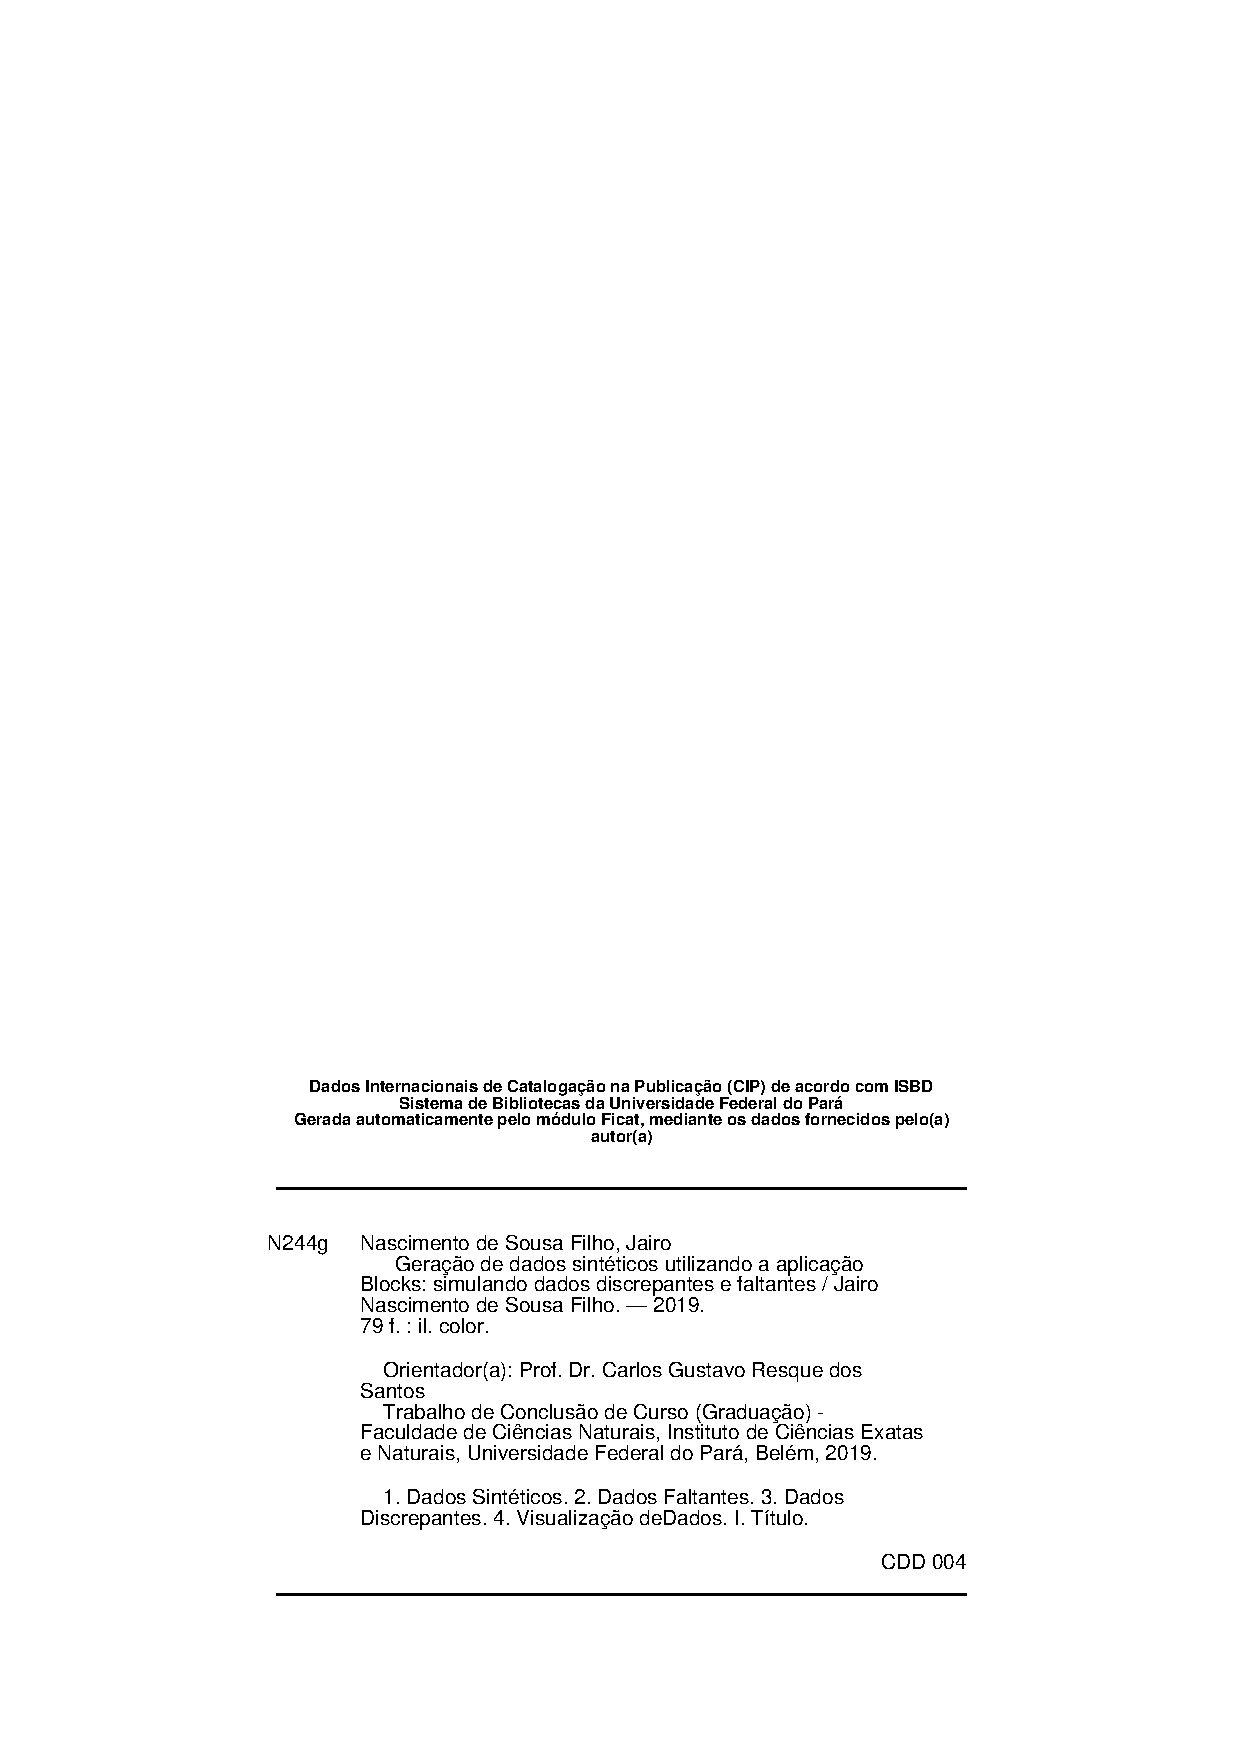
\includepdf{ficha.pdf}
\end{fichacatalografica}

% \begin{fichacatalografica}
% 	\sffamily
% 	\vspace*{\fill}					% Posição vertical
% 	\begin{center}					% Minipage Centralizado
% 	\fbox{\begin{minipage}[c][8cm]{13.5cm}		% Largura
% 	\small
	 
% 	\end{minipage}}
% 	\end{center}
% \end{fichacatalografica}
% ---

% ---
% Inserir errata
% ---
%\begin{errata}
%Elemento opcional da %\cite{NBR14724:2011}. Exemplo:

%\vspace{\onelineskip}

%FERRIGNO, C. R. A. \textbf{Tratamento de neoplasias ósseas apendiculares com
%reimplantação de enxerto ósseo autólogo autoclavado associado ao plasma
%rico em plaquetas}: estudo crítico na cirurgia de preservação de membro em
%cães. 2011. 128 f. Tese (Livre-Docência) - Faculdade de Medicina Veterinária e
%Zootecnia, Universidade de São Paulo, São Paulo, 2011.

%\begin{table}[htb]
%\center
%\footnotesize
%\begin{tabular}{|p{1.4cm}|p{1cm}|p{3cm}|p{3cm}|}
%  \hline
%   \textbf{Folha} & \textbf{Linha}  & \textbf{Onde se lê}  & \textbf{Leia-se}  \\
%    \hline
%    1 & 10 & auto-conclavo & autoconclavo\\
%   \hline
%\end{tabular}
%\end{table}

%\end{errata}
% ---

% ---
% Inserir folha de aprovação
% ---

% Isto é um exemplo de Folha de aprovação, elemento obrigatório da NBR
% 14724/2011 (seção 4.2.1.3). Você pode utilizar este modelo até a aprovação
% do trabalho. Após isso, substitua todo o conteúdo deste arquivo por uma
% imagem da página assinada pela banca com o comando abaixo:
%
% \begin{folhadeaprovacao}
% \includepdf{folhadeaprovacao_final.pdf}
% \end{folhadeaprovacao}
%
\begin{folhadeaprovacao}

  \begin{center}
    {\ABNTEXchapterfont\large\imprimirautor}

    \vspace*{\fill}\vspace*{\fill}
    \begin{center}
      \ABNTEXchapterfont\bfseries\Large\imprimirtitulo
    \end{center}
    \vspace*{\fill}
    
    \hspace{.45\textwidth}
    \begin{minipage}{.5\textwidth}
        \imprimirpreambulo
    \end{minipage}%
    \vspace*{\fill}
   \end{center}
        
   Conceito: \rule{3cm}{.1pt}
   
   \imprimirlocal, 1 de janeiro de 2019.
   
   \vspace{1cm}
   \begin{center}
   BANCA EXAMINADORA
   \end{center}
    

   \assinatura{\textbf{\imprimirorientador} - Orientador \\ UFPA}
   %\assinatura{\textbf{\imprimircoorientador} - Coorientador \\ UFPA}
   \assinatura{\textbf{Prof. Dr. Bianchi Serique Meiguins} - Membro Interno \\ UFPA}
   \assinatura{\textbf{MSc. Diego Hortêncio dos Santos}  - Membro Externo\\ UFPA}
   %\assinatura{\textbf{Nome Convidado 3} \\ SIGLA INSTITUIÇÃO}
      

  
\end{folhadeaprovacao}
% ---

% ---
% Dedicatória
% ---
\begin{dedicatoria}
  \vspace*{\fill}
  \centering
  \noindent
  \textit{Às pessoas extraordinárias que me assistiram nos melhores e piores momentos e me proporcionaram chegar aqui.} \vspace*{\fill}
\end{dedicatoria}
% ---

% ---
% Agradecimentos
% ---
\begin{agradecimentos}
Agradeço a Deus por permitir a oportunidade de desenvolver meu trabalho. Também agradeço a minha família por me dar suporte em todos os aspectos da minha vida. Também agradeço ao meu orientador e todos meus colegas do laboratório que me ajudaram incansavelmente a sanar minhas dúvidas. Aos meus amigos da faculdade estiveram comigo nos melhores e piores momentos, trabalhos e descontrações. Agradeço aos meus amigos fora da faculdade também que, por mais que estivessem distantes, também significam muito para mim.

\end{agradecimentos}
% ---

% ---
% Epígrafe
% ---
\begin{epigrafe}
    \vspace*{\fill}
	\begin{flushright}
		\textit{``Se o conhecimento pode criar problemas, não é através da ignorância que podemos solucioná-los.''\\
		(John F. Kennedy)}
	\end{flushright}
\end{epigrafe}
% ---

% ---
% RESUMOS
% ---

% resumo em português
\setlength{\absparsep}{18pt} % ajusta o espaçamento dos parágrafos do resumo
\begin{resumo}

	Este trabalho foi desenvolvido tendo como foco a aplicação de geração e visualização de dados sintéticos denominada Blocks,
	 a qual tem a função de produzir dados faltantes e discrepântes de forma sintética.
	A ferramenta em questão é composta por geradores chamados de Blocos, que por sua vez, podem ser utilizados de forma encadeada permitindo que sejam gerados comportamentos mais complexos.
	Os Blocos são utilizados de acordo com a categoria de geradores a serem utilizados, produzindo 
	 sequências de dados numéricas ou temporais; 
	 com distribuição probabilística aleatória;
	 funcionais, que utilizam outra dimensão como parâmetro;
	 acessórios, os quais adicionam formatação ou valor para os dados a partir de formas geométricas.
	Adicionalmente, o Blocks permite que os dados gerados sejam visualizados a partir de um gráfico do tipo Coordenadas Paralelas que é apresentado na tela inicial da aplicação.
	Como objetivos norteadores desse estudo são apontados a modelagem, visualização e avaliação da geração de dados sintéticos faltantes e discrepantes.
	Por fim, a validação desta pesquisa foi realizada com a utilização de técnicas de visualizações tendo como foco o comportamento das dimensões analisadas.

 \textbf{Palavras-chave}: Dados Sintéticos, Dados Faltantes, Dados Discrepantes, Visualização de Dados.
\end{resumo}

% resumo em inglês
\begin{resumo}[Abstract]
 \begin{otherlanguage*}{english}
	This work was developed focusing on the application of synthetic data generation and visualization called Blocks,
	which has the function of producing missing data and outliers synthetically.
	The tool is composed of generators called Blocks, that can be used in a chained way allowing more complex behaviors to be generated.
	Blocks are used according to the category of generators to be used, producing
	numeric or temporal data sequences;
	with random probability distribution;
	Function, using another dimension as a parameter;
	accessories, which add formatting, or value to the data from geometric shapes.
	Additionally, Blocks allows the generated data to be viewed from a Parallel Coordinates graph that is displayed on the application's home screen.
	The guiding objectives of this study are the modelling, visualization and evaluation of missing synthetic data and synthetic outliers generation.
	Finally, the validation of this research was performed using visualization techniques focusing on the behavior of the analyzed dimensions.

   \vspace{\onelineskip}
 
   \noindent 
   \textbf{Keywords}: Synthetic Data, Missing Data, Outliers, Data Visualization.
 \end{otherlanguage*}
\end{resumo}

% ---

% ---
% inserir lista de ilustrações
% ---
\pdfbookmark[0]{\listfigurename}{lof}
\listoffigures*
\cleardoublepage
% ---

% ---
% inserir lista de quadros
% ---
% \pdfbookmark[0]{\listofquadrosname}{loq}
% \listofquadros*
% \cleardoublepage
% ---

% ---
% inserir lista de tabelas
% ---
\pdfbookmark[0]{\listtablename}{lot}
\listoftables*
\cleardoublepage
% ---

% ---
% inserir lista de abreviaturas e siglas
% ---
\begin{siglas}
  \item[JSON] JavaScript Object Notation
  \item[CSV] Comma Separated Values
  \item[DSV] Delimiter Separated Values
  \item[TSV] Tabular Separated Values
  \item[TSG] Threat Streaming Generator
  \item[XML] Extensible Markup Language
  \item[SOAP] Simple Object Access Protocol
  \item[REST] Representational State Transfer
  \item[HTTP] HiperText Transfer Protocol
  \item[MCAR] Missing Completely At Random
  \item[MAR] Missing At Random
  \item[MNAR] Missing not At Random
  \item[SVM] Support Vector Machine
  \item[CARS] Context-Aware Recommender Systems
  \item[UC] Use Case
  \item[SMV] Selectable Mode Vocoder
  \item[WSDL] Web Services Description Language
  
\end{siglas}
% ---

% ---
% inserir lista de símbolos
% ---
% \begin{simbolos}
%   \item[$ \Gamma $] Letra grega Gama
%   \item[$ \Lambda $] Lambda
%   \item[$ \zeta $] Letra grega minúscula zeta
%   \item[$ \in $] Pertence
% \end{simbolos}
% ---

% ---
% inserir o sumario
% ---
\pdfbookmark[0]{\contentsname}{toc}
\tableofcontents*
\cleardoublepage
% ---



% ----------------------------------------------------------
% ELEMENTOS TEXTUAIS
% ----------------------------------------------------------
\textual

% ----------------------------------------------------------
% Introdução (exemplo de capítulo sem numeração, mas presente no Sumário)
% ----------------------------------------------------------
\chapter{Introdução}
% ----------------------------------------------------------
	%Mostrar o que são dados sintéticos de forma geral.
	%Mostrar o problema que é a utilização de dados reais.
	%Mostrar o uso de dados sintéticos e principais locais de uso.
	%Mostrar a necessidade de um gerador de dados sintéticos.
	%Mostrar que já existem geradores de dados sintéticos.
	%Mostrar o diferencial do sistema que procuramos fazer.
	%Mostrar o que são dados ausentes (missing data)
	%Mostrar o que são dados discrepantes
	%Apresentar os Objetivos do Trabalho em conjunto dos métodos.

	Dados sintéticos são dados gerados por uma máquina a partir de outros dados, geradores, fórmulas matemáticas, funções, entre outros.
	Esses dados, apesar de não possuirem um comportamento comparável aos da realidade, podem ser aplicados de variadas formas.
	Quer seja substituindo/simplificando dados reais, a exemplo de dados previsíveis que podem ser substituídos por fórmulas ou funções, ou adicionando novos dados a partir de uma instância fazendo algumas alterações. \cite{pensamentos-dados-sinteticos}
	\cite{pensamentos-dados-sinteticos}
	\par
	Um problema muito complicado aumenta a demanda por dados sintéticos: confidencialidade dos dados.
	Ninguém quer ter seus dados sendo usados de forma arbitrária por empresas, mas todos querem melhores serviços.
	Logo, para melhorar a situação dos dois lados, os dados sintéticos podem atingir um grau de realismo - dependendo da ferramenta e da habilidade do operador - sem ter grandes problemas de privacidade. \cite{pensamentos-dados-sinteticos}
	\par
	Também, outro problema é a escassez dos dados.
	Este cenário é encontrado principalmente em lançamento de novas tecnologias ou tratamento de exceções.
	Então, a partir da amostra existente, gera-se novas instâncias, determinando novos padrões, logo, novos casos de teste ou de uso.
	\par
	Os dados podem ser variados, como um número, uma categoria, uma marcação de tempo, uma imagem, um áudio ou um vídeo.
	Portanto, para geração de dados sintéticos são exigidos vários tipos de métodos.
	Entre os mais conhecidos podem ser citados fórmulas matemáticas, redes neurais, interpolação de frames, embaralhamentos, aleatoriedade etc.
	\par
	Alguns métdos de geração podem gerar dados sintéticos muito simples.
	Sendo assim, uma forma de dar realismo aos dados é permitir que algumas instâncias sejam faltantes.
	Por exemplo, alguém pode se esquecer ou recusar responder uma informação, pode haver uma falha no disco rígido, entre outros.
	Logo, dados faltantes são considerados comuns em bases de dados reais.
	\par
	Dados faltantes podem assumir diferentes formas dependendo do seu contexto de análise.
	Na literatura são encontradas 3 formas: \emph{Missing Completely At Random} (MCAR), \emph{Missing At Random} (MAR) e \emph{Missing Not At Random} (MNAR).
	Basicamente o MCAR determina que a falta do dado é completamente aleatória.
	No MAR ainda é aleatório, mas é possível predizer o valor faltante a partir de uma dimensão correlacionada.
	O MNAR indica que o dado está faltante e o seu motivo não está dito na base de dados, ou seja, pode haver influência de contexto externo.
	\par
	Outra característica de base de dados reais é a existência de dados discrepantes.
	Estes são definidos como dados que saem do padrão, quer seja no valor ou na formatação. \cite{Aggarwal2012}
	Como exemplo de dados discrepantes podem ser citados uma falha no sensor ou um evento atípico.
	\par
	Dados discrepantes podem assumir dois tipos: dados ruidosos e dados anômalos.
	Um dado ruidoso ou simplesmente ruído, possui um baixo grau de discrepância.
	Já o dado anômalo - ou anomalia - possui um alto grau de discrepância, podendo até atrapalhar o entendimento do fenômeno e a visualização dos dados.
	\par
	Pensando em tornar acessíveis os dados sintéticos foi desenvolvido o software de código aberto e gratuito chamado de Blocks.
	O Blocks oferece vários geradores de dados sintéticos de diferentes categorias.
	Também permite encadeá-los para que os dados tenham cada vez mais complexidade.
	É possível gerar sequências, dados randômicos, correlacionar dimensões e adicionar acessórios como ruídos e dados faltantes.
	\par
	Por conseguinte, o objetivo é apresentar o Blocks e como gerar dados faltantes e discrepantes nessa aplicação.
	Também serão apresentados os geradores de dados faltantes desenvolvidos no âmbito deste trabalho.
	Feito isso, o Blocks permite que os dados sejam visualizados, então é interessante que essa funcionalidade seja analisada.
	Em suma, este trabalho vai apresentar o funcionamento do Blocks modelando e visualizando dados faltantes e discrepantes.
	\section{Motivação e Justificativa}
		O Blocks está inserido no nicho de geração de dados sintéticos.
		Há várias aplicações disponíveis para essa função de geração de dados.
		Contudo, o preço pode ser um obstáculo, bem como algumas funcionalidades que podem faltar como um \emph{Web Service} ou geradores como para dados discrepantes ou faltantes.
		Outros diferenciais podem ser citados como a performance na obtenção de grande volume de dados ou acréscimo de dados sintéticos em bases reais.

	\section{Objetivos}
		O objetivo geral deste trabalho é implementar e validar geradores de dados sintéticos faltantes e discrepantes utilizando a aplicação Blocks.
		Também, a aplicação Blocks é demonstrada desde sua estrutura, a interface gráfica e o uso dos geradores implementados.			
		E os objetivos específicos são:
		\begin{itemize}
			\item Implementar geradores de dados faltantes no sistema Blocks.
			\item Implementar geradores de dados discrepantes no sistema Blocks.
			\item Validar geradores de dados faltantes e discrepantes através de visualizações.
			\item Contribuir para o desenvolvimento geral do sistema Blocks.
		\end{itemize}
	\section{Estrutura do Trabalho}
		Este trabalho está organizado em 6 capítulos, o qual o presente capítulo trouxe uma contextualização do estudo dos dados sintéticos, faltantes, discrepantes, e também os objetivos do trabalho.
		O segundo capítulo trata da fundamentação teórica do trabalho, a qual busca embasar os conceitos utilizados durante o trabalho, bem como mostrar outros trabalhos e aplicações relacionadas.
		\par
		O terceiro capítulo visa dar mais detalhes sobre a arquitetura de \emph{software} do Blocks, com a apresentação de diagramas de classe, de sequência e casos de uso.
		O quarto capítulo apresenta o sistema blocks em seu funcionamento, interface gráfica, modos de geração de dados entre outros aspectos.
		\par
		No quinto capítulo estão as visualizações a partir dos modelos de dados, que por sua vez, possuem os métodos implementados de dados faltantes e discrepântes.
		No sexto capítulo, estão o resumo do trabalho apresentado, algumas considerações sobre os resultados e trabalhos futuros para a continuação da pesquisa. 
		Por fim, há um apêndice para mostrar os atalhos de teclados disponíveis no Blocks até o desenvolvimento desse trabalho.
% ---

\chapter{Fundamentação Teórica}
	Neste capítulo é apresentada uma pesquisa sobre a literatura dos dados sintéticos, discrepantes, faltantes,
	 bem como de arquivos, e serviços como \emph{Web Service} e base de dados.
	% Por que estou fazendo isso?
	% Qual a necessidade de um gerador de dados sintéticos?
	% Já existem aplicações? Quais os seus prós e contras?
	% Onde são aplicados os dados sintéticos.
	% Qual o desempenho? Quais os resultados? Discussão.

	% Escrever um overview. Principais funcionalidades. Multiplataforma. Forma de pagamento.
	% Funcionalidades Detalhadas.
	% Se houver softwares relacionados, explicar um pouco mais sobre.
	% Mostrar a foto.

	\section{Dados Sintéticos}
		Dados sintéticos foi definido como "qualquer dado produzido o qual possa ser aplicado a uma dada situação que não foi obtido por mensuração direta." \cite{mcgraw-hilleducation2016}.
		Como exemplo, Rubin \cite{rubin1993statistical} a introduziu um conjunto de dados completamente sintético.
		Com o objetivo de tornar anônimo os domicílios que participaram do censo daquela época.
		A questão da confidencialidade sempre foi uma característica necessária para dados divulgados, principalmente para dados pessoais.
		Os dados sintéticos possuem a possibilidade de serem alterados mantendo a mesma ideia, logo, representa os dados reais originais.
		Essa característica que ajudou na popularização dos dados sintéticos.
		\par
		A necessidade de dados sintéticos podem ser de várias formas, 
		desde a escassez de dados reais ou indisponibilidade;
		para teste de dados não usuais;
		para evitar lidar com questões de privacidade dos dados;
		teste de aplicação sem precisar modificar dados da aplicação de produção;
		criar teste de estresse da aplicação com \emph{Big Data} antes de criar versão para produção;
		bem como não ter a necessidade de adicionar os dados de teste manualmente. \cite{top15DatagenTools2019}
		\par
		A aplicabilidade dos dados sintéticos é ilimitada e é bastante explorada por setores cujos dados são pessoais como o financeiro \cite{lopez2012money} e da saúde \cite{bergeat2014french}.	
		Também são muito bem aplicáveis para exaustivos testes de segurança, os quais são necessários vários casos de teste
		pesquisador/analista de teste tem controle suficiente das características (fórmulas matemáticas ou regras de geração) e pode usar em um sistema de detecção de fraudes, por exemplo \cite{barse2003synthesizing}.
		
	
	\section{Arquivo}
		Gerar os dados não é o suficiente, para isso, é necessário oferecer uma forma pronta de uso para o usuário.
		Para isso, pode ser utilizado os arquivos.
		Segundo Tanenbaum arquivos são unidades lógicas de informação criadas por processos e gerenciados por sistemas operacionais.
		Também é um mecanismo de abstração ao usuário para leitura e escrita em disco.
		Para que isso funcione, são adotados algumas convenções.
		A primeira são os sistemas de arquivos.
		Basicamente, um sistema operacional adota um sistema de arquivos para personalizar a questão da leitura e escrita.
		Também, um arquivo possui uma extensão (nome.extensão) cuja esta dá mais informações a respeito do conteúdo do arquivo \cite{tanenbaum1995sistemas}.
		\par
		Os arquivos são amplamente utilizados na computação, e por conta da larga escala de uso, foram criadas várias extensões de arquivos.
		Toda linguagem de programação possui seu arquivo como .java para Java, .js para JavaScript e .py para Python.
		\par
		Também existem os arquivos cujos dados são acessados por várias plataformas. O XML é muito utilizado na Web e pela linguagem Java, o JSON (\emph{Javascript Object Notation}, ou em português Notação de Objeto Javacript) tomou uma parcela da web com o uso, principalmente, de APIs, e o CSV ( \emph{Comma Separated Values}) é largamente utilizado em aplicações de ciência de dados, por exemplo.
        \par
		%JSON
		E quanto ao JSON, \cite{json-rfc-8259} \cite{json-jsonOrg} este lançado em 2002, é uma formatação leve para troca de dados. 
		O uso é facilitado tanto para seres humano quanto para máquina.
		O JSON é um formato de texto que é independente de linguagem, mas foi baseado na notação de objeto do Javascript (ECMA-262, 1999).
		\par
		Quanto aos tipos de dados suportados, o JSON \cite{json-rfc-8259} é uma sequência de tokens. 
		Os tipos de tokens aceitos é do tipo \textit{object}, \textit{array}, \textit{string}, \textit{number} e nomes literais como \textit{false}, \textit{true} e \textit{null}.
		\par
		%CSV
		Outra extensão de arquivo é o CSV \cite{csv-rfc-4180} (comma-separated values, ou em português Valores Separados por Vírgula) o qual é um arquivo do tipo de texto MIME (Internet Media) \cite{mime-rfc-2048} que utiliza a encodificação de caracteres US-ASCII \cite{csv-rfc-7111}.
		Ao longo dos anos, seu uso foi consolidado para exportar dados entre vários softwares de tabelas (Microsoft suíte para Apple Suíte, por exemplo).
		A padronização do CSV demorou a ocorrer e por isso, vários outros estilos surgiram, a exemplo, o uso do CSV com ponto-e-vírgula (;).
		Outros estilos foram criados a ponto de ser chamado de arquivo DSV \cite{dsv}.
		Por conseguinte, outro estilo que teve notoriedade na troca de dados entre bancos de dados ou tabelas de dados foi o TSV \cite{tsv-iana}.
		A ideia é similar ao CSV, porém é utilizado uma tabulação em vez de vírgula.
		
		%\subsection{Banco de Dados}
	\section{Web Service}
		Um \emph{Web Service} \cite{webService-W3C} é definido como um software criado para suportar interoperabilidade entre máquinas através da rede computadores.
		Na história do \emph{Web Service} surgiram o Protocolo SOAP (Simple Object Access Protocol) que utiliza o WSDL (Web Services Description Language) como uma interface descrita em um formato processável por máquinas \cite{webService-W3C} e o modelo de arquitetura REST (Representational State Transfer) proposto por Fielding \cite{fielding2000architectural} que não utiliza o WSDL.
		Atualmente é predominante o uso de REST que em vez de exportar serviços como o SOAP, exporta os dados em si e não necessita do WSDL. \cite{soapVSrest}
		O REST foi criado em conjunto ao HTTP 1.1 e a sua principal característica é a utilização simplificada dos verbos do protocolo HTTP (GET, POST, PUT, HEAD, OPTIONS e DELETE) \cite{WSRestvsSOAP}
		%TODO: colocar exemplos de web services

	\section{Dados Ausentes}
		% O que são dados faltantes
		O termo dados ausentes ou dados faltantes significa que está faltando dados suficientes para se formar uma informação e
		compreender o fenômeno de interesse ao observar o conjunto de dados. \cite{patrickmcknight2007}
		% Porque dados podem faltar
		Esses dados podem ser perdidos ou não coletados em todas as etapas de obtenção de dados em uma situação real
		como um participante desistindo ou não respondendo parte da pesquisa,
		o pesquisador perdendo seu dispositivo de anotação,
		má operação ao salvar em dispositivos eletrônicos etc. \cite{patrickmcknight2007}
		\par

		% O impacto dos dados ausentes
		O grande impacto dos dados ausentes encontra-se quando faltam dados a ponto da pesquisa se tornar tendenciosa, inconclusiva ou inconsistente \cite{patrickmcknight2007}.
		Um exemplo seria uma pesquisa de avaliação de motos.
		Características como modelo, ano, preço, número de vendas e média de notas seriam coletadas.
		Contudo, ao salvar a pesquisa no mesmo disco rígido, a parte referida a um dos integrantes foi corrompida e, portanto, há uma ausência de dados.
		\par
		% Mecanismos de dados ausentes
		Para compreender e lidar melhor com os dados ausentes foram definidos os mecanismos de dados ausentes.
		Esses mecanismos são conceituados como a probabilidade de uma resposta ser observada ou estar faltando.
		Existem 3 mecanismos conhecidos como 
		faltando de forma completamente aleatória - \emph{MCAR  (Missing completely at random)};
		faltando de forma aleatória - \emph{MAR (Missing At Random)};
		faltando de forma não aleatória - \emph{ MNAR (Missing Not At random)} \cite{molenberghs2014handbook}.

		\subsection{MCAR}
			Um dado faltante é classificado como MCAR quando a probabilidade da resposta está faltando não é relacionada com outros valores do conjunto de dados nem com os dados que deveriam ser coletados.
			Vale ressaltar que é muito difícil relacionar este mecanismos nos conjuntos de dados reais \cite{molenberghs2014handbook} \cite{little2016missing}.
			Na tabela \ref{table: exemplo DA MCAR} os dados ausentes MCAR não apresentam correlação com outras propriedades para justificar o dado faltante. Portanto, não há como prever qual o valor do dado faltante.
			\begin{table}[h]
				\centering
				\caption{Exemplo de dados ausentes MCAR}
				\vspace{0.5cm}
				\label{table: exemplo DA MCAR}
				\begin{tabular}{r|lll}
				
					ID & Estação do ano & Fruta & Receita \\ % Note a separação de col. e a quebra de linhas
					\hline                               % para uma linha horizontal
					1 & Verão     & Laranja & Alta  \\
					2 & Inverno   & Laranja & Baixa \\
					3 & Verão     & Morango & Baixa \\
					4 & Inverno   & Morango & Baixa \\
					5 & Outono    &         & Baixa       % não é preciso quebrar a última linha

				\end{tabular}
				\bigskip
				\\
				\footnotesize Fonte: O autor do trabalho.
			\end{table}
		
		\subsection{MAR}
			Quanto ao MAR, este é definido como a probabilidade da resposta está faltando depende dos dados obtidos, mas não está relacionado com dados fora da amostra coletada.
			Este é o mecanismo mais fácil de utilizar técnicas de imputação de dados, pois permite a predição de resultados. \cite{molenberghs2014handbook} \cite{little2016missing}
			Na tabela \ref{table: exemplo DA MAR e DA MNAR} é possível visualizar um exemplo de dados ausentes do mecanismo MAR.
			Neste caso, assume-se que há correlação entre os valores da tabela e por isso, por predição, assume-se que o valor faltante seja "Alta".
			\begin{table}[h]
				\centering
				\caption{Exemplo de dados ausentes MAR}
				\vspace{0.5cm}
				\label{table: exemplo DA MAR e DA MNAR}
				\begin{tabular}{r|lll}
				
					ID & Estação do ano & Fruta & Receita \\ % Note a separação de col. e a quebra de linhas
					\hline                               % para uma linha horizontal
					1 & Verão     & Laranja & Alta  \\
					2 & Primavera & Laranja & Alta  \\
					3 & Verão     & Limão   & Alta  \\
					4 & Inverno   & Limão   & Baixa \\
					5 & Verão     & Laranja &         % não é preciso quebrar a última linha
				
				\end{tabular}
				\bigskip
				\\
				\footnotesize Fonte: O autor do trabalho.
			\end{table}
		
		\subsection{MNAR}
			Quanto ao MNAR, este é definido como a probabilidade da resposta está relacionada com os dados que não estão presentes na amostra. \cite{molenberghs2014handbook} \cite{little2016missing}
			Isto é, por algum motivo que não está no conjunto de dados, há dados ausentes.
			Este mecanismo permite a geração de hipóteses para justificar a ausência desses dados. %Professor Bianchi adora fazer isso.
			Ainda na tabela \ref{table: exemplo DA MAR e DA MNAR} visualiza-se um exemplo de dados ausentes do mecanismo MNAR.
			O fato da receita de laranja não ter sido divulgada neste registro pode indicar que o produtor não queira preocupar os possíveis investidores (ou partes interessadas no agronegócio) devido uma possível baixa nos rendimentos.
			
	\section{Dados Discrepantes}
		%O que são dados discrepantes
		Dados discrepantes ou \emph{outliers} são dados que são significativamente diferentes dos outros dados do conjunto de dados.
		%Por que são causados
		Também conhecidos como anomalias ou dados desviantes esses dados podem ser gerados, em geral, quando o sistema se comporta de forma não usual.
		Por isso, a presença e a frequência de dados discrepantes também são informações relevantes para com o conjunto de dados.
		Exemplos desta relevância são para sistemas de detecção de invasão, fraudes de cartão de crédito, diagnósticos médicos e estudos geológicos \cite{Aggarwal2012}.
		%Como identificá-los
		\par
		Para identificar os dados discrepantes é um pouco mais subjetivo, isto é, mais dependente de critérios feitos por quem está avaliando, assim como de qual aplicação está sendo extraído o conjunto de dados.
		Contudo, existe um espectro de dados normais para discrepantes como pode ser visto na figura \ref{fig:Aggarwal}.
		Nesta figura, justamente o limiar entre os normais para os ruídos e anomalias não são precisamente definidos,
		mas algoritmos de detecção de discrepância podem dar pontuação de discrepância para cada dado e utilizar este nível \cite{Aggarwal2012}.

		%figura
		\begin{figure}[!h]
			\centering
			\caption{Exemplo de escala de discrepância}
			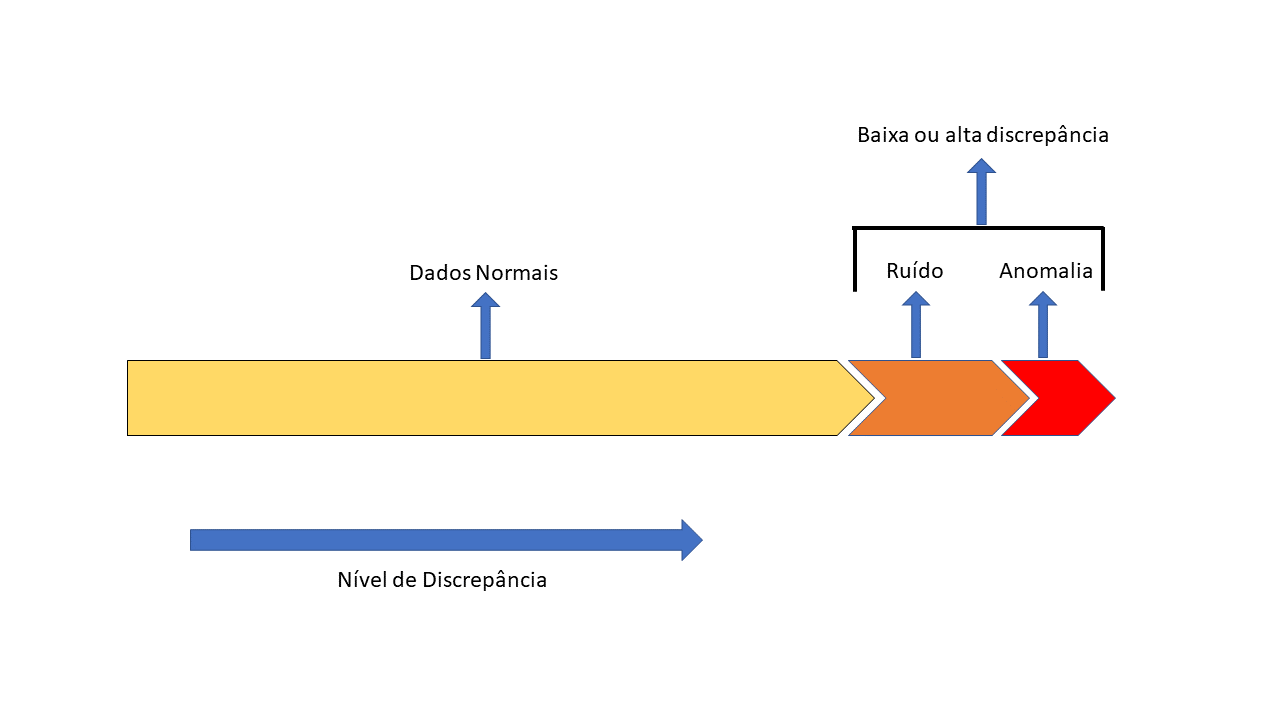
\includegraphics[width=\linewidth]{./figures/FundamentacaoTeorica/ExemploDeDiscrepancia.png}
			\label{fig:Aggarwal}
			\footnotesize Fonte: Adaptado de \cite{Aggarwal2012}.
		\end{figure}
		

		%Como lidar com eles
		E se o dados discrepantes não forem tratados, eles podem gerar problemas como 
		redução da precisão do modelo de dados,
		aumentar a complexidade do modelo e
		dificultar e legibilidade dos dados \cite{Aggarwal2012} \cite{rathi_2019}.
		E para tratá-los, as formas convencionais são 
		remoção de instâncias,
		filtro de dimensões,
		combinar essas formas convencionais com algoritmos de validação (como o k-fold);
		ou detecção de anomalias (como baseado em clusterização, \emph{Selectable Mode Vocoder} (SMV) ou densidade.
	
		\subsection{Dados Ruidosos e Anômalos}
			%O que são dados ruidosos
			Dados ruidosos são dados indesejaveis, dimensões ou instâncias que não estão relacionadas com o fenômeno estudado.
			Em geral, dados ruidosos fazem com que algoritmos de aprendizado de máquina encontrem padrões incoerentes \cite{rathi_2019}.
			Dados ruidosos e dados anômalos (ver figura \ref{fig:ruidoAnomalo}) diferenciam-se, basicamente, na sua facilidade de percepção em uma visualização e no seu grau de impacto ao inferir sobre os dados.
			\begin{figure}[h!]
				\centering
				\caption{
					Exemplo de ruído e de anomalia. 
					O item A é um exemplo de dado ruidoso, pois desvia-se levemente do padrão dos dados - uma reta.
					Quanto ao Item B este descaracteriza significativamente o padrão dos dados - este é um exemplo de dado anômalo.
				}
				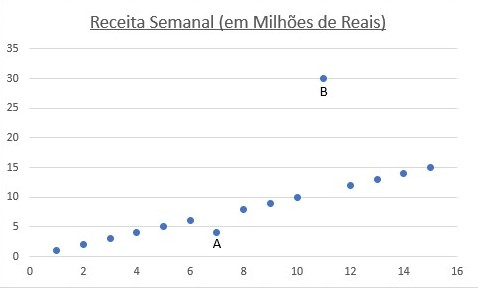
\includegraphics[width=\linewidth]{./figures/FundamentacaoTeorica/ExemploRuidoAnomalo.jpg}
				\label{fig:ruidoAnomalo}
				\footnotesize Fonte: O autor do trabalho.
			\end{figure}
			\par
			
			%Quais os tipos
			Segundo Rathi (2019), dados discrepantes quando em formato tabular podem ser classificados de três formas:
			\begin{itemize}
				\item anormalidades;
				\item dimensões irrelevantes;
				\item instâncias ruídas.
			\end{itemize}
			As anormalidades são irregularidades tanto nas dimensões dos dados ou no evento estudado.
			As características irrevelentes são aquelas que não ajudam a explicar o fenômeno.
			E as instâncias ruídas são aquelas que desviam a forma dos outros dados. \cite{rathi_2019}
			\par
			Na figura \ref{fig:Rathi} podem ser observados exemplos das classificações definidas por Rathi (2019) para dados discrepantes quando apresentados em formato tabular.

			\begin{figure}[h!]
				\centering
				\caption{Exemplo de anormalidades; dimensões irrelevantes e instâncias ruídas.}
				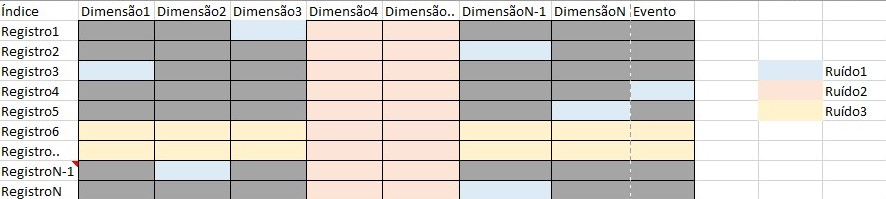
\includegraphics[width=\linewidth]{./figures/FundamentacaoTeorica/ExemploClassificacaoRuido.jpg}
				\label{fig:Rathi}
				\footnotesize Fonte: Adaptado de \cite{rathi_2019}.
			\end{figure}
			
% \chapter{Trabalhos Relacionados}
% 	Nesse capítulo serão apresentados trabalhos acadêmicos e aplicações as quais possuem correlação com este estudo.
% 	Para isso, foram feitas análises sobre os trabalhos para identifcar semelhanças e diferenças pontuais.
% 	Essa análise foi feita com o fim de comparar os trabalhos e identificar contribuições, suprir necessidades e captar trabalhos futuros.

	\section{Trabalhos Acadêmicos Relacionados}
		\cite{albuquerque2011synthetic} descreveu um \emph{framework} capaz de gerar dados sintéticos multidimensionais.
		O sistema como mostra a figura \ref{fig:albuquerque} recebe um \emph{input} que representa algumas propriedades do conjunto de dados como número de dimensões,
			uma distribuição de dados padrão,
			tipo de dado de cada dimensão entre outros.
		A partir disso, é criada uma função densidade de probabilidade, com o fim de gerar um conjunto de dados padrão.
		Essas funções podem ser ajustadas e modeladas através de objetos.
		Também, essas funções podem ser de 1, 2 ou 3 dimensões.
		Adicionalmente, pode-se haver ruídos, para simular as irregularidades encontradas em conjunto de dados reais.
		\par
		O framework apresentado também possui uma interface gráfica para auxiliar o usuário a configurar o conjunto de dados, bem como gerá-lo. 
		Contudo, não foi encontrado uma interface para pré-visualização dos futuros dados gerados.
		Quanto aos tipos de dados, estes são restritos aos numéricos, quer sejam inteiros ou de ponto flutuante.
		No texto, nada foi citado sobre dados faltantes ou discrepantes.    
		\begin{figure}[h!]
			\centering
			\caption{Visão Geral de geração de dados.}
			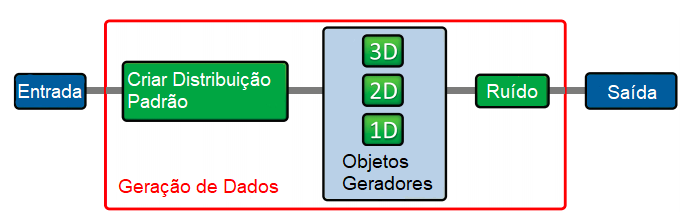
\includegraphics[width=\linewidth]{./figures/TrabalhosRelacionados/Albuquerque10.png}
			\label{fig:albuquerque}
			\footnotesize Fonte: Adaptado de \cite{albuquerque2011synthetic}.
		\end{figure}

		\cite{wang2013sketchpadn} apresentou uma aplicação chamada SketchPad cujo principal diferencial é a capacidade de modelar, através de desenho, o comportamento das dimensões do conjunto de dados sintéticos. A priori, o usuário pode iniciar o processo de geração através do zero, de um conjunto de dados já existente, ou um conjunto de dados aleatório. A partir disso, o usuário visualiza os dados no gráfico - que pode ser as coordenadas paralelas ou o \emph{scatterplot} - e pode modificá-lo através de cliques e arrastos. Por conseguinte, os dados podem ser gerados e isto também serve como retroalimentação do sistema. Na figura \ref{fig:sketchpad} é possível visualizar a visão geral do funcionamento do SketchPad como a introdução de dados, visualização e modelação utilizando o gráfico Coordenadas Paralelas e o espaço para desenho chamado de \emph{Touchpad n-d} e a criação ou modificação de um conjunto de dados.
		\begin{figure}[h!]
			\centering
			\caption{Visão Geral de geração de dados do Sketchpad.}
			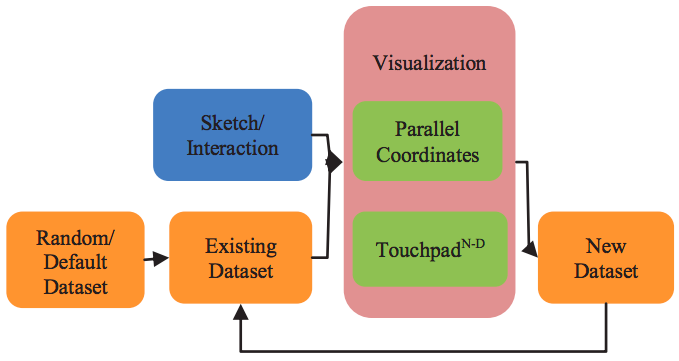
\includegraphics[width=\linewidth]{./figures/TrabalhosRelacionados/Wang11.png}
			\label{fig:sketchpad}
			\footnotesize Fonte: Adaptado de \cite{wang2013sketchpadn}.
		\end{figure}

		\cite{liu2016synthetic} criou um gerador de dados sintéticos a partir de avaliação de regras de aprendizagem. O sistema funciona criando regras de aprendizagem - usando algoritmos de árvore de decisão como o ID3 - baseado em dados de entrada construindo correlações entre os dados. Na figura \ref{fig:liu} é possível visualizar uma árvore de decisão. Durante a leitura do conjunto de dados de entrada é feita a árvore de decisão e, concomitantemente, são geradas as regras de aprendizagem. Essas regras são utilizadas para gerar amostras de dados sintéticos. As regras são interessantes tanto para reutilizar os dados quanto para facilitar em determinar o comportamento dos dados.
		\begin{figure}[h!]
			\centering
			\caption{Exemplo de árvore de decisão para jogar tennis criado a partir de regras encontradas em um conjunto de dados.}
			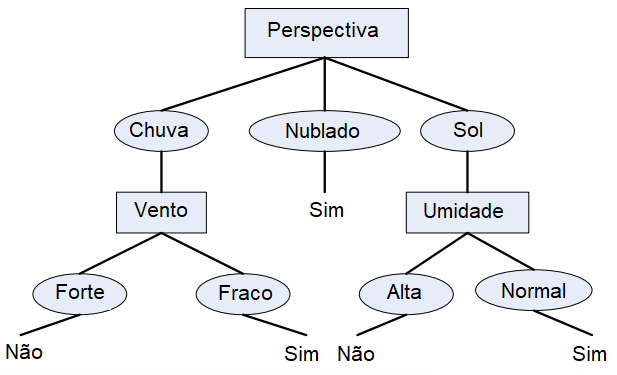
\includegraphics[width=\linewidth]{./figures/TrabalhosRelacionados/Liu13.png}
			\label{fig:liu}
			\footnotesize Fonte: Adaptado de \cite{liu2016synthetic}.
		\end{figure}

		\cite{garcia2011prototype} criaram um sistema de geração de dados sintéticos pensado para desenvolvedores que buscam testar de forma eficiente e exaustiva a sua aplicação. Esses dados pode ser configurados (ver figura \ref{fig:garcia}) de acordo com as preferências do usuário. As dimensões de dados seguem alguns padrões como a partir de fontes externas (Arquivos, Bibliotecas, Base de dados) Sequencial, Constante, Funcional, Intervalo ou Lista de valores. Contudo, os geradores, para alterar o comportamento dos dados, depende apenas dos parâmetros e não é possível misturar os geradores.
		\begin{figure}[h!]
			\centering
			\caption{Exemplo da interface do usuário para configuração do gerador de dados.}
			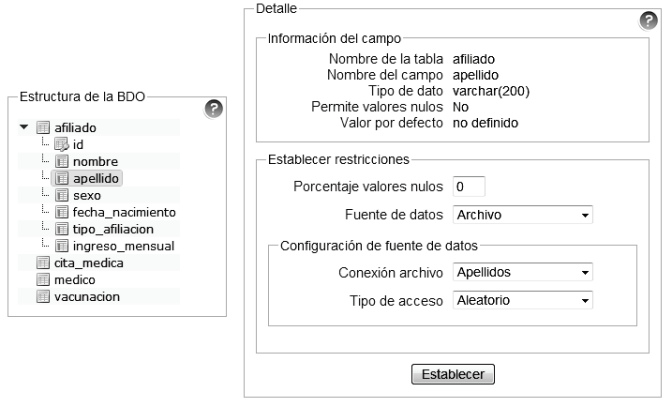
\includegraphics[width=\linewidth]{./figures/TrabalhosRelacionados/Garcia18.png}
			\label{fig:garcia}
			\footnotesize Fonte: \cite{garcia2011prototype}.
		\end{figure}

		\cite{kofinas2018methodology} criou uma metedologia para gerar dados sintéticos para simular consumo de água.
		A metodologia é avaliada por meio de algoritmos de validação - como a visualização dos resultados e fórmulas.
		\par
		Como pode ser visto na figura \ref{fig:kofinas}, a geração dos dados é feita a partir de 2 fases.
		A fase 1 investiga a distribuição dos dados.
		Esta fase, primeiramente transforma dados numéricos em séries temporais de 30 segundos.
		Em alguns casos, não há registro, para isso, é criada uma tabela de incidentes e posteriormente uma probabilidade de existência de registro para que sejam encontradas as classes usadas para construção do histograma de Pearson \cite{dean2009descriptive}. 
		Por fim, são comparadas funções de distribuição com a atual com o objetivo de encontrar a que mais se aproxima.
		\par
		A fase 2 trata da geração de dados sintéticos utilizando a distribuição criada na fase 1 para gerar os dados para vinte e quatro horas, respeitando as características diferenciadas para dias de semana e finais de semana.
		Apesar de o trabalho ter como principal foco a calibração, modelagem e geração dos dados, não foi disponibilizada uma interface gráfica ao usuário para utilização das visualizações e geração dos dados faltantes e discrepantes.
		\par
		
		\begin{figure}[h!]
			\centering
			\caption{Fluxo de passos para geração dos dados sintéticos.}
			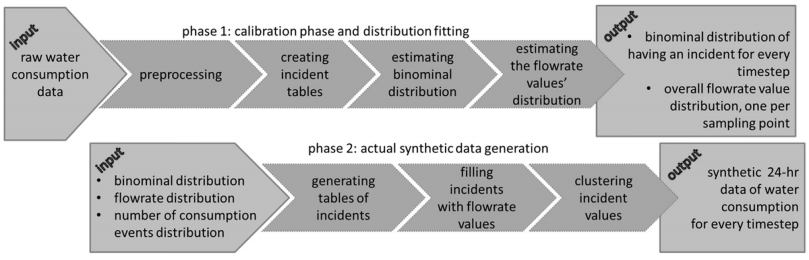
\includegraphics[width=\linewidth]{./figures/TrabalhosRelacionados/Kofinas21.png}
			\label{fig:kofinas}
			\footnotesize Fonte: Adaptado de \cite{kofinas2018methodology}.
		\end{figure}

		No estudo realizado por \cite{sakshaug2014nonparametric} foi aplicado um procedimento de simulação não paramétrica para geração de dados sintéticos de variáveis contínuas com o foco em pequenas áreas geográfica.
		A diferença entre a geração paramétrica e a não paramétrica é que a primeira utiliza valores sintéticos de uma distribuição normal e o não paramétrico não é baseado em distribuição. 
		Segundo a avaliação do autor os dados sintéticos tiveram validade moderadamente alta em seus testes, mas ressalta a limitação do método não paramétrico. 
		Em geral, o método não paramétrico se mostrou promissor para geração de dados sintéticos para pequenas áreas geográficas, mas faltam testes mais aprofundados como dados de pesquisa em larga escala para substituir os dados reais por dados sintéticos em centros de dados de pesquisa.
		Na figura \ref{fig:SakshaugandRaghunathan} é possível observar a comparação dos resultados da média da simulação paramétrica e da não paramétrica para cada atributo.
		Na simulação não paramétrica as médias dos dados sintéticos e reais ficam bem próximas, com exceção da Idade, apresentando um bom resultado para a troca de dados reais para dados sintéticos.
		\begin{figure}[h!]
			\centering
			\caption{Comparação da média dos dados reais e sintéticos na simulação paramétrica e não paramétrica.}
			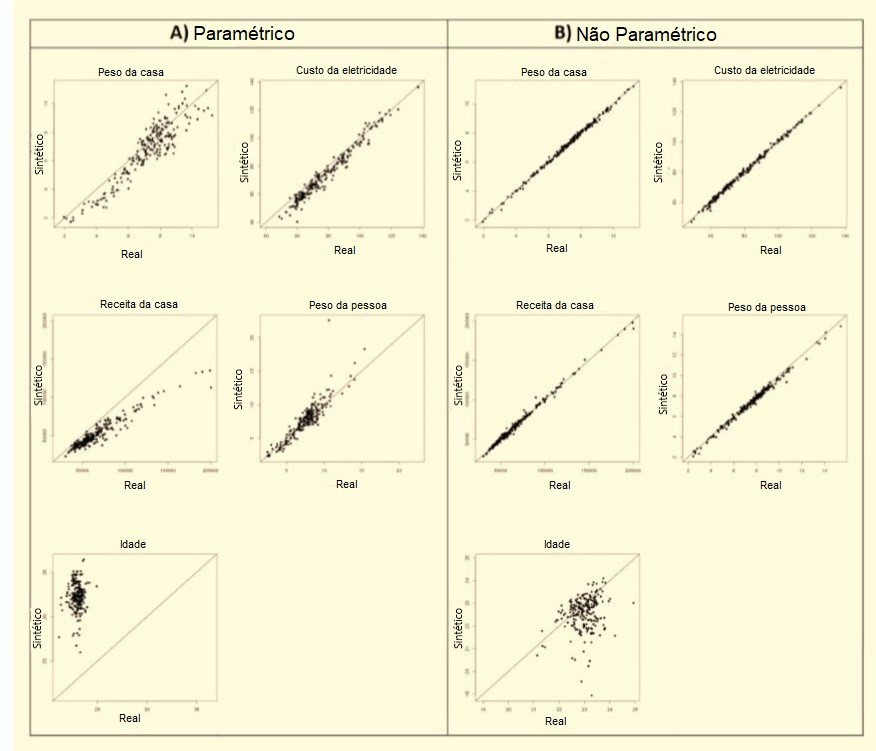
\includegraphics[width=\linewidth]{./figures/TrabalhosRelacionados/SakshaugandRaghunathan.jpg}
			\label{fig:SakshaugandRaghunathan}
			\footnotesize Fonte: Adaptado de \cite{sakshaug2014nonparametric}.
		\end{figure}

		O projeto \emph{Threat Streaming Generator} (TSG) visa criar um gerador de dados sintéticos realistas com foco em dados para testes.
		É mostrado o fluxograma dos processos do TSG na figura \ref{fig:whitingetal}.
		Primeiramente são definidos qual o tipo de conjunto de dados vai ser gerado.
		Em seguida são dadas três possilidades ao usuário de inserir o ambiente e a ameaça: manualmente, através da ferramenta TSG e outras fontes.
		Por fim, esses dados são analisados por especialistas os quais são responsáveis pela qualidade do conjunto de dados gerado.
		O projeto é bem competente para desenvolvimento de dados sintéticos, inclusive com a validação pelos especialistas, o qual pode elevar o custo financeiro para geração dos dados. \cite{whiting2008creating}
		\par
		\begin{figure}[h!]
			\centering
			\caption{Fluxo de passos para geração dos dados sintéticos.}
			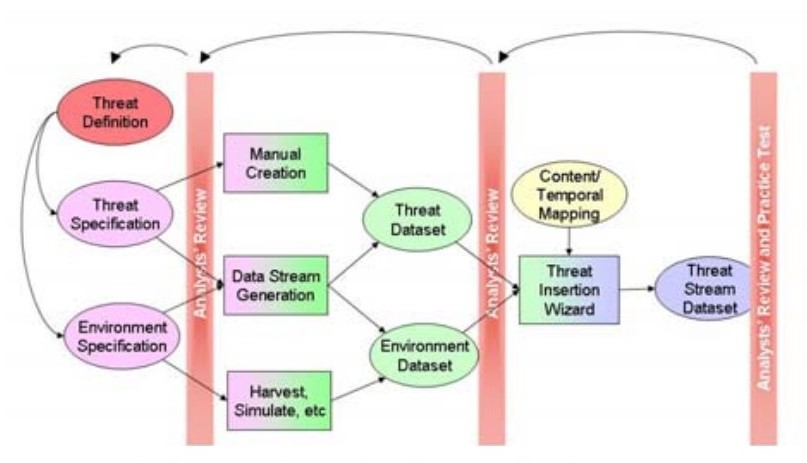
\includegraphics[width=\linewidth]{./figures/TrabalhosRelacionados/whitingetal.jpg}
			\label{fig:whitingetal}
			\footnotesize Fonte: Adaptado de \cite{whiting2008creating}.
		\end{figure}

		Com o foco em CARS (Context-Aware Recommender Systems - Sistemas de Recomendação sensíveis ao contexto), o DataGenCARS \cite{delCarmenRodrguezHernndez2017} é uma ferramenta para gerar dados sintéticos de forma flexível e prática.
		Permitindo que o usuário possa inserir os tipos de perfis do usuário, tipos de contexto e itens, misturar dados sintéticos e dados reais com o objetivo de aumentar o realismo dos dados gerados.
		\par
		Na figura \ref{fig:DataGenCARS} mostra-se o funcionamento do DataGenCARS.
		De início a ferramenta mostra que é possível, de forma opcional, expandir outros conjuntos de dados bem como analisá-los estatisticamente.
		Mesmo assim, devem ser definidos os esquemas de contexto de usuários, itens e configuração da geração para que se tenha o conjunto de dados.
		Dentro do tema que foi especificado (CARS) o DataGenCARS permite gerar dados de forma satisfatória bem como validar por meio de visualizações, mas não foi citado um tratamento para geração de dados faltantes e discrepantes.
		\par
		\begin{figure}[h!]
			\centering
			\caption{Fluxo de passos para geração dos dados sintéticos.}
			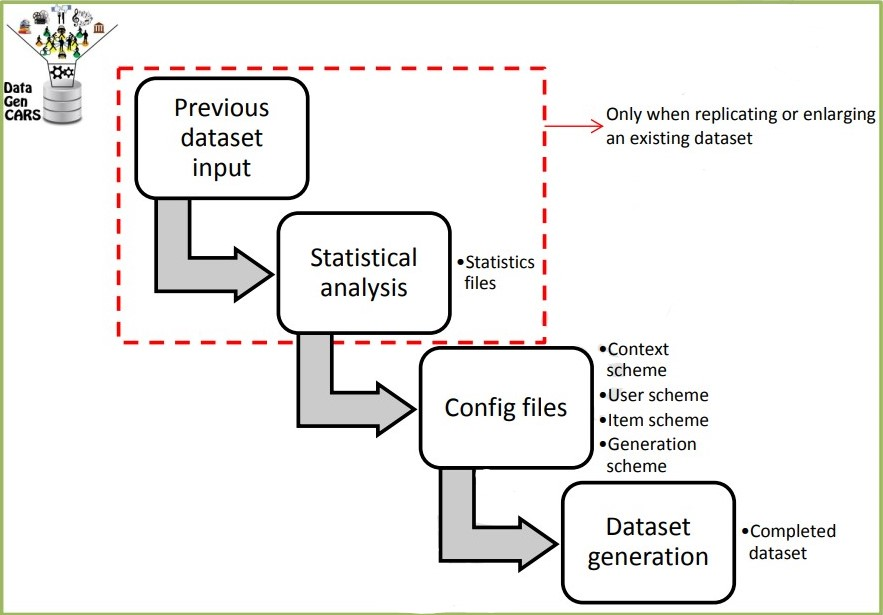
\includegraphics[width=\linewidth]{./figures/TrabalhosRelacionados/DataGenCARS.jpg}
			\label{fig:DataGenCARS}
			\footnotesize Fonte: Adaptado de \cite{delCarmenRodrguezHernndez2017}.
		\end{figure}

		Pensando em oferecer confidencialidade aos dados governamentais, \cite{Larsen2012} desenvolveram um gerador de dados sintéticos que alia regressão de quartis com imputação de dados em dados faltantes a partir de dimensões similares (imputação \emph{hot deck} \cite{andridge2010review}) e troca de classificação.
		A predição de regressão de quantis é feita para proteger dados sensíveis a partir de dados não sensíveis,
		 isto é, o conjunto de dados finais são compostos por dimensões reais - os não sensíveis - e sintéticos - para dimensões sensíveis.
		Em alguns casos os dados sintéticos são similares aos reais e para isso foi utilizado a imputação \emph{hot deck} junto com a troca de classificação, para garantir a aleatoriedade e confidencialidade dos dados.
		Contudo, nada foi citado sobre a geração de dados sintéticos ou faltantes.
        \par
        Dos trabalhos realizados, nem todos apresentaram uma interface gráfica ao usuário, ou variedade de geradores, com tratamento de dados faltantes ou discrepantes. Também sobre a validação por visualização poucos trabalhos apresentam integração dos dados gerados com uma ferramenta de visualização em tempo real.
		%Artigo sem figura.

	\section{Aplicações Relacionadas}

		DTM Data Generator \cite{DTMDataGenerator} é uma plataforma de geração de dados sintéticos que existe desde 1998.
		Esta possui suporte para geração de dados em arquivos, em banco de dados, também para \emph{Big Data}.
		Possui suporte multiplataforma, através da versão \emph{multiplatform runtime}, contudo esta é limitada quando comparado à versão Windows, o qual suporta a versão para servidor também.
		É válido destacar que o DTM Data Generator é um software pago para utilização oferecendo uma versão para testes.
		Além disso, há categorias de versões pagas, que vão desde limitações de geração (Standart - Professional) à vantagens mais técnicas (Professional - Enterprise).
		\\
		\par
		O DTM Data Generator possui uma vasta coleção de funcionalidades, as quais são acrescentadas de acordo com a versão do software.
		Adotando a versão mais cara, a lista de funcionalidades é composta por geração de dados em JSON, XML, CSV ou geração por separador customizado.
		Também permite gerar dados por arquivo DSN (Database Source Name), gerar dados por linha de comando e gerar um arquivo SQL para que não seja necessário conexão com banco de dados.
		\par
		É possível gerar cerca de nove vírgula dois sextilhões de registros por geração, modos de atualizar dados existentes (adicionar, substituir e ofuscar dados pessoais), e suporte para bibliotecas de dados realistas.
		A plataforma disponibiliza entrada de dados através de SQL, XML, JSON, pela WEB através de HTTP ou FTP, XLSM, arquivos de texto e \emph{scripts} em Python.
		Também é possível visualizar e testar os dados gerados, bem como gerá-los nos principais arquivos de texto (TSV, CSV, DSV, JSON, XML) e banco de dados (MS SQL Server, Oracle, DB2, MySQL, PostgreSQL, Informix, Sybase, SQLite e Firebird). 
		\par
		Há uma suíte de produtos relacionados fornecidos pela DTM soft. 
		Além do gerador de dados, 
			há o gerador de dados XML para teste de aplicação (\emph{DTM Test XML Generator});
			um gerador de planilhas Excel (\emph{DTM Data Generator for Excel});
			testador exaustivo - teste de estresse - de banco de dados (\emph{DTM DB Stress});
			Bem como editor, visualizador (\emph{DTM Data Editor}), comparador e sincronizador de banco de dados (\emph{DTM Data Comparer}), entre outros.
		Não foi encontrado uma documentação com mais detalhes dos geradores e se há suporte para geração de dados faltantes, bem como discrepantes.

		\begin{figure}[h!]
			\centering
			\caption{Usando o DTM Data Generator.}
			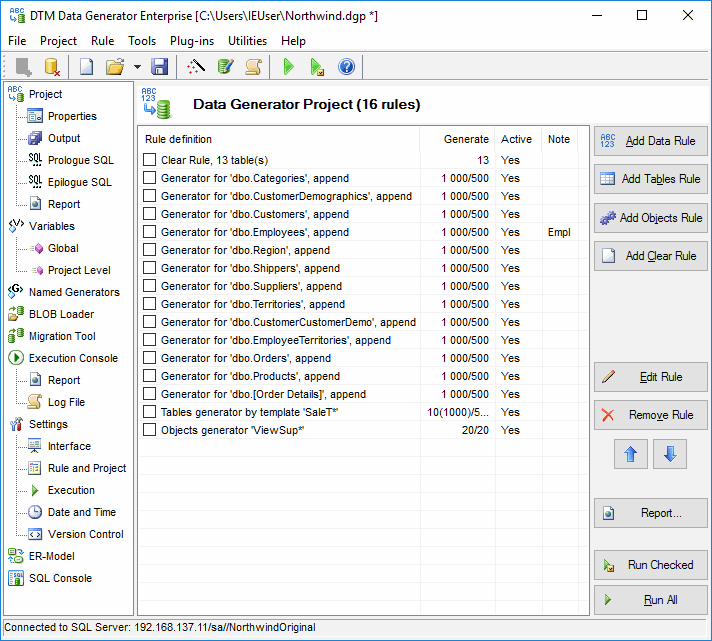
\includegraphics[width=\linewidth]{./figures/TrabalhosRelacionados/DTMDataGenerator.png}
			\label{fig:DTMDG}
			\footnotesize Fonte: \cite{DTMDataGenerator}.
		\end{figure}

		O SQL Data Generator \cite{RedgateSQLDataGenerator} é um software que compõe uma suíte de ferramentas (chamada de SQL Toolbelt) da Red Gate.
		O software é exclusivo para o ecossistema Windows, com suporte ao Windows 7 ou superior, à versão Windows Server, SQL Server (2008 ao 2017), .NET e Oracle.
		Este produto é distribuido através de licenças pagas e vitalícias, com atualizações gratuitas e no mínimo 1 ano de suporte gratuito.
		Vale ressaltar que é possível testar o produto por 14 dias gratuitamente.
		\par
		O \emph{SQL Toolbelt} tem funcionalidades bem delimitadas e a função do \emph{Data Generator} é popular um banco de dados. 
		A população da base de dados é feita ao escolher, primeiramente, uma tabela do banco.
		A partir disso, escolhe-se um gerador para cada coluna da tabela.
		Um gerador tem classificação fortemente baseada na realidade, isto é, possui geradores como palavras relacionadas à compras, pagamentos, pessoas (primeiro e último nome), dado geográficos e afins.
		\par
		A ferramenta também disponibiliza a geração a partir de expressões regulares \emph{Regex generator} e \emph{scripts} em Python.
		Por se tratar de banco de dados, também há checagem e tratamento de \emph{constraints}, \emph{Foreign keys} e \emph{Dependencies}.
		\emph{O SQL Data Generator} também permite lidar com arquivos XML, quer seja para geração de valores XML, como utilizar como dados de entrada, além de mesclá-los com o \emph{Regex generator}.
		\par
		Quanto ao \emph{SQL Toolbelt} oferecido pela \emph{Red Gate}, ele conta com 2 versões, o completo com quartoze programas e o \emph{essentials} com dez.
		Entre os mais relevantes, pode-se citar o \emph{SQL Data Compare}, \emph{SQL Data Generator}, \emph{SQL Test}, \emph{SQL Backup Pro} e \emph{SQL Scripts Manager}.
		\par
		Na documentação do SQL \cite{RedgateSQLDataGeneratorDoc} é possível encontrar os geradores de dados sintéticos.
		Entre os exemplos estão gerador por \emph{regex}, importação de arquivo, lista ponderada etc.
		Não houve uma citação por um gerador de dados discrepantes ou faltantes,
		 contudo é possível criar geradores de dados manualmente utilizando XML em conjunto com classes pré-definidas.
		Também o uso de embaralhador de texto, bem como a lista ponderada seja possível gerar dados faltantes e discrepantes.
		\begin{figure}[h]
			\centering
			\caption{Usando o Redgate SQL Data Generator.}
			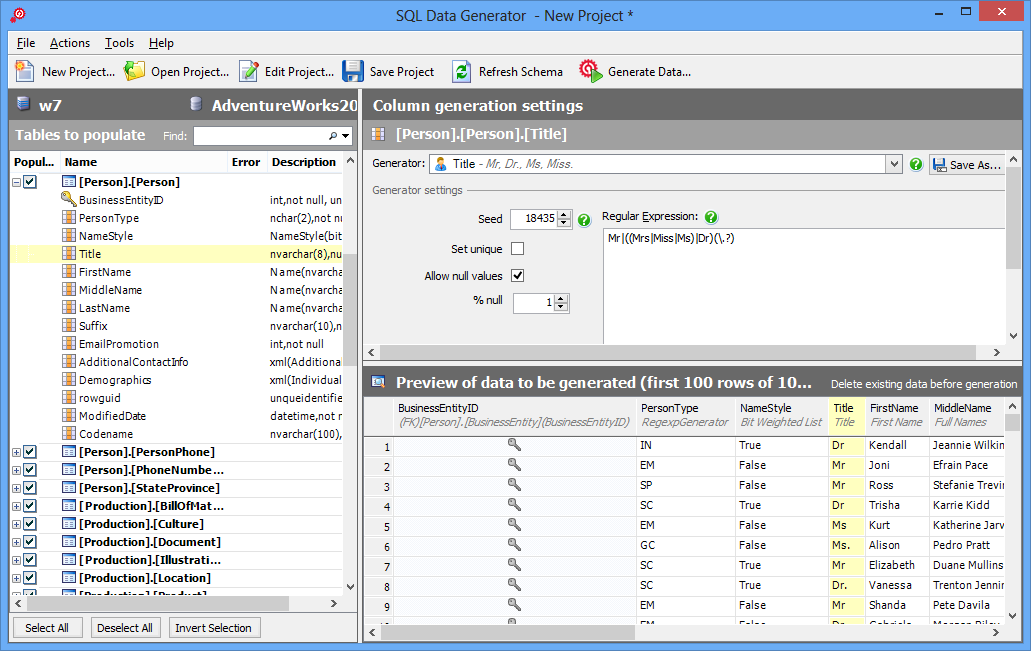
\includegraphics[width=\linewidth]{./figures/TrabalhosRelacionados/sql-data-generator.png}
			\label{fig:RedgateSQLDG}
			\footnotesize Fonte: \cite{RedgateSQLDataGeneratorDoc}.
		\end{figure}

		\emph{Microsoft Visual Studio} \cite{VSDataGenerator} é um pacote multiplataforma de programas da Microsoft para desenvolvimento de \emph{software}. 
		Este é composto por quatro versões (\emph{Express}, \emph{Professional}, \emph{Premium} e \emph{Ultimate}) e a opção de gerar dados para teste está disponível a partir da versão \emph{Premium}.
		O foco é permitir que verique o comportamento do banco de dados, sem relacioná-los com os dados da aplicação em produção.
		\par
		Para gerar os dados de teste, deve-se utilizar os geradores de dados (\emph{Data Generators}) que são correlacionados às tabelas do banco de dados.
			Os geradores podem ser dos mais primitivos (Binários, Inteiros, Data, \emph{Float}), como de Imagem, Dinheiro, Expressão Regular, Categórico, entre outros.
		Entre os geradores genéricos pré-definidos, não foi encontrado suporte para dados faltantes ou dados discrepantes, mas há a possibilidade de criar geradores personalizados.
		Também é disponibilizado um Plano de Geração de Dados (\emph{Data Generation Plan}), feito em XML, que contém informações do banco de dados, o tipo de dados de cada gerador e a quantidade de dados para ser gerado. 
		Este plano serve basicamente para reutilização da lógica de teste.
		\begin{figure}[h]
			\centering
			\caption{Usando o Microsoft Visual Studio.}
			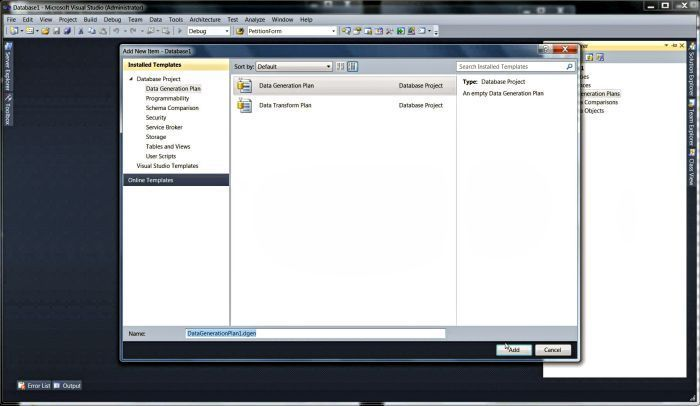
\includegraphics[width=\linewidth]{./figures/TrabalhosRelacionados/Visual-Studio.jpg}
			\label{fig:VSDG}
			\footnotesize Fonte: \cite{VSDataGenerator}.
		\end{figure}

		\emph{Test Data Generator} \cite{forgeDBDataGenerator} é uma ferramenta GUI (\emph{Graphical User Interface}) desenvolvida pela dbForge para gerar dados de teste para banco de dados SQL desde 1997.
		O software possui mais de duzentos geradores predifinidos e configuráveis, os quais permitem a geração de dados mais inteligentes, isto é, mais próximos da realidade, como nomes, localização, dados de saúde e afins.
		Quanto à compatibilidade, este é exclusivo do ecossistema Windows, com suporte ao \emph{Windows} 7, \emph{Windows Server} 2008, \emph{SQL Server Azure} 2008 ou versões superiores. 
		Além da GUI, também há o suporte para geração de dados a partir da linha de comando.
		O produto é distribuido sob licenças pagas e vitalícias, porém, com suporte ao cliente com tempo limitado e com trinta dias gratuitos para avaliação.
		\par
		Para usar o \emph{dbForge Test Data Generator}, é preciso fazer uma conexão com banco de dados. 
		A partir disso, utiliza-se os \emph{Data Generators} para determinar o comportamento dos dados para determinada coluna da tabela selecionada no Banco de dados.
		Os Geradores de dados podem ser do tipo \emph{Basics} e \emph{Advanced}. 
		Do primeiro tipo, são formas mais próximas dos dados primitivos, como datas, texto \emph{lorem ipsum}, JSON, \emph{ReGex}.
		Já o avançado conta com número de cartão de crédito, aniversário, número de conta bancária internacional, IPv4, \emph{hash} de senhas.  
		A geração de dados resume-se à população de banco de dados, não há uma forma de exportar os dados em arquivos como CSV e JSON.
		Ao acessar a documentação \cite{forgeDBDataGeneratorDoc} dos geradores, elas não estavam disponíveis (código HTTP 404), logo não foi encontrado mais informações inclusive sobre dados faltantes ou discrepantes.
		\par
		Há um suíte exclusivo para SQL Server, contudo também para Oracle, MySQL, PostgreSQL entre outros.
		Neste suíte, há várias ferramentas que auxiliam na manutenção, mas não, necessariamente, a geração de dados, a exemplo de um pre-visualizador de dados.
		Destes, pode-se citar um comparador de dados, criador de \emph{querys}, um monitor - para supervisão do banco de dados - e afins.
		\begin{figure}[h]
			\centering
			\caption{Usando o dbForge \emph{Test Data Generator}.}
			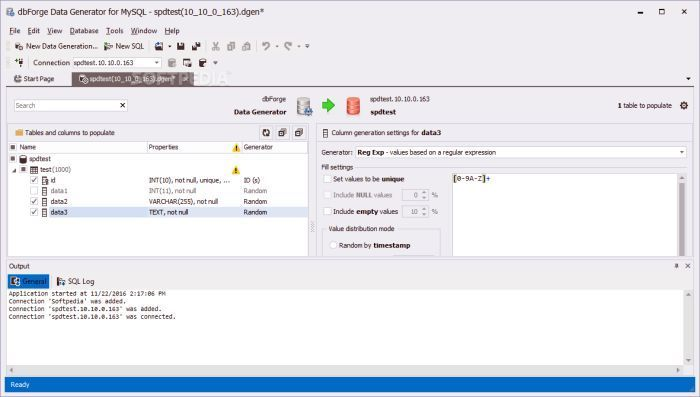
\includegraphics[width=\linewidth]{./figures/TrabalhosRelacionados/dbForge-Test-Data-Generator.jpg}
			\label{fig:dbForgeTDG}
			\footnotesize Fonte: \cite{forgeDBDataGenerator}.
		\end{figure}

		Mockaroo \cite{mockaroo} é um \emph{web site} e \emph{framework} para desenvolver dados de teste.
		Há um total de cento e quarenta e três geradores, sendo a maioria considerados geradores realistas.
		Por ser um site, é possível acessá-lo por qualquer sistema operacional, dependendo apenas de conexão com a internet.
		O produto possui versões gratuita e pagas. - \emph{Free}, \emph{Silver}, \emph{Gold}, \emph{Enterprise} as quais variam no \emph{host}, o qual pode ser do Mockaroo ou privado, máximo de registros por download, velocidade de download e preço.
		\par
		Na tela inicial, é possível escolher o nome da coluna, o tipo de gerador, entre outras opções.
		O campo \emph{blank} é possível determinar uma porcentagem de dados que ficarão em branco em ordem aleatória.
		Por conta da característica aleatória, o mecanismo de dados faltantes utilizado é o MCAR.
		\par
		Ao lado de \emph{blank} há o botão de fórmula, o qual é possível operar uma função com o valor gerado.
		Essas funções podem ser matemáticas ou outras disponibilizadas de acordo com a sintaxe de fórmula do Mockaroo.
		A partir dessa funcionalidade, é possível gerar dados discrepantes tanto ruidosos como anômalos, dependendo da função e parâmetros inseridos.
		\par
		Ainda na tela inicial encontra-se 
		 o botão para \emph{download} dos dados, 
		 pré-visualização dos mesmos, - sem gráficos, apenas tabular e CSV - 
		 algumas configurações como quantidade de linhas, 
		 formato dos dados para \emph{download}, 
		 botão para clone ou deleção de banco de dados, 
		 e importação de dados csv/Excel ou SQL.
		\par
		Outro serviço interessante da ferramenta é Mockaroo APIs \cite{mockarooAPI}.
		Este consiste em baixar dados programaticamente através de requisições REST (\emph{Representational State Transfer}).
		As requisições podem ser feitas de duas formas, a \emph{Generate API} - gera os dados através de um banco de dados salvo e os envia pelo corpo de uma requisição - 
		e \emph{Mock APIs} que simula um \emph{back-end} como tratamento de parâmetros e simulação de erros. 
		É pensado para desenvolvimento ágil de aplicações \emph{front-end}, isto é, sem perder muito tempo com o \emph{back-end} inicialmente.
		\begin{figure}[h]
			\centering
			\caption{Usando o Mockaroo.}
			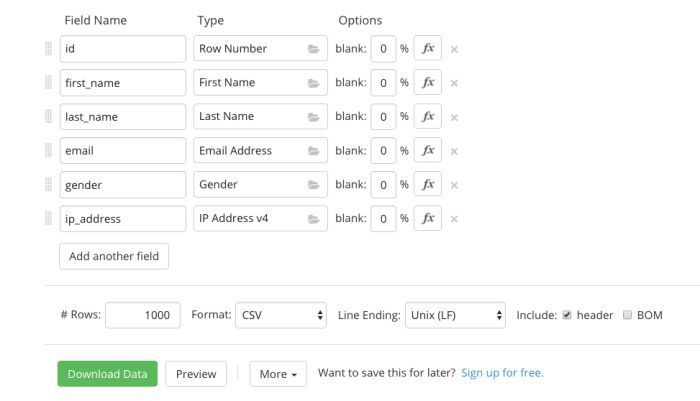
\includegraphics[width=\linewidth]{./figures/TrabalhosRelacionados/mockaroo.jpg}
			\label{fig:mockaroo}
			\footnotesize Fonte: \cite{mockaroo}.
		\end{figure}
		% \subsubsection{ApexSQL Generate}
		% \subsubsection{Datanamic Data Generator MultiDB}
		% \subsubsection{Upscene Advanced Data Generator}
		% \subsubsection{EMS Data Generator}
		% \subsubsection{GEDIS Studio}

		Na tabela \ref{table: aplicacoes relacionadas} é apresentada uma comparação de funcionalidades entre as aplicações estudadas.
		A dimensão B.D. diz respeito se a aplicação é capaz de se comunicar com um banco de dados para criar novas instâncias de dados.
		A dimensão Arquivo é referente à geração de dados e salvá-los em um arquivo.
		O suporte aos sistemas operacionais como Windows, Linux e MacOS é mostrado na dimensão S.O.
		O DTM possui suporte multiplataforma por meio da versão \emph{multiplatform runtime}, mas é limitada em relação à versão Windows.
		\par
		A dimensão D.F. e D.D. apresenta o suporte à geração de dados faltantes e dicrepantes, respectivamente.
		As instâncias que possuem sim* nessas dimensões significam que há suporte a geração de dados sintéticos e discrepantes, mas são feitos através de geradores personalizados, isto é, não há geradores predefinidos para esse fim.
		E o não* é porque a documentação sobre os geradores estava offline para consulta durante o desenvolvimento desse estudo.
		Quanto à dimensão Preço, esta refere-se ao acesso gratuito ou não a todas as funcionalidades da aplicação.
		O Gratuito* significa que há acesso gratuito, mas é limitado em processamento, havendo outras versões pagas.
		\begin{table}[h]
			\centering
			\caption{Tabela de comparação das funcionalidades de cada aplicação. 
				B.D. = Banco de Dados; 
				S.O. = Sistema Operacional; 
				D.F. = Dados Faltantes;
				D.D. = Dados Discrepantes;
				W.S. = \emph{Web Service}.}
			\vspace{0.5cm}
			\label{table: aplicacoes relacionadas}
			\begin{tabular}{r|lllllll}
			
				Nome                    & B.D. & Arquivo & S.O.    & D.F. & D.D. & W.S. & Preço    \\ % Note a separação de col. e a quebra de linhas
				\hline                                  % para uma linha horizontal
				\emph{Blocks}           & Não  & Sim     & Vários  & Sim  & Sim  & Sim & Gratuito \\ 
				\emph{DTM D.G.}         & Sim  & Sim     & Vários* & Não  & Sim* & Sim & Pago \\ 
				\emph{SQL D.G.}         & Sim  & Não     & Windows & Sim* & Sim* & Não & Pago \\ 
				\emph{MS Visual Studio} & Sim  & Não     & Vários  & Sim* & Sim* & Não & Pago \\ 
				\emph{Test D.G.}        & Sim  & Não     & Windows & Não* & Não* & Não & Pago \\ 
				\emph{Mockaroo}         & Não  & Sim     & Web     & Sim  & Sim  & Sim & Gratuito* \\ 

			\end{tabular}
			\bigskip
			\\
			\footnotesize Fonte: O autor do trabalho.
		\end{table}

		
	% ---
\chapter{Arquitetura do projeto}\label{cap_trabalho_academico}
% ---
	Em termos de organização do projeto, foi adotado o padrão de arquitetura de \emph{software} MVC (\emph{Model, View, Controller}), um modelo incremental de desenvolvimento, com reuniões diárias para discussão de problemas e melhorias, e utilização da ferramenta Trello \cite{trello} para organização e consistência das informações.
	\par
	Quanto ao desenvolvimento, foi utilizada a linguagem Javascript com foco para \emph{Desktop}, por meio da utilização do \emph{Framework Electron} \cite{electron}.
	Também foi adicionado o \emph{jQuery} para agilizar a codificação do projeto e o Node.js 10 \cite{nodejs} para acessar recursos do sistema operacional, para o desenvolvimento do \emph{Web Service} e também para dar suporte ao Electron.
	Do Javascript foi utilizado o Ecmascript 6 e seus novos recursos como o desenvolvimento assíncrono com as \emph{Promises} e \emph{arrow functions}.
	
	\section{Casos de uso do sistema}
		O diagrama de casos de uso visa demonstrar as diferentes formas de um usuário pode utilizar um sistema \cite{UCdefinition}.
		Por conta disso, é utilizado o Diagrama de Casos de Uso para demonstrar as principais funcionalidades do sistema Blocks.
		Na figura \ref{fig:diagramaUC} são encontrados um total de dez casos de uso, nomeados de UC01 a UC10.
		\begin{figure}[h!]
			\centering
			\caption{Diagrama de Caso de uso do Blocks}
			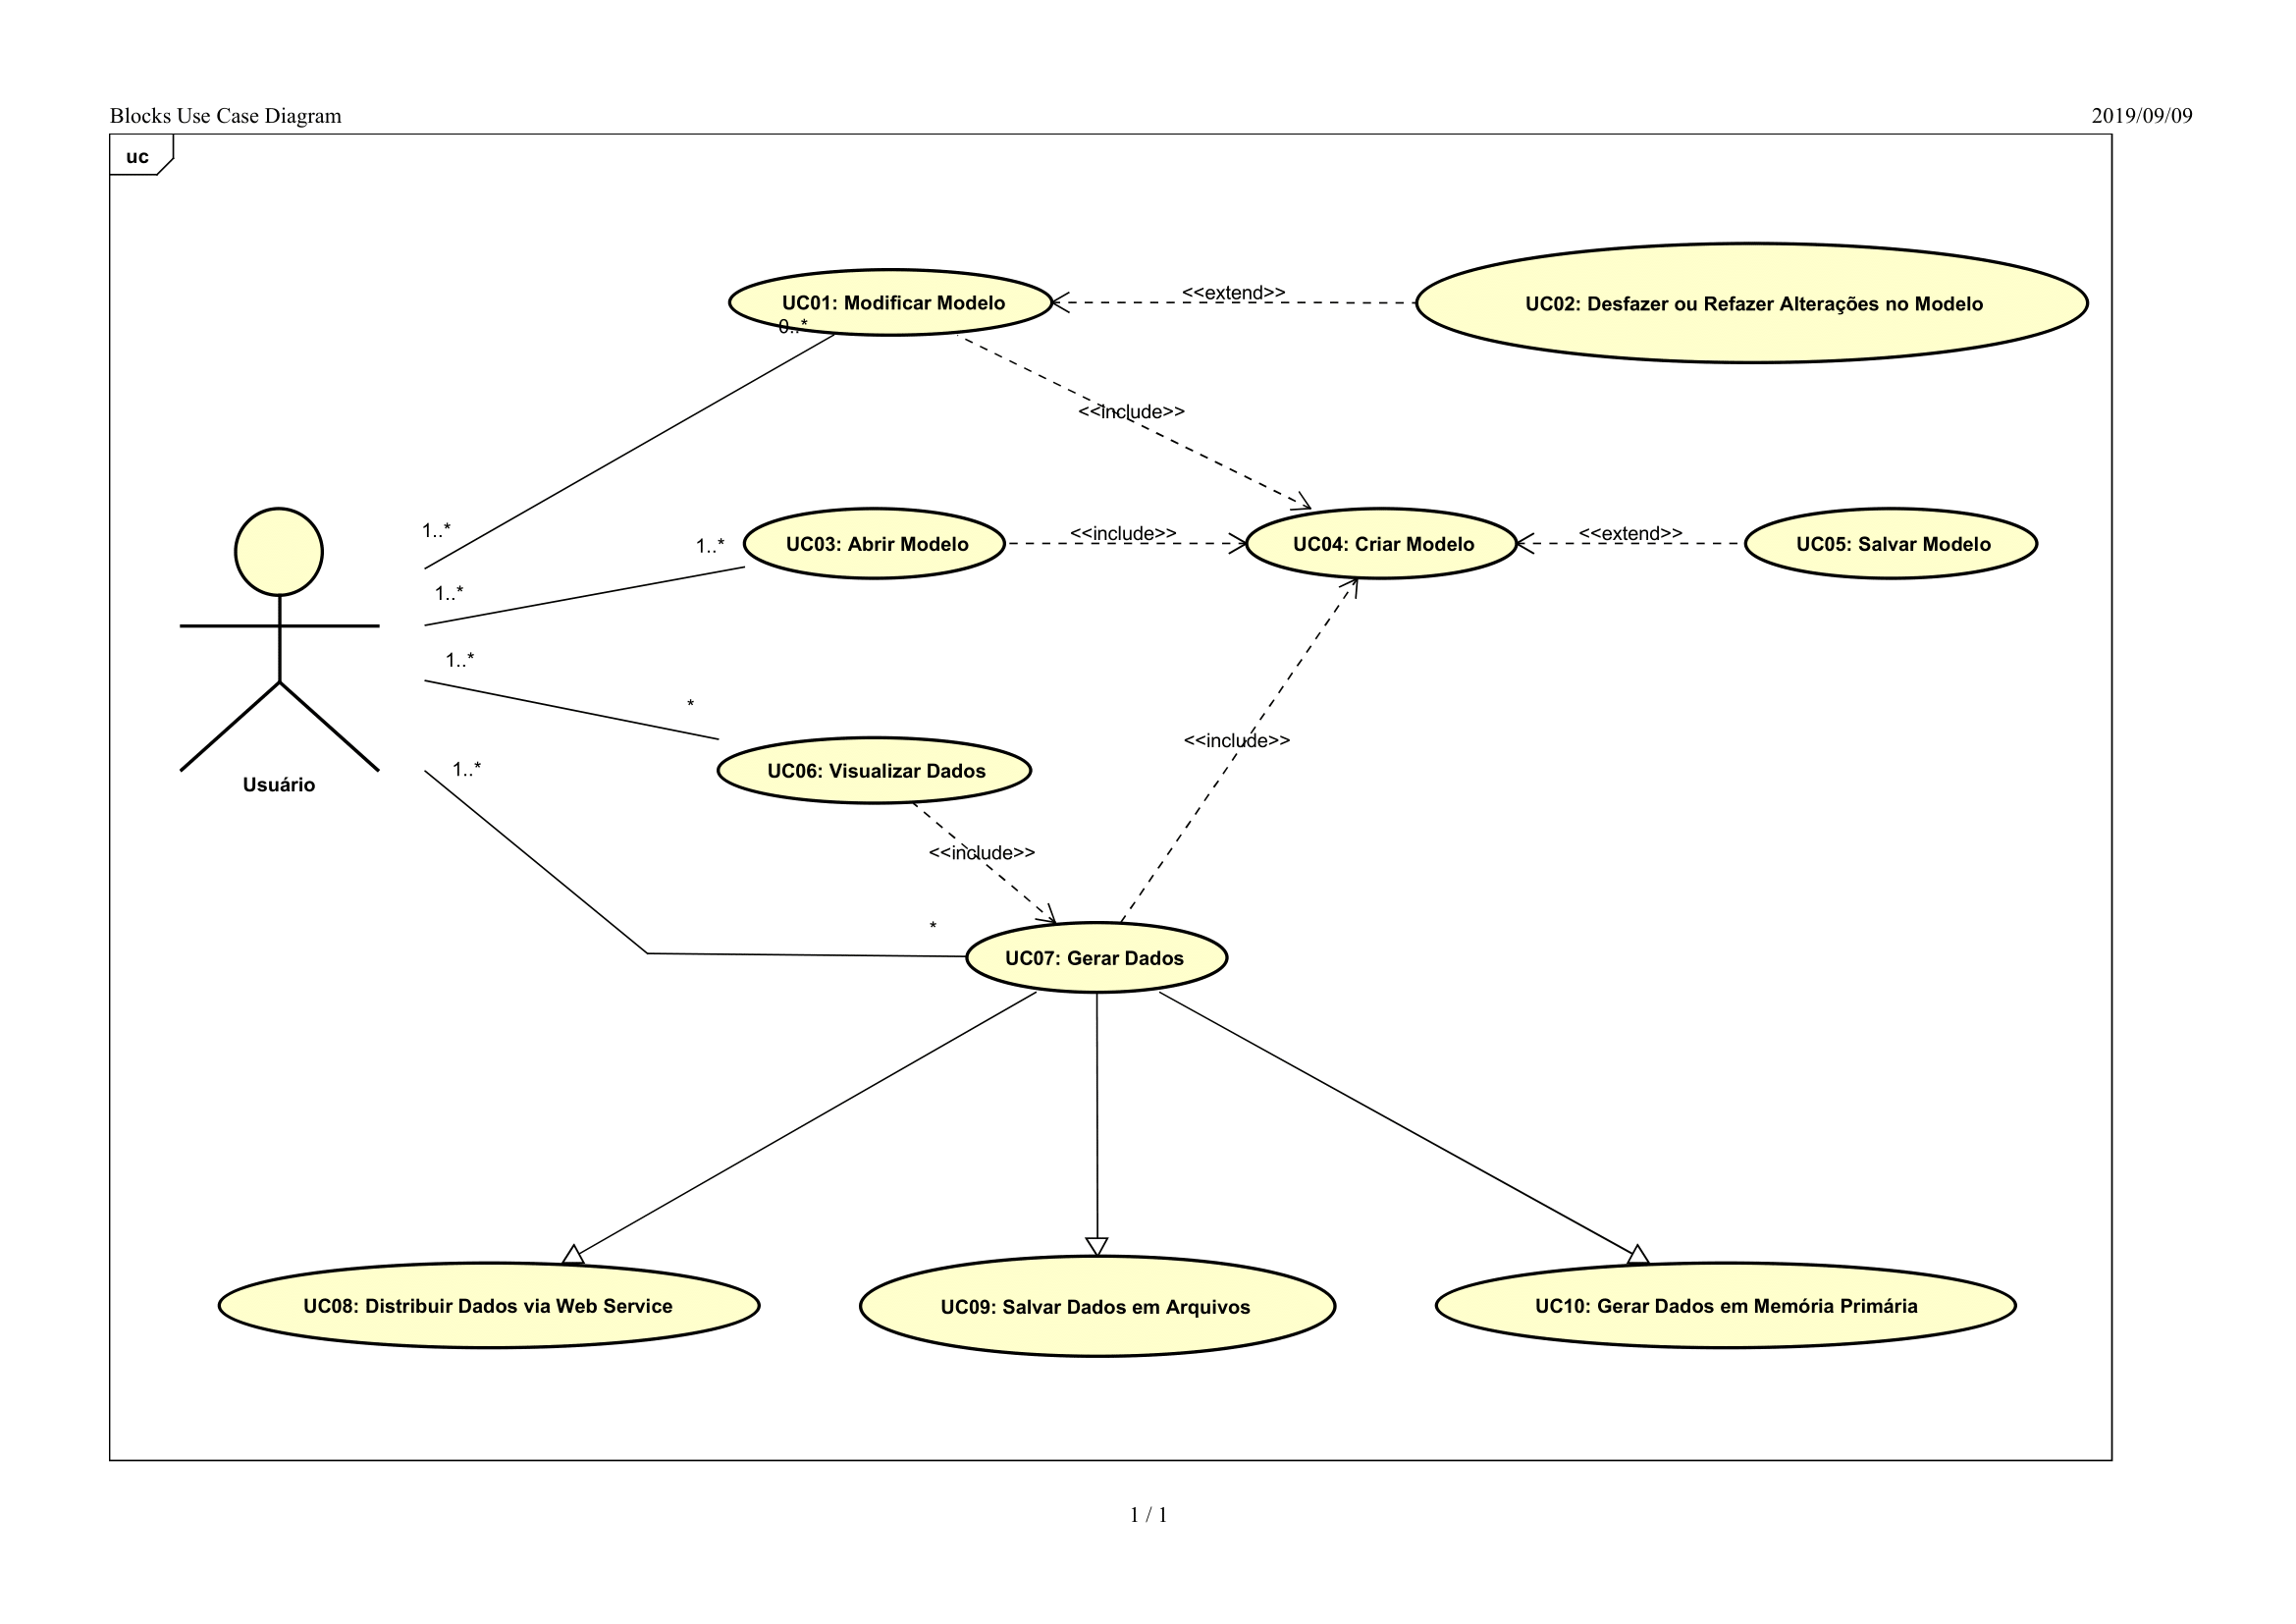
\includegraphics[width=\linewidth]{./figures/prototipo/diagramaUC.png}
			\label{fig:diagramaUC}
			\footnotesize Fonte: O autor do trabalho.
		\end{figure}
		\par
		No UC01 mostra que é possível modificar um modelo, isto é, adicionar ou remover dimensões, alterar geradores e afins; também há inclusão do UC04 e a possibilidade de desfazer ou refazer as alterações (UC02).
		O UC04 representa a criação do modelo.
		Outros casos de uso que possuem relação com UC04 é o UC03 e UC07 como inclusão e UC05 como extensão.
		\par
		UC03 é uma funcionalidade para reaproveitamento do modelo, também está ligado à validação de teste por outros pesquisadores.
		UC07 é o principal caso de uso do Blocks, o qual refere-se à geração de dados, progredindo para o \emph{Big Data} ou não.
		Esta geração pode ser feita, especificamente, de três formas: gerando dados em memória, para ser utilizado dentro do sistema (UC10);
			salvar em arquivos - TSV, CSV e JSON - (UC09);
			e distribuir os dados através de requisições HTTP (UC08).
		\par
		Incluindo a UC07, mais especificamente a UC10, a UC06 permite que o usuário visualize os dados. 
		Assim, a visualização pode ser rápida (\emph{preview}) ou detalhada (\emph{VisApplication}), tendo um panorama do comportamento dos dados. 
		Com isso, pode-se validar os dados, ter \emph{insights} para aprimorar o modelo e afins.
	\section{Diagrama de Classes}
	No diagrama de classes visto na figura \ref{fig:diagramaCD} é possível encontrar a estrutura da classe geradores de forma resumida.
	Há uma classe abstrata chamada \emph{Generator} que possui a maioria dos métodos e atributos, sendo que alguns deles são sobrescritos nas subclasses.
	Na segunda geração de classes (ver figura \ref{fig:diagramaCDCima}), elas existem para identificar as categorias - exceto \emph{Real Data Wrapper} e não adicionam novas propriedades - com exceção da classe \emph{Sequence}, por exemplo.
	Então a terceira geração de classes (ver figura \ref{fig:diagramaCDBaixo}) são os geradores em si, que herdam das suas respectivas categorias, mas uma exceção é a classe \emph{SwitchCaseFunction} a qual possui a propriedade de permitir geradores distintos de acordo com o valor.
	\begin{figure}[h!]
		\centering
		\caption{Diagrama de Classes dos geradores do Blocks.}
		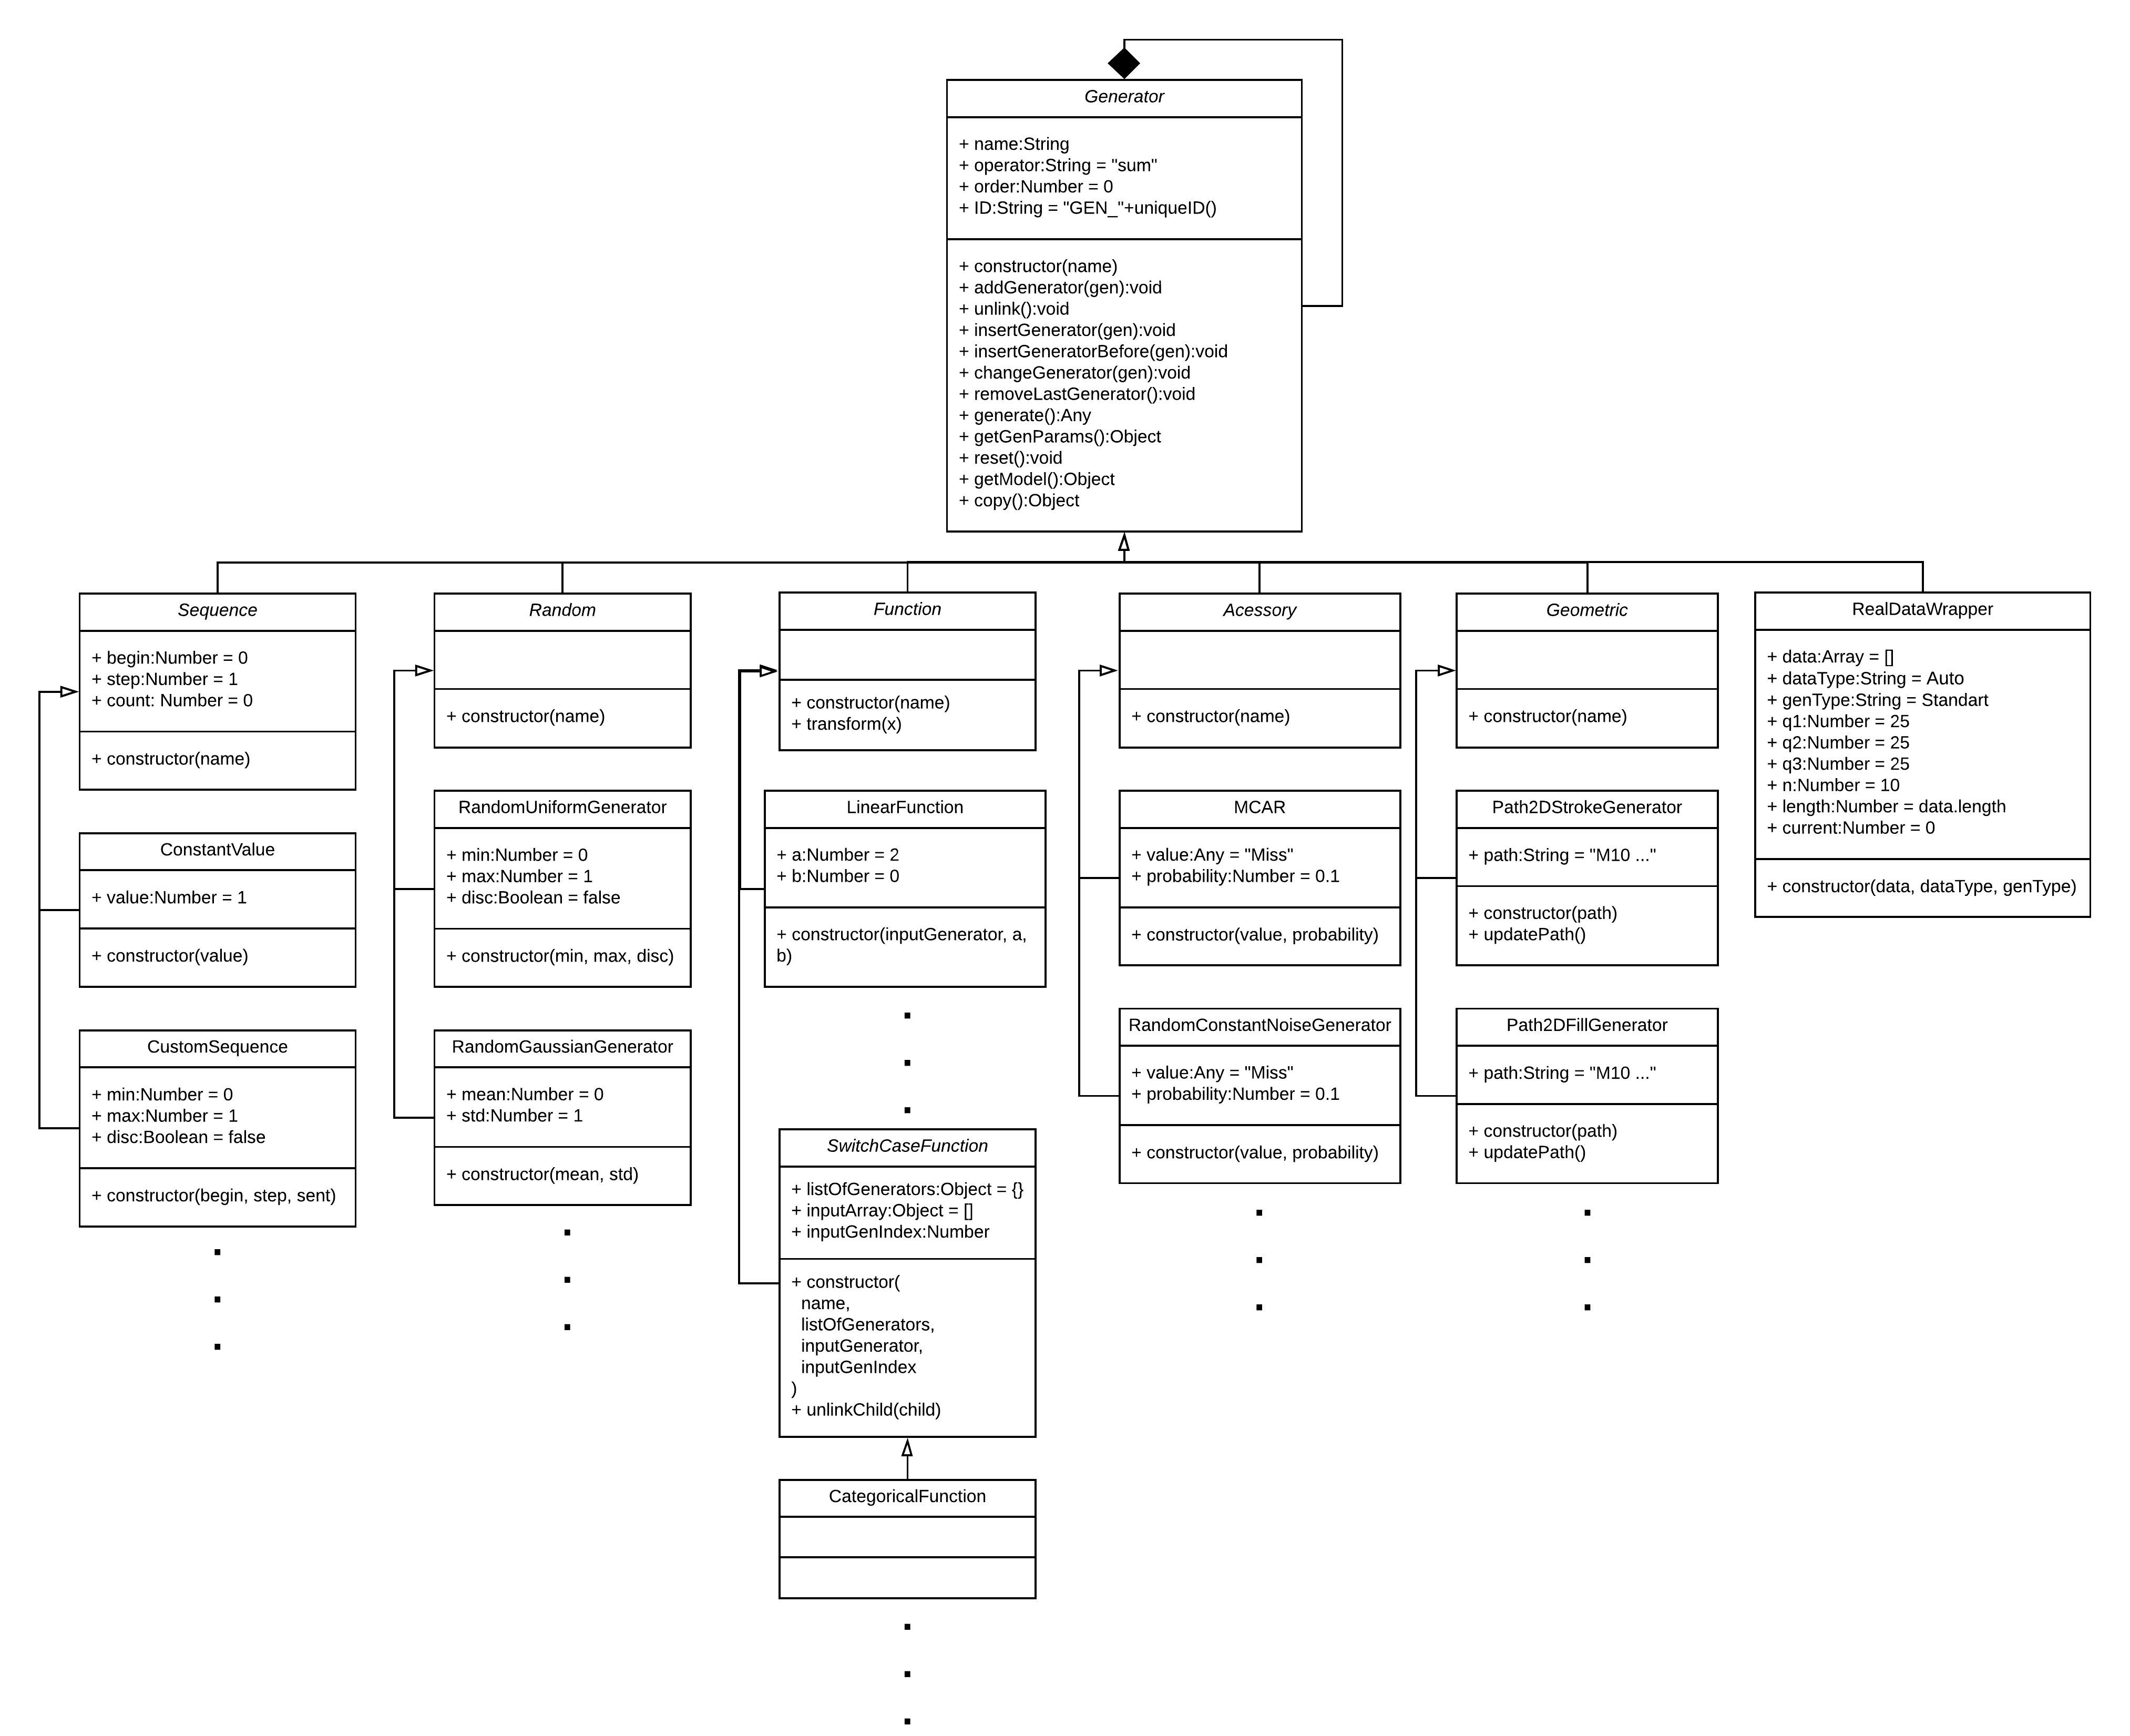
\includegraphics[width=\linewidth]{./figures/prototipo/DiagramadeClasseGeradores.png}
		\label{fig:diagramaCD}
		\footnotesize Fonte: O autor do trabalho.
	\end{figure}
	
	\begin{figure}[h!]
		\centering
		\caption{Diagrama de Classes (2ª Geração) dos geradores do Blocks.}
		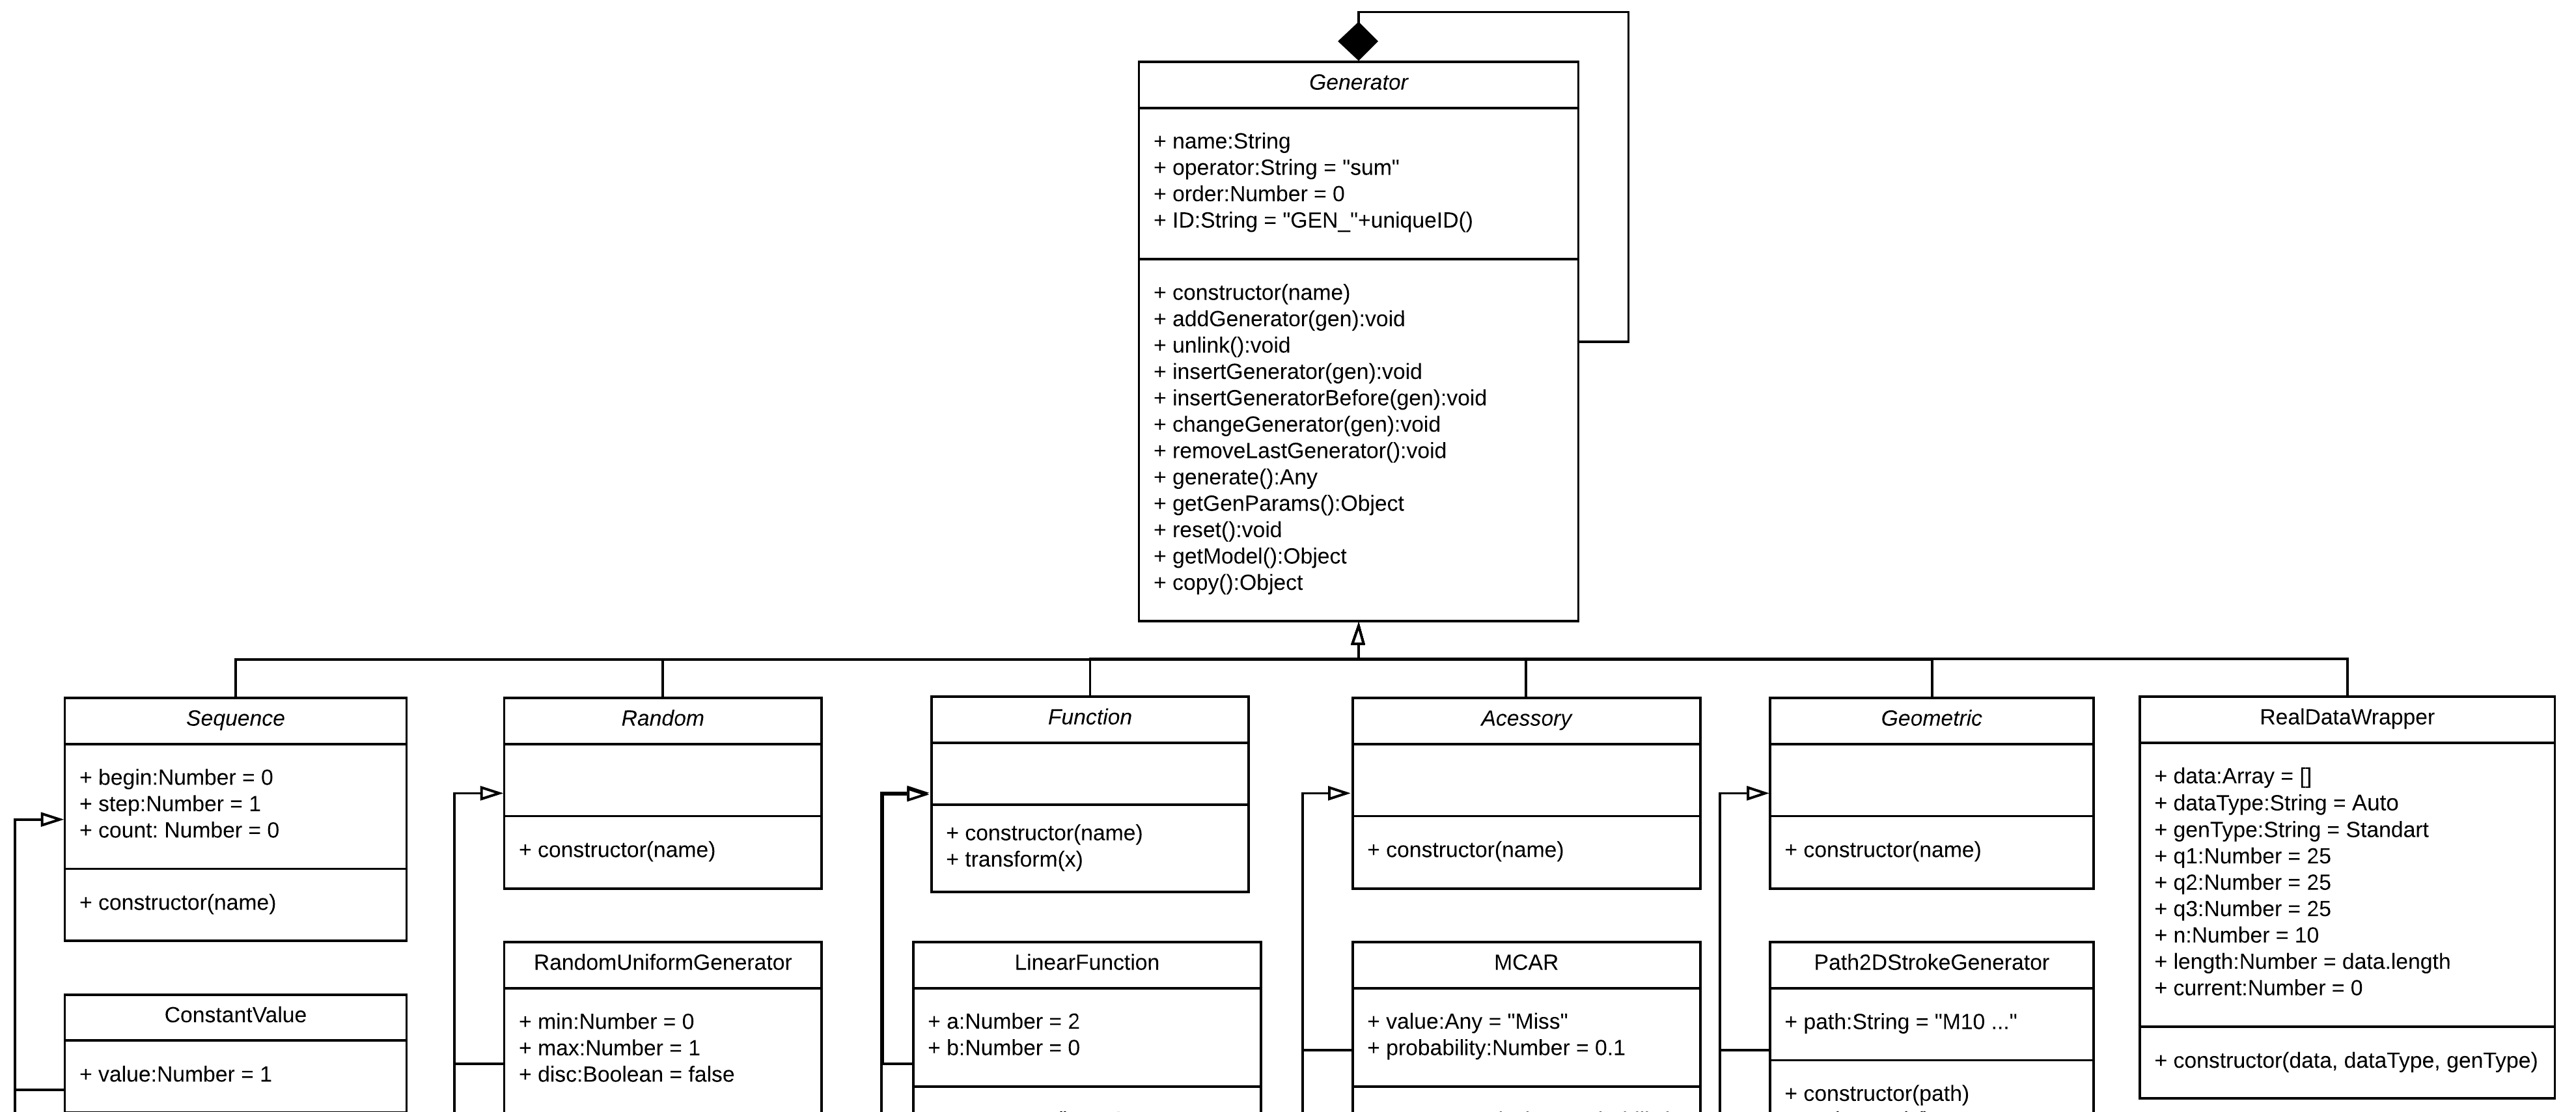
\includegraphics[width=\linewidth]{./figures/prototipo/DiagramadeClasseGeradoresCima.png}
		\label{fig:diagramaCDCima}
		\footnotesize Fonte: O autor do trabalho.
	\end{figure}

	\begin{figure}[h!]
		\centering
		\caption{Diagrama de Classes (3ª Geração) dos geradores do Blocks.}
		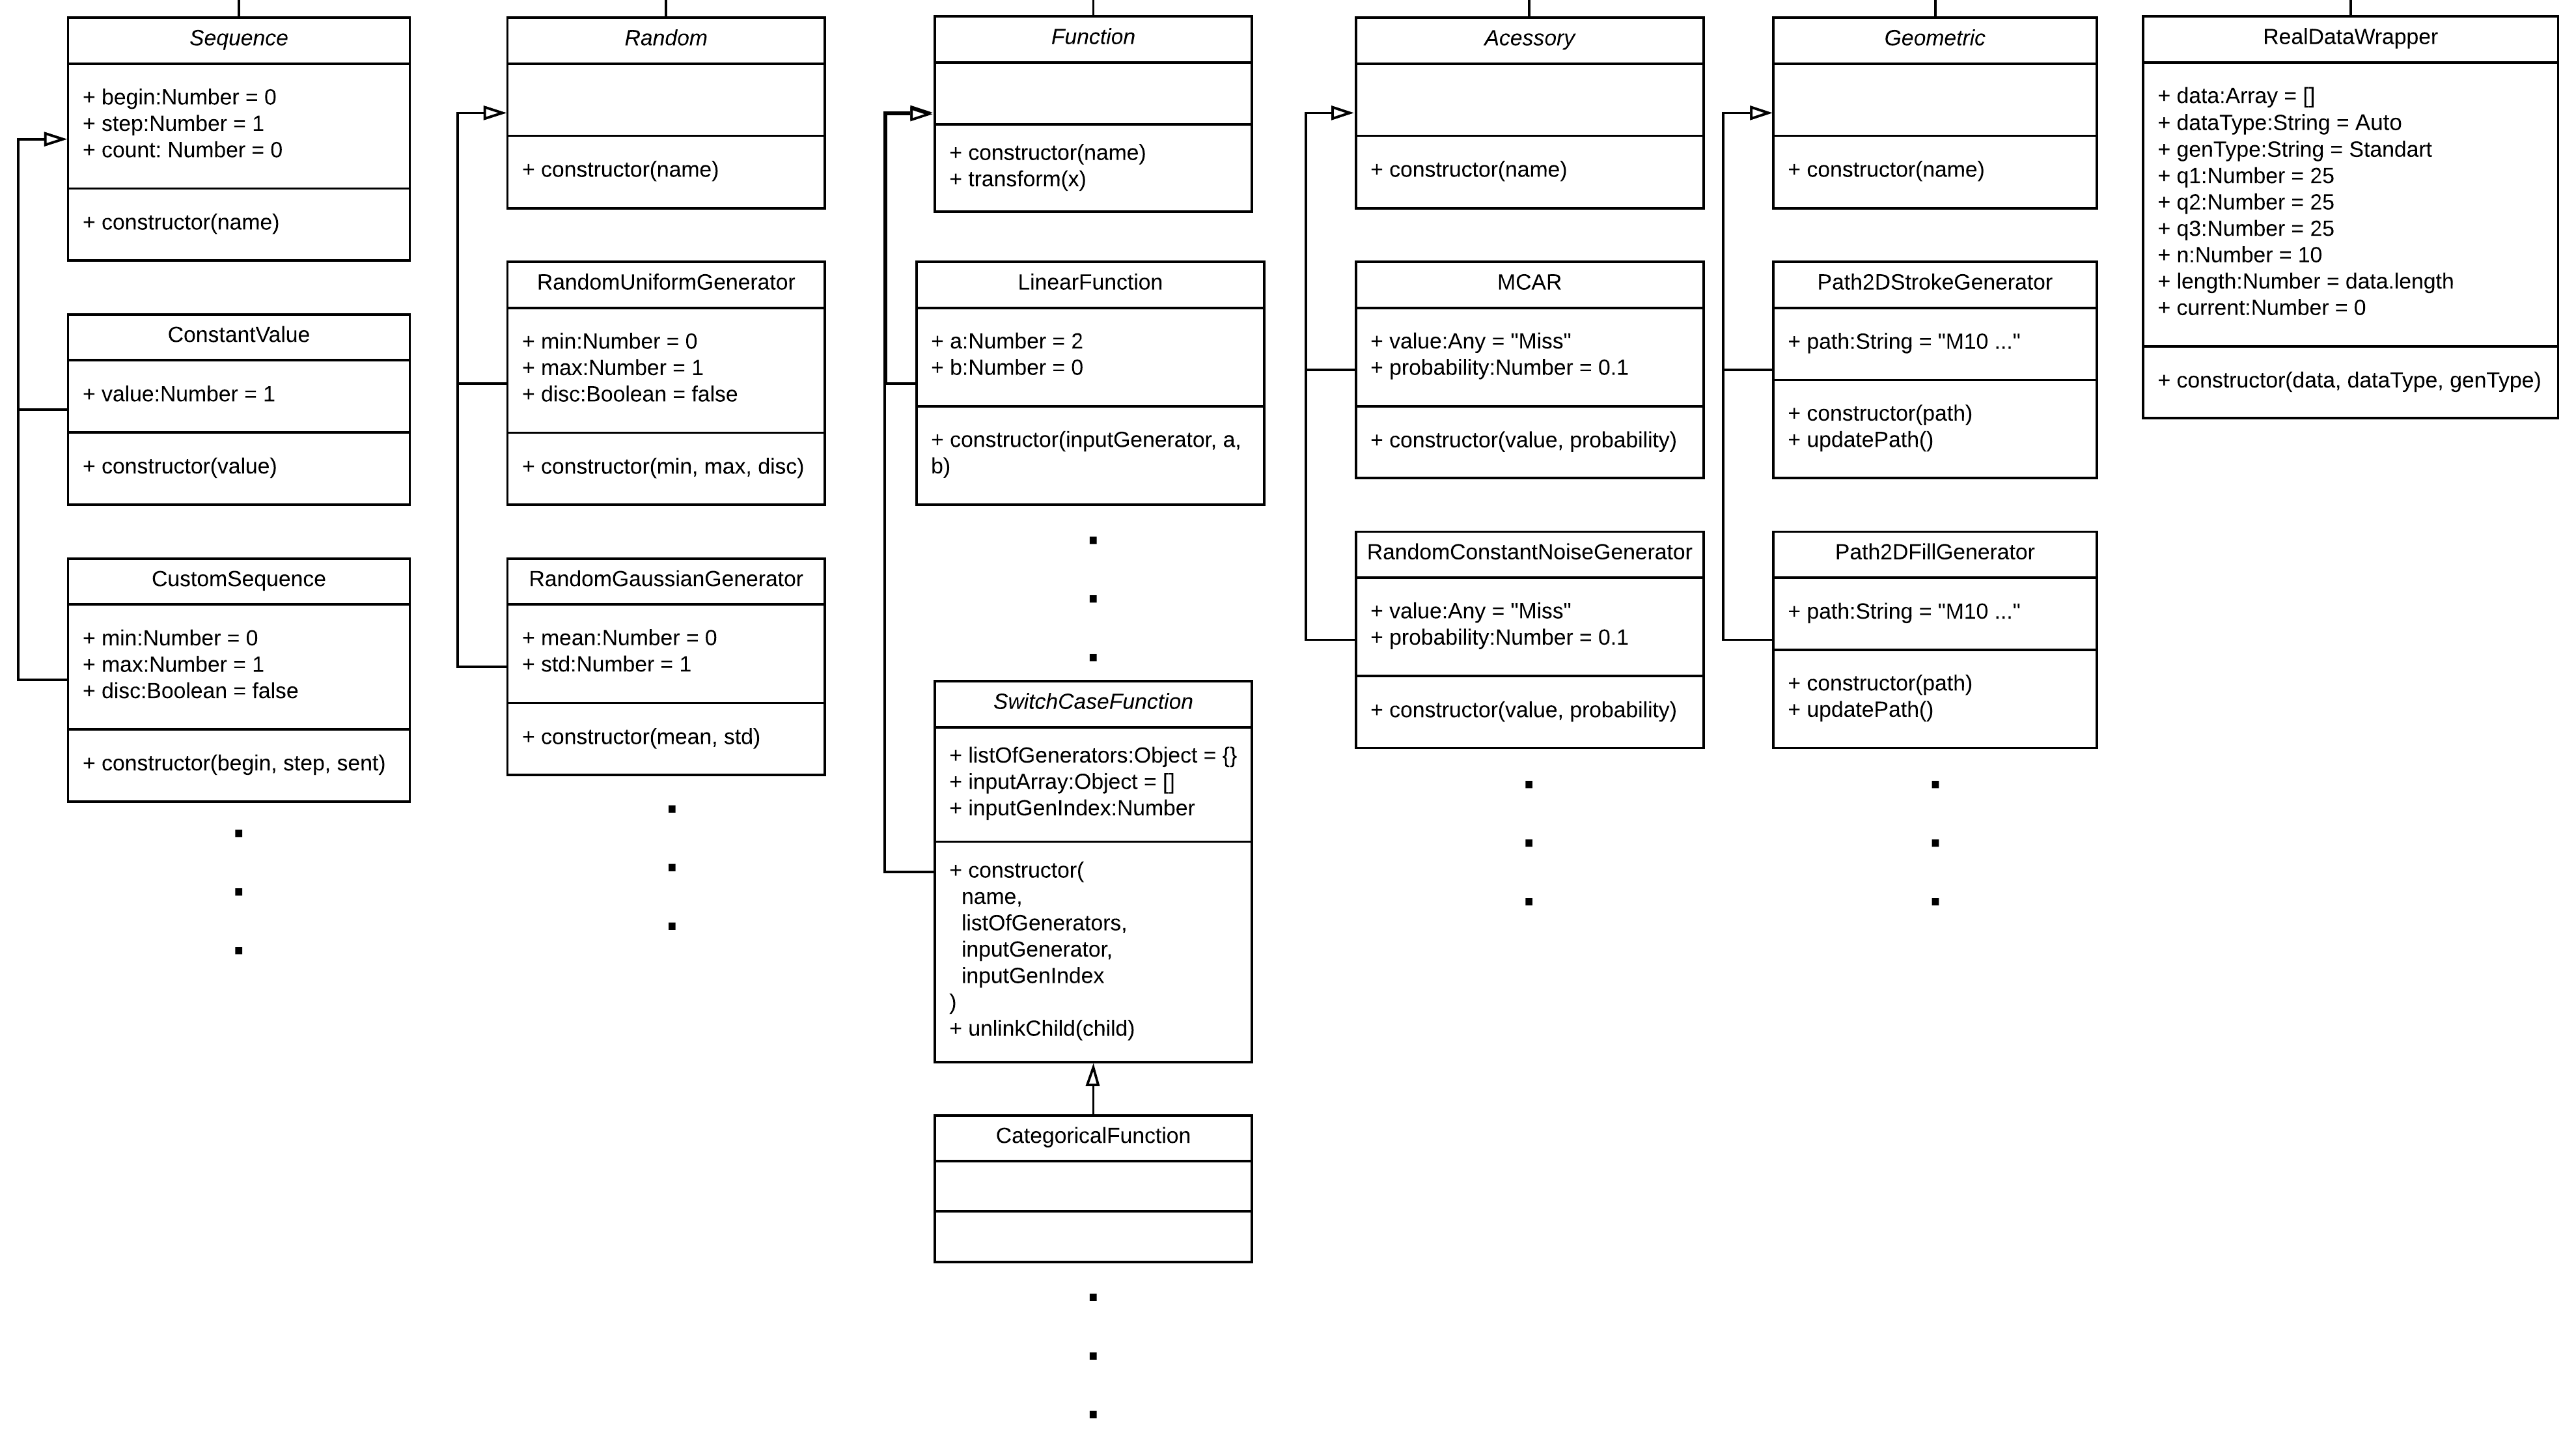
\includegraphics[width=\linewidth]{./figures/prototipo/DiagramadeClasseGeradoresBaixo.png}
		\label{fig:diagramaCDBaixo}
		\footnotesize Fonte: O autor do trabalho.
	\end{figure}

	\pagebreak
	\section{Diagrama de Sequência de atividades no Blocks}
	Para gerar os diagramas de sequência do Blocks, foram utilizados os casos de uso UC06 e UC09, vistos na figura \ref{fig:diagramaUC}.
	No diagrama \ref{fig:DiagramadeSequenciaArquivo} percebe-se que há a introdução das configurações do modelo pelo usuário, então o sistema cria/modifica o objeto modelo (UC01).
	Mais abaixo, há 2 loops para geração dos dados, o primeiro é a geração pelos geradores presentes no modelo até um certo limite, então esse conjunto de dados é salvo no arquivo e em seguida há uma resposta ao usuário de que houve progresso.
	\begin{figure}[h!]
		\centering
		\caption{Diagrama de Sequência para geração de dados em arquivos no Blocks.}
		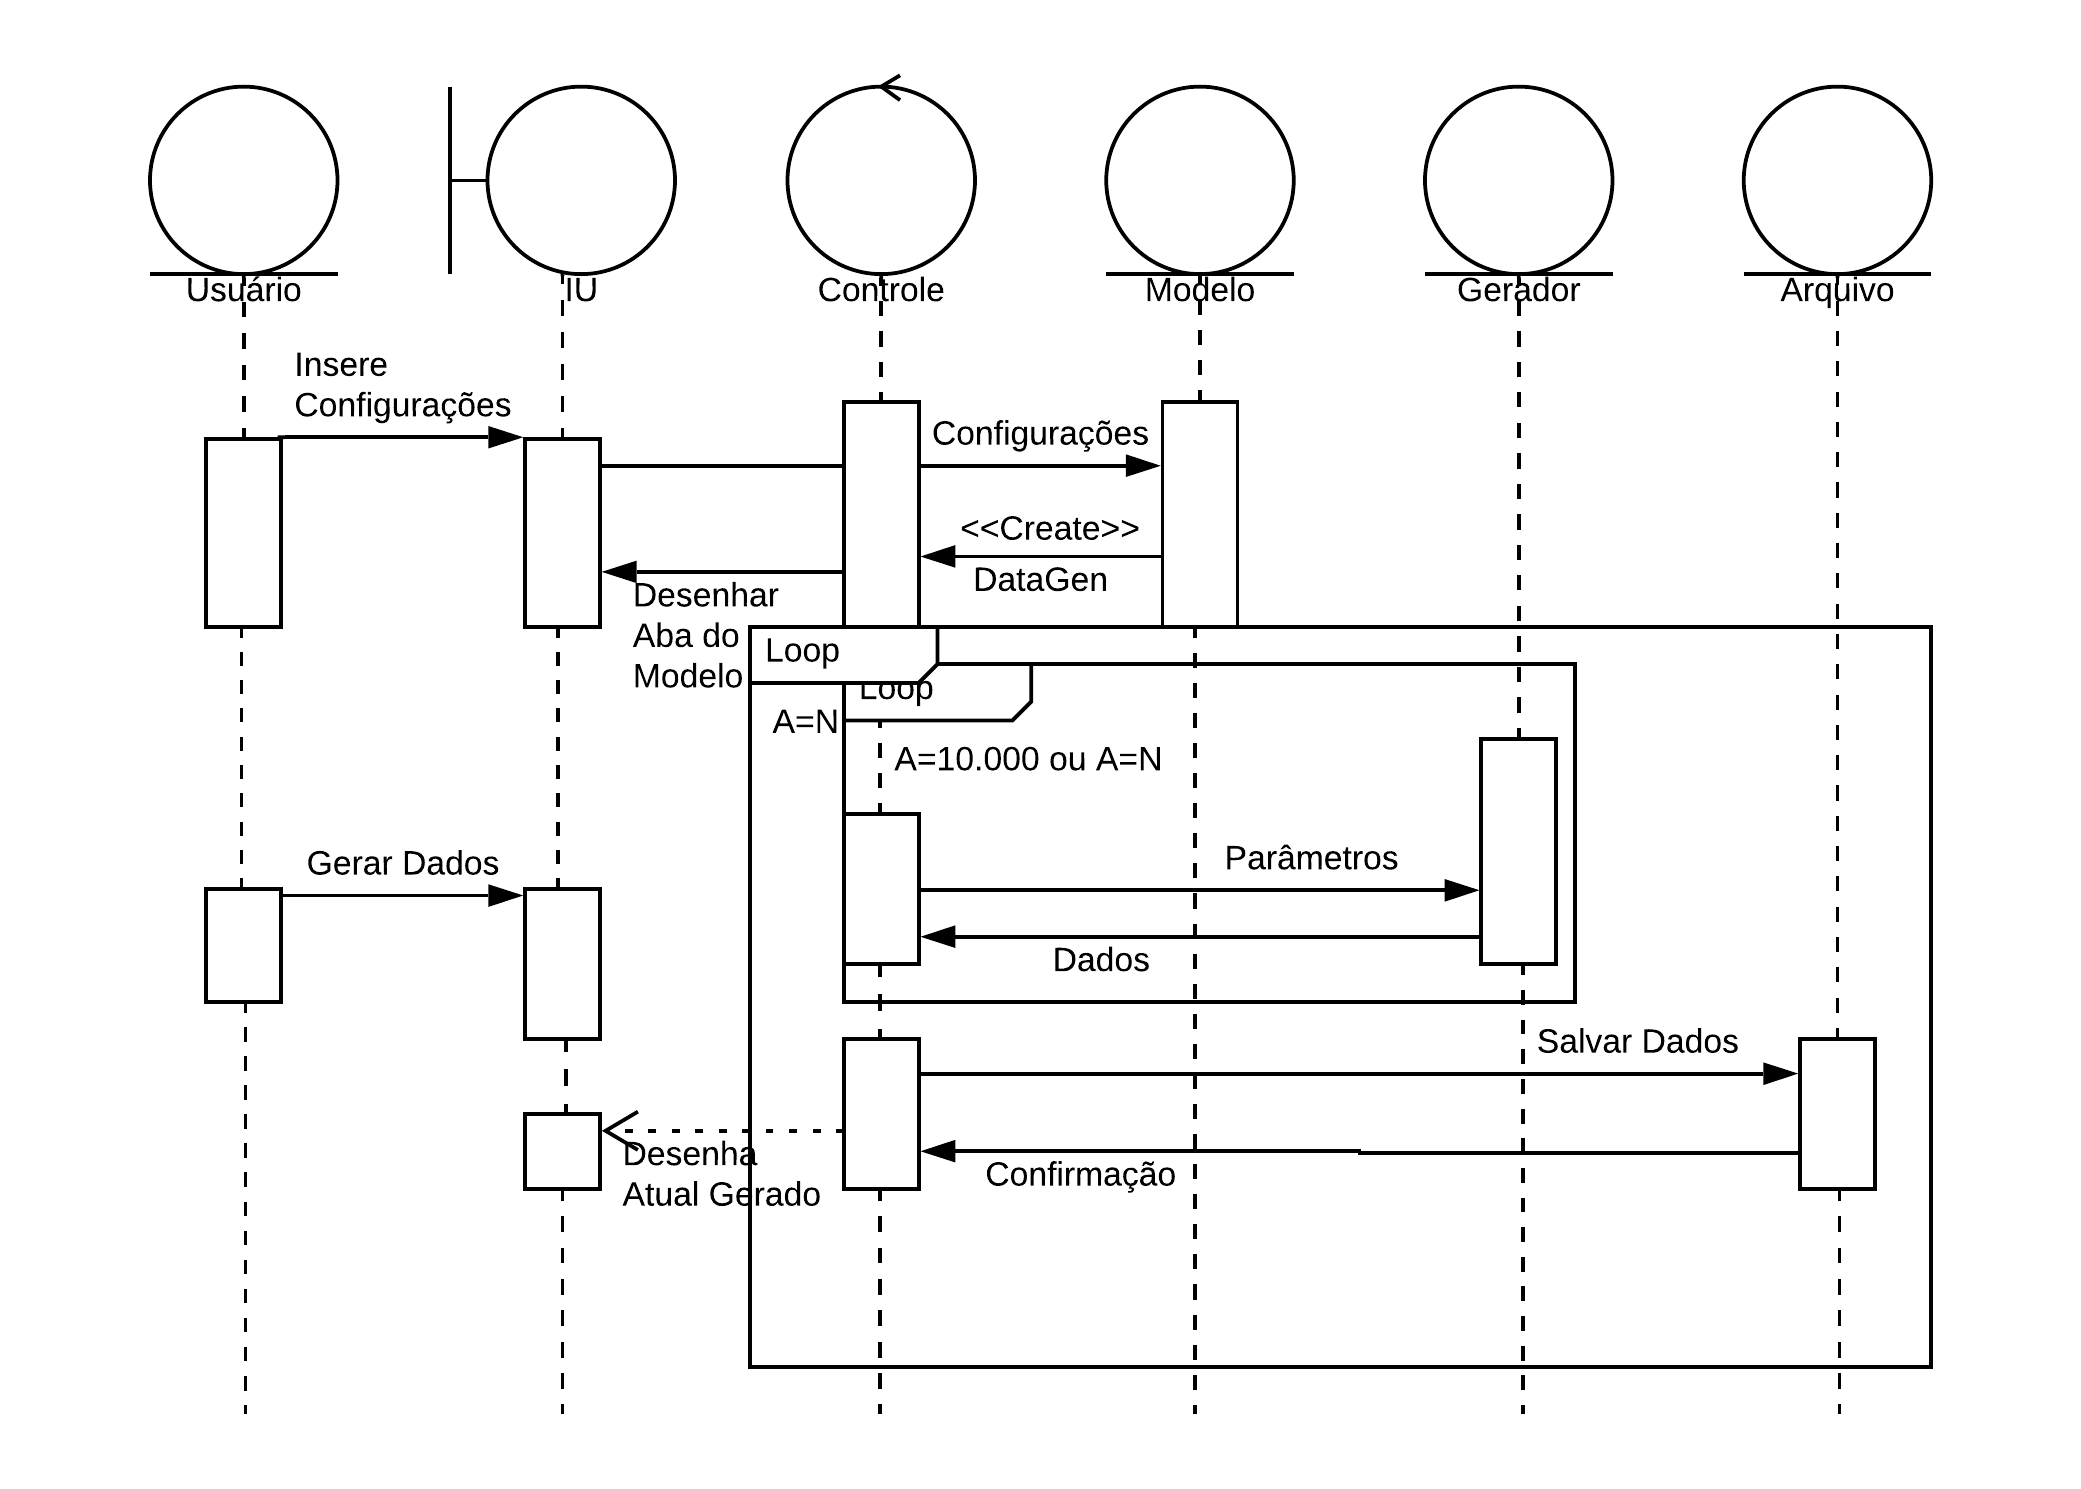
\includegraphics[width=\linewidth]{./figures/prototipo/DiagramadeSequenciaArquivo.png}
		\label{fig:DiagramadeSequenciaArquivo}
		\footnotesize Fonte: O autor do trabalho.
	\end{figure}
	\par
	No diagrama de sequência visto na figura \ref{fig:DiagramadeSequenciaVisApplication} é em relação ao UC06.
	Primeiramente, assim como na geração do arquivo, há o uso do UC01.
	Em seguida há geração dos dados em memória referente ao UC10.
	Com esses dados em memória, o \emph{preview} é desenhado automaticamente.
	A partir dos dados, há uma comunicação via \emph{WebSocket} com o VisApplication enviando os dados.
	O VisApplication retorna as opções de visualização, o usuário escolhe uma e então é retornado a visualização para que esta seja renderizada.

	\begin{figure}[h!]
		\centering
		\caption{Diagrama de Sequência para visualização de dados no Blocks.}
		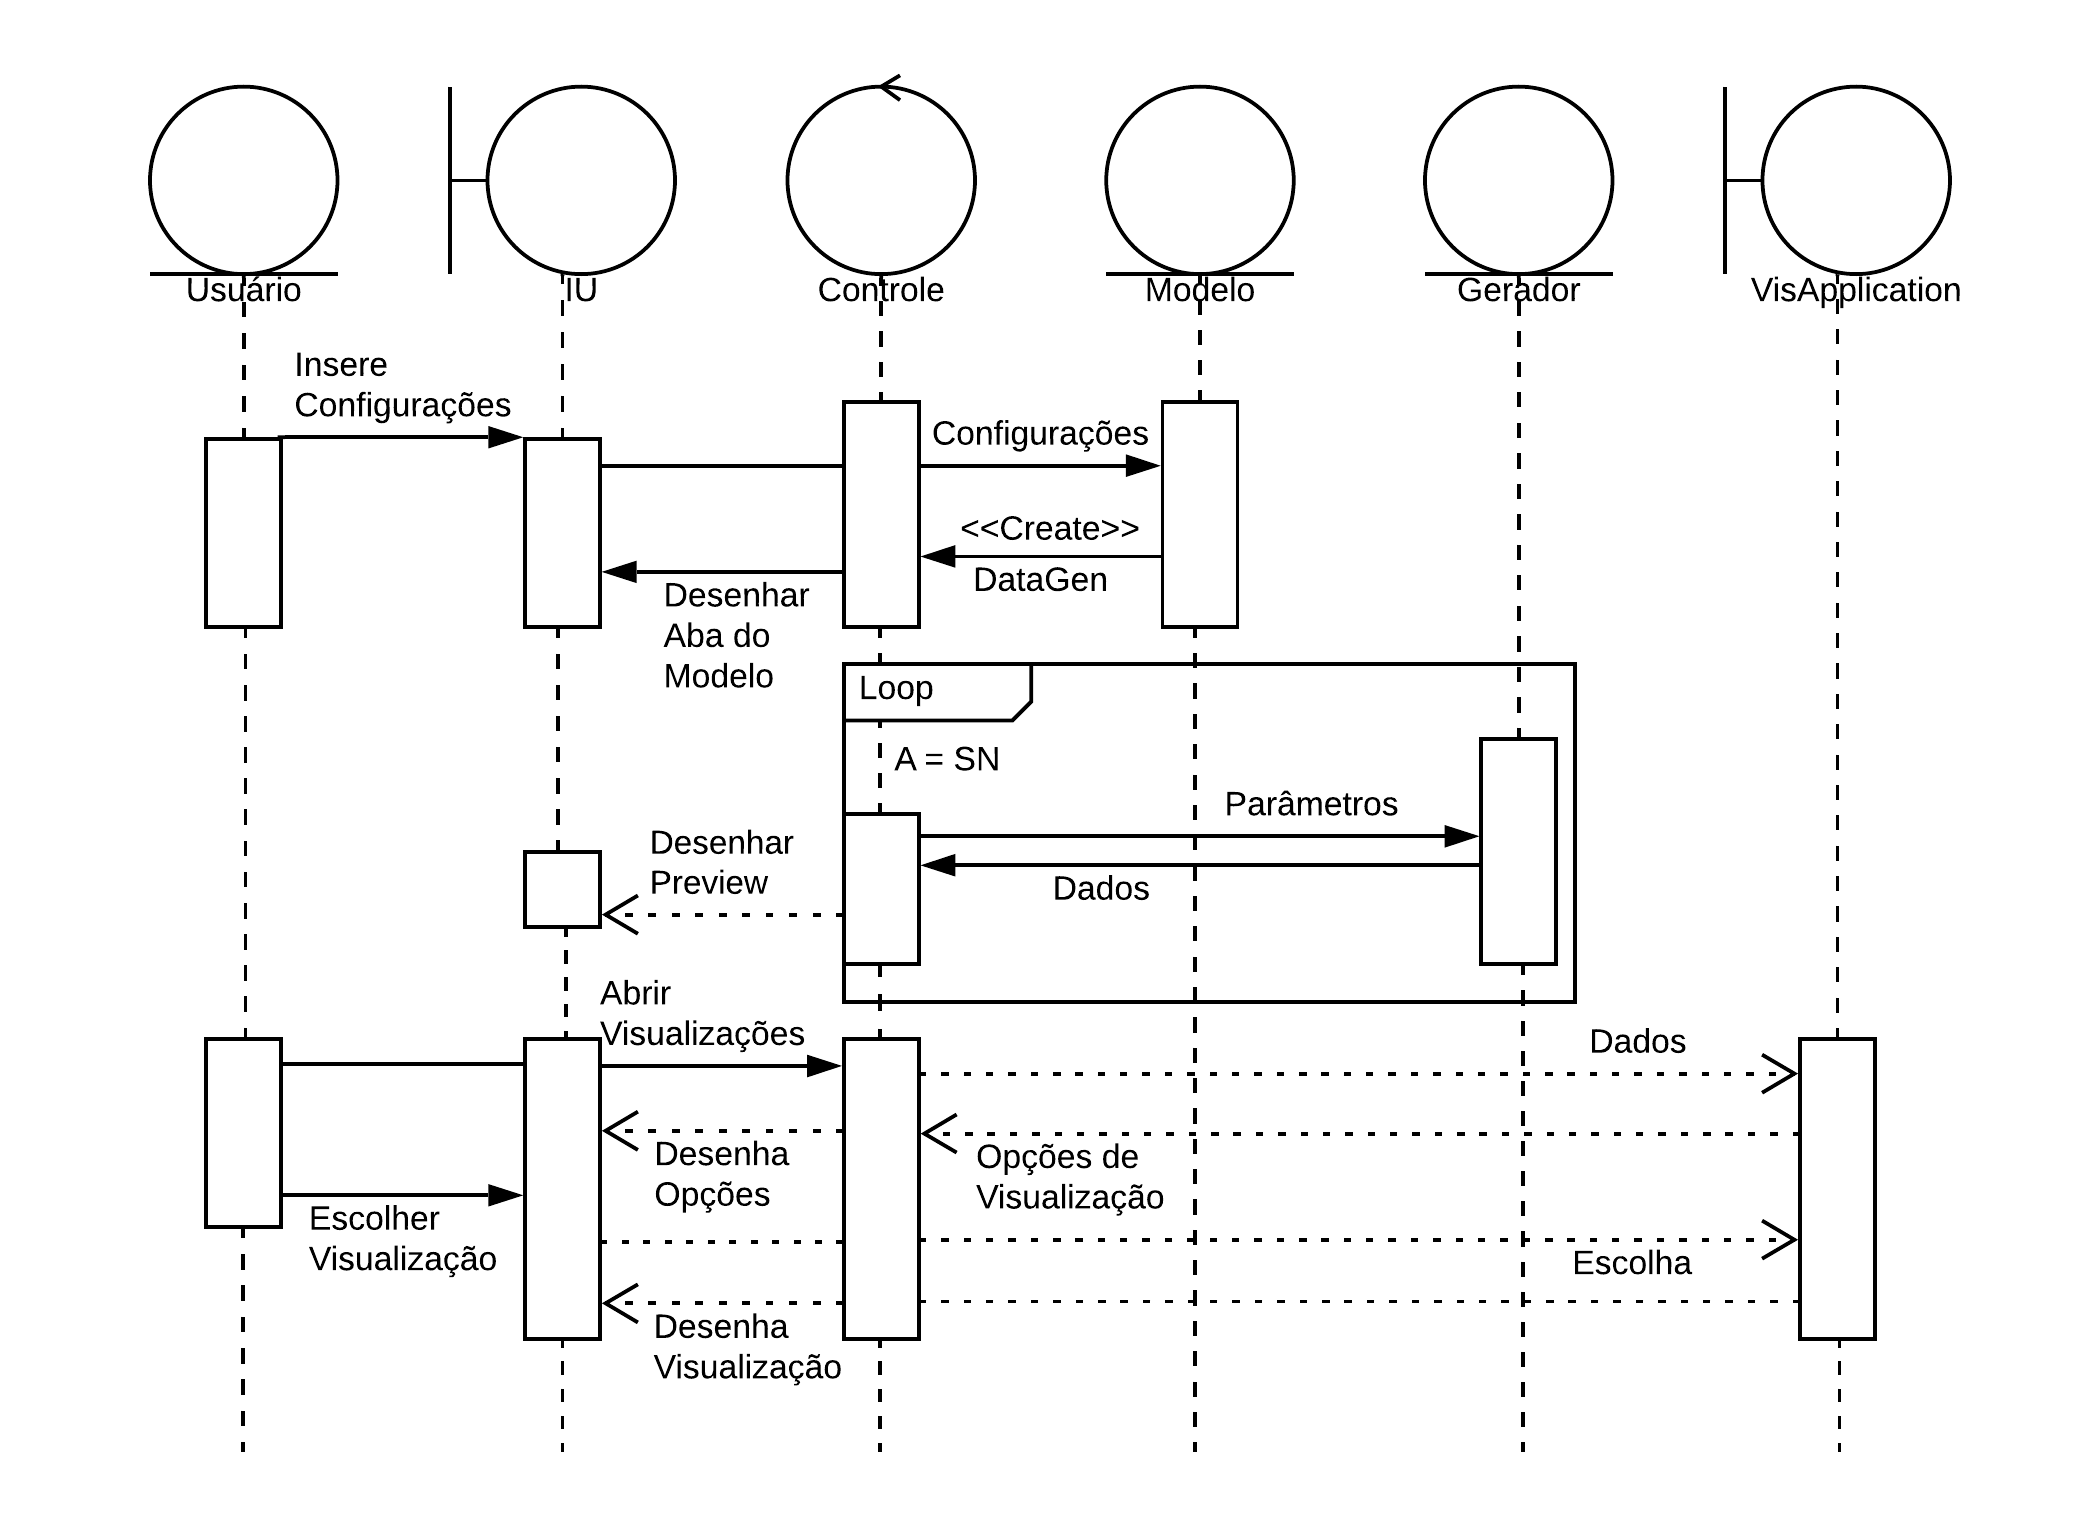
\includegraphics[width=\linewidth]{./figures/prototipo/DiagramadeSequenciaVisApplication.png}
		\label{fig:DiagramadeSequenciaVisApplication}
		\footnotesize Fonte: O autor do trabalho.
	\end{figure}
	\pagebreak
	\section{Pseudocódigos dos geradores desenvolvidos}
		São apresentados pseudocódigos nessa seção com o objetivo de demonstrar como foram implementados os métodos para gerar dados sintéticos e discrepantes.
		Primeiramente é mostrada a classe Generator (ver figura \ref{fig:Generator}), que utiliza o padrão de projeto \emph{Decorator} com o fim de encadear os geradores.
		Nessa clase estão os principais atributos como o nome do gerador, os geradores encadeados (gerador), um operador (soma, subtração, divisão etc) entre outros.
		Quanto ao método gerar, este verifica se há um gerador encadeado, se não ele retorna o valor recebido.
		Por ser uma classe abstrata, a classe Generator recebe o valor da subclasse instanciada.
		%TODO: Generator
		\begin{figure}[h!]
			\centering
			\caption{Pseudocódigo sobre a classe Generator do Blocks.}
			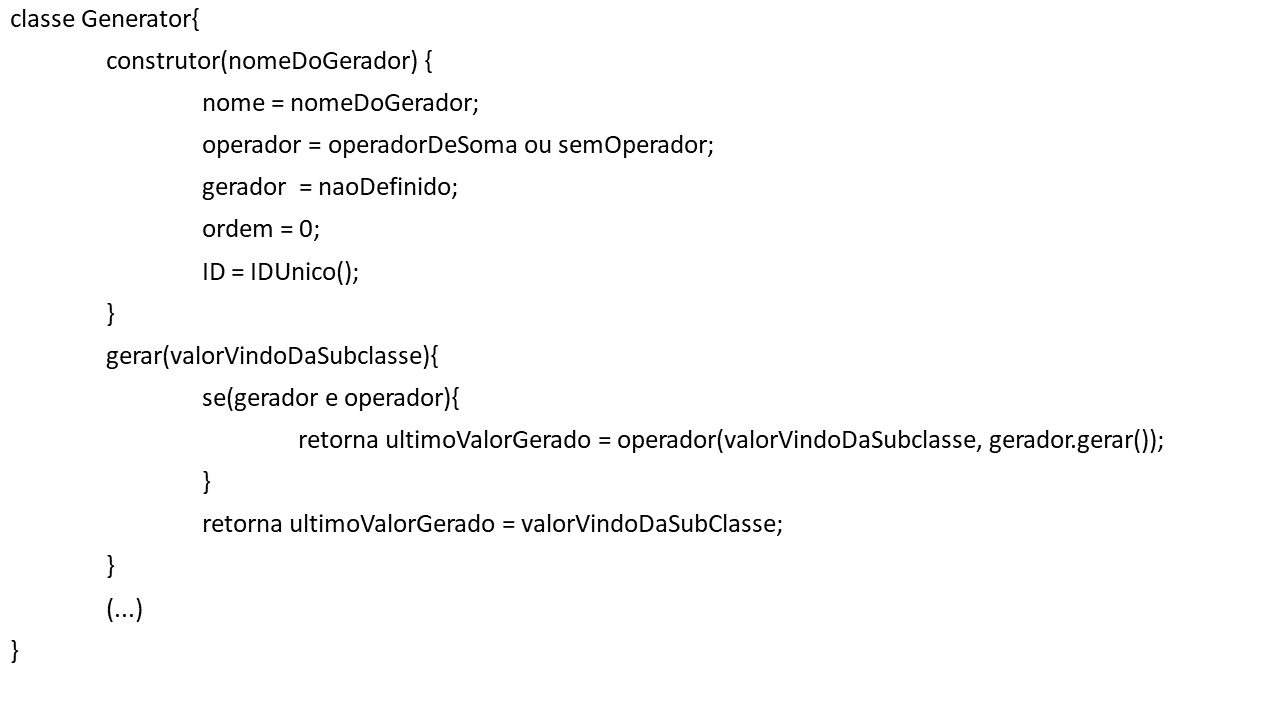
\includegraphics[width=\linewidth]{./figures/prototipo/Generator.png}
			\label{fig:Generator}
			\footnotesize Fonte: O autor do trabalho.
		\end{figure}
		\par
		%TODO: MCAR
		O gerador MCAR (ver classe na figura \ref{fig:classeMCAR}) tem como atributos um valor (o dado faltante recebe esse valor) e uma probabilidade, isto é, uma taxa aproximada de dados faltantes nessa dimensão.
		Para gerar, ele verifica a probabilidade e então retorna o valor faltante, se não o valor do gerador encadeado.
		
		\begin{figure}[h!]
			\centering
			\caption{Pseudocódigo sobre a classe MCAR do Blocks.}
			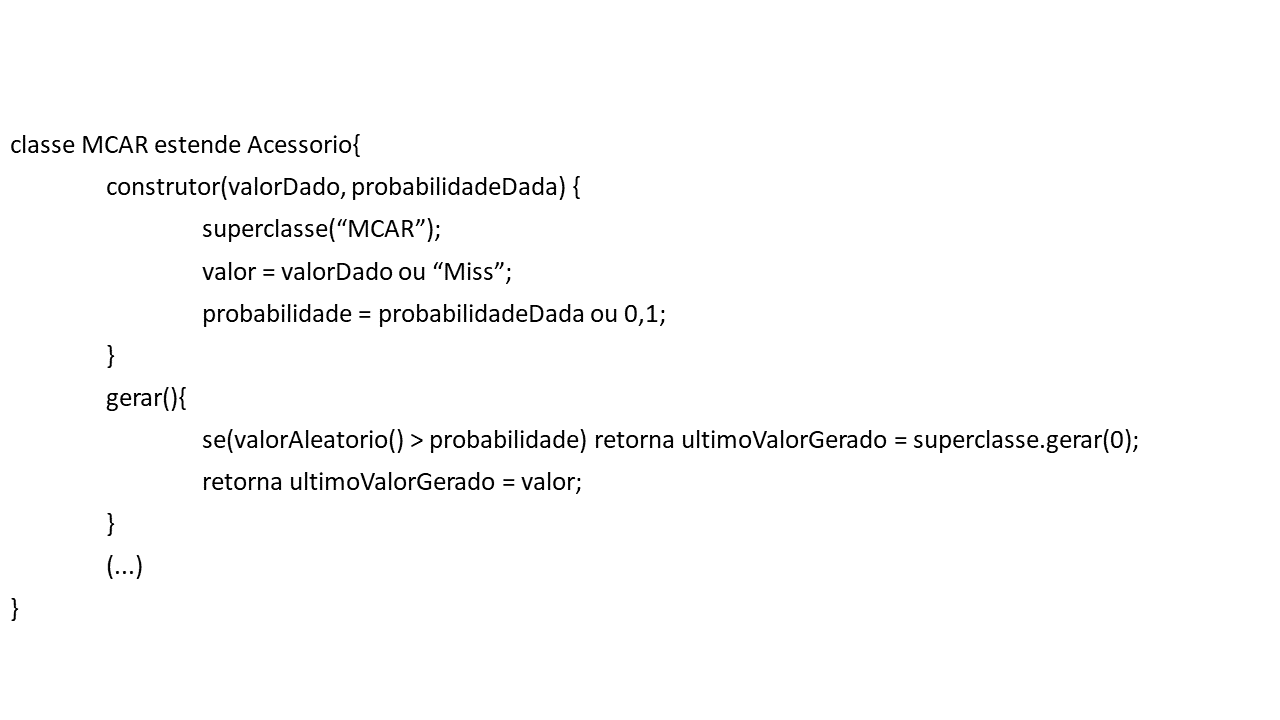
\includegraphics[width=\linewidth]{./figures/prototipo/MCAR.png}
			\label{fig:classeMCAR}
			\footnotesize Fonte: O autor do trabalho.
		\end{figure}
		\par
		%TODO: MNAR
		\pagebreak
		A classe do gerador MNAR (ver figura \ref{fig:MNARConstrutor}) foi dividida em 4 figuras, por conta do seu tamanho.
		Nesta figura, é possível ver os atributos no método construtor e 3 condições dentro do método gerar.
		O MNAR possui valor e probabilidade assim como o MCAR (figura \ref{fig:classeMCAR}), mas possui outros atributos para tratar os 3 tipos de dado.
		primeiroPadrao e segundoPadrao são úteis para o usuário colocar os valores de intervalo ou uma lista de categorias (somente para o primeiroPadrao).
		E a máscara é utilizada para determinar o formato do tempo utilizado e funciona somente para dados temporais.   
		\begin{figure}[h!]
			\centering
			\caption{Pseudocódigo sobre os atributos da classe MNAR do Blocks.}
			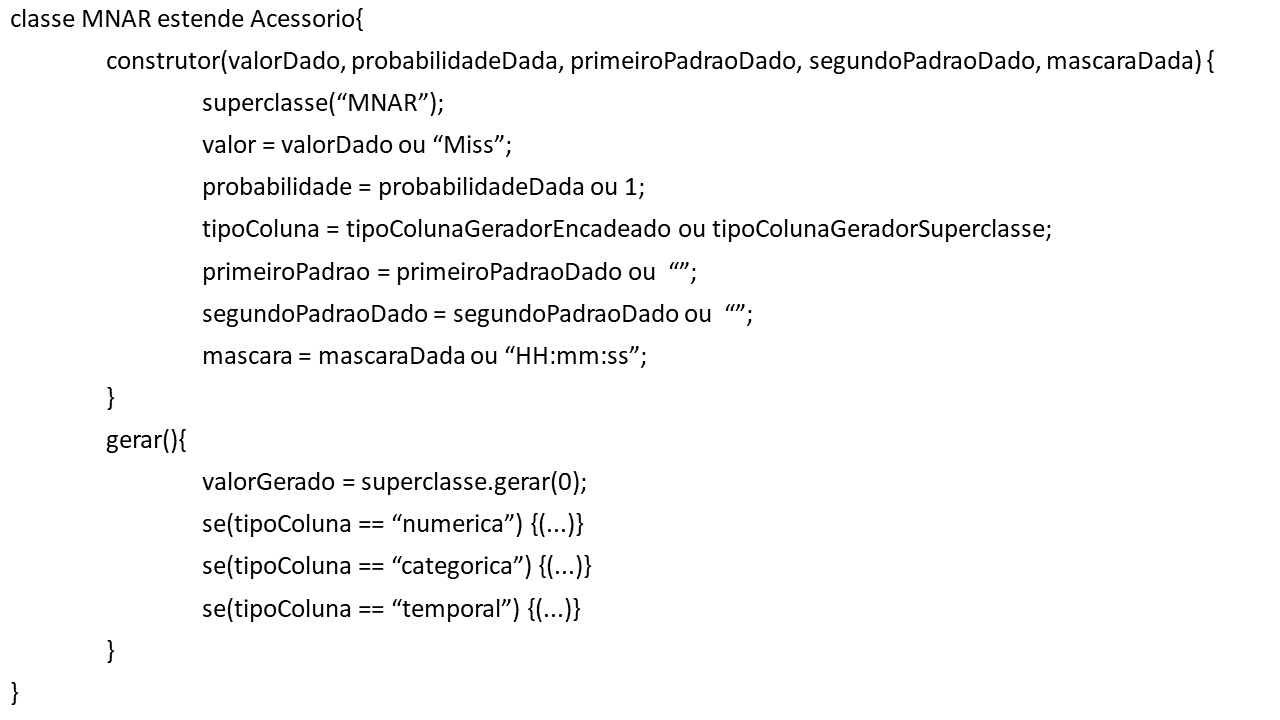
\includegraphics[width=\linewidth]{./figures/prototipo/MNARConstrutor.png}
			\label{fig:MNARConstrutor}
			\footnotesize Fonte: O autor do trabalho.
		\end{figure}
		\par
		Na figura \ref{fig:MNARNum} é apresentado como o gerador MNAR lida com dados numéricos.
		Primeiramente é verificado se a probabilidade é atendida, se não, é retornado o valor do gerador.
		Se sim, é verificado se o valor gerado (pelo gerador encadeado) entá no intervalo dado pelo usuário, se sim, o dado é faltante.
		\begin{figure}[h!]
			\centering
			\caption{Pseudocódigo sobre a classe MNAR do Blocks para dados numéricos.}
			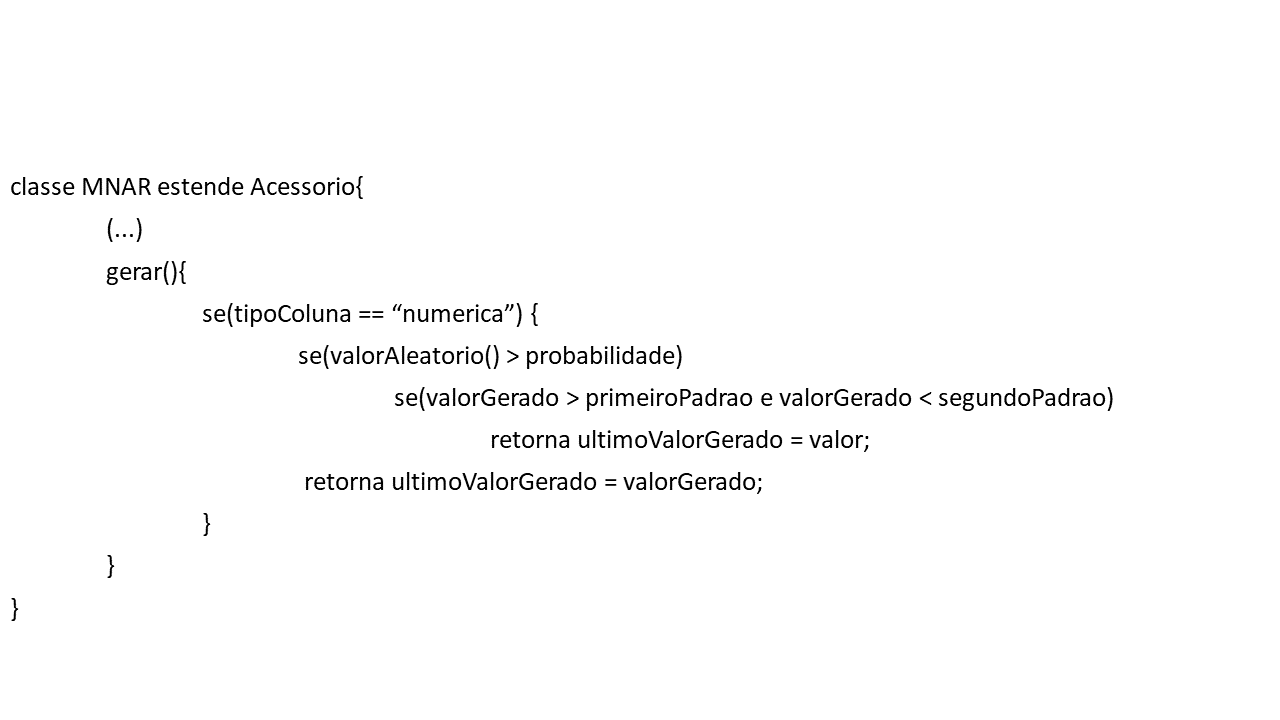
\includegraphics[width=\linewidth]{./figures/prototipo/MNARNum.png}
			\label{fig:MNARNum}
			\footnotesize Fonte: O autor do trabalho.
		\end{figure}
		Para dados categóricos (ver figura \ref{fig:MNARCat}) o gerador MNAR utiliza apenas o primeiroPadrao e, nesse caso, recebe uma lista de categorias.
		Depois de verificar a probabilidade, é verificado se a categoria gerada está na lista de categorias dada, se sim, o dado é faltante, se não é retornado o valor vindo do gerador encadeado.
		\begin{figure}[h!]
			\centering
			\caption{Pseudocódigo sobre a classe MNAR do Blocks para dados categóricos.}
			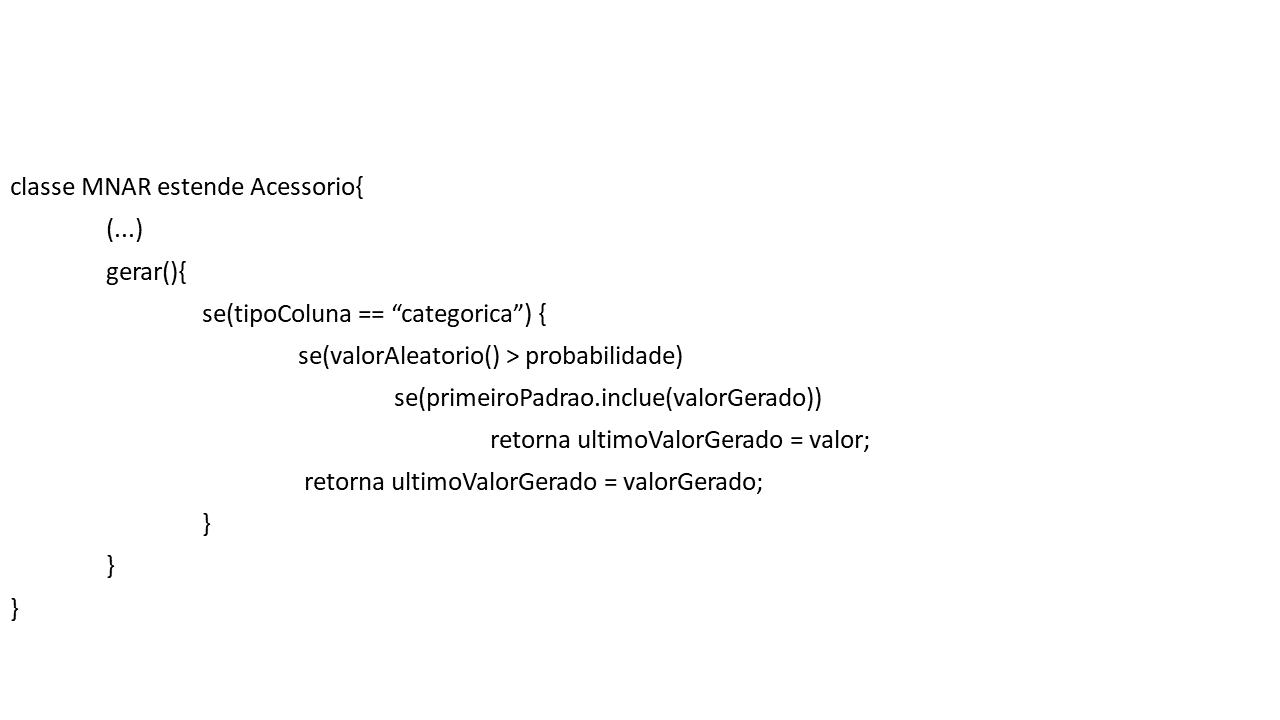
\includegraphics[width=\linewidth]{./figures/prototipo/MNARCat.png}
			\label{fig:MNARCat}
			\footnotesize Fonte: O autor do trabalho.
		\end{figure}
		O gerador MNAR para dados temporais (ver figura \ref{fig:MNARTemp}) funciona de forma similar para com dados numéricos \ref{fig:MNARNum}.
		Pois também utiliza do intervalo, no caso temporal, para determinar os dados faltantes.
		\begin{figure}[h!]
			\centering
			\caption{Pseudocódigo sobre a classe MNAR do Blocks para dados temporais.}
			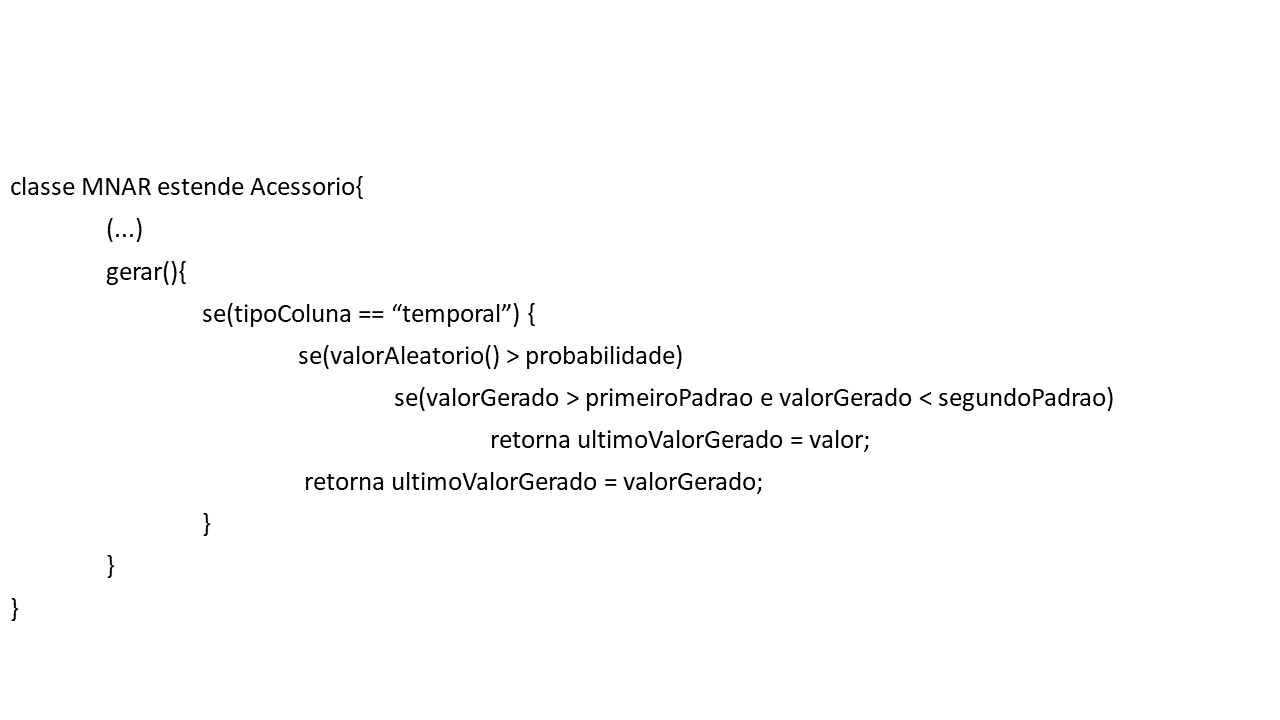
\includegraphics[width=\linewidth]{./figures/prototipo/MNARTemp.png}
			\label{fig:MNARTemp}
			\footnotesize Fonte: O autor do trabalho.
		\end{figure}
		%TODO: Noise
		O gerador \emph{Noise} (ver figura \ref{fig:classeNoise}) é um dos principais para geração de dados discrepantes.
		
		Ele utiliza também a probabilidade para ser a taxa de dados discrepantes e de um outro gerador para adicionar ruídos na dimensão.
		O nível de discrepância é dado pelo atributo intensidade, o qual multiplica o valor gerado.
		\begin{figure}[h!]
			\centering
			\caption{Pseudocódigo sobre a classe do Blocks.}
			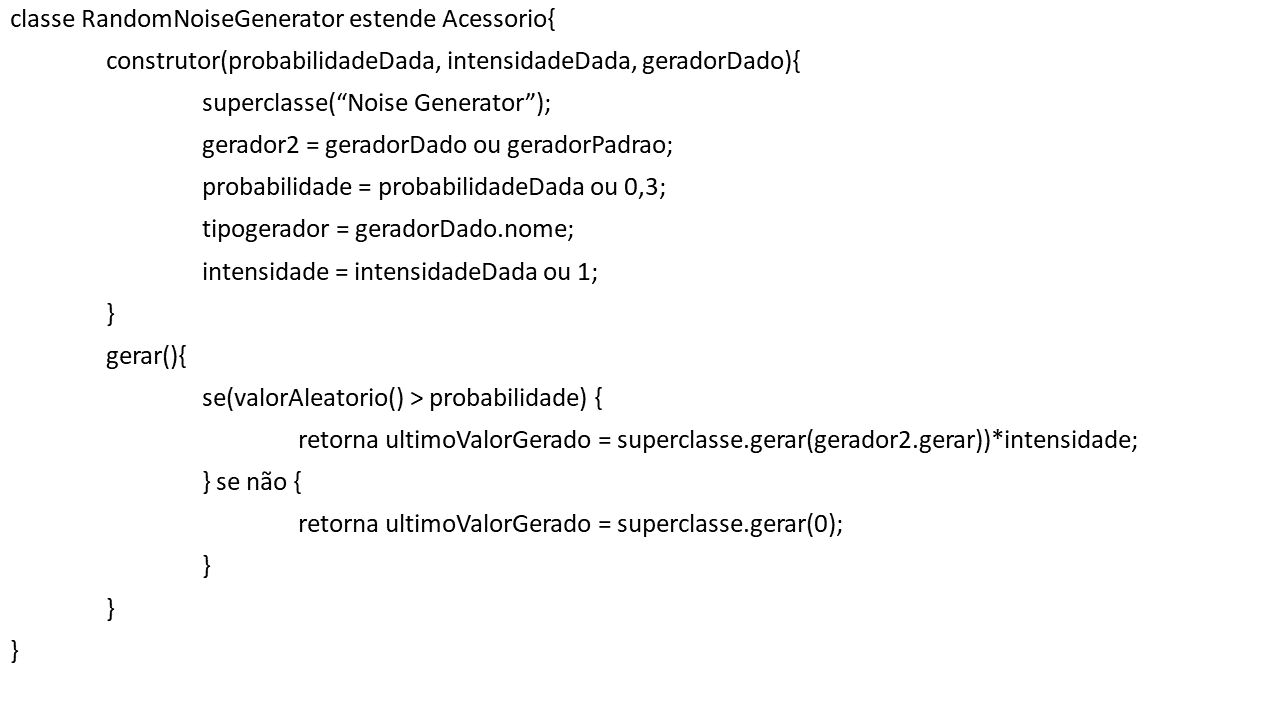
\includegraphics[width=\linewidth]{./figures/prototipo/Noise.png}
			\label{fig:classeNoise}
			\footnotesize Fonte: O autor do trabalho.
		\end{figure}
		\par
		%TODO: Constant Noise
		\pagebreak
		Já o gerador \emph{Constant Noise} (ver figura \ref{fig:classeConstantNoise}) funciona de forma semelhante ao \emph{Noise}, mas não possui o atributo intensidade.
		O seu método consiste em adicionar um ruído fixo em uma determinada amostra (definidade pela probabilidade) dos dados.

		\begin{figure}[h!]
			\centering
			\caption{Pseudocódigo sobre a classe do Blocks.}
			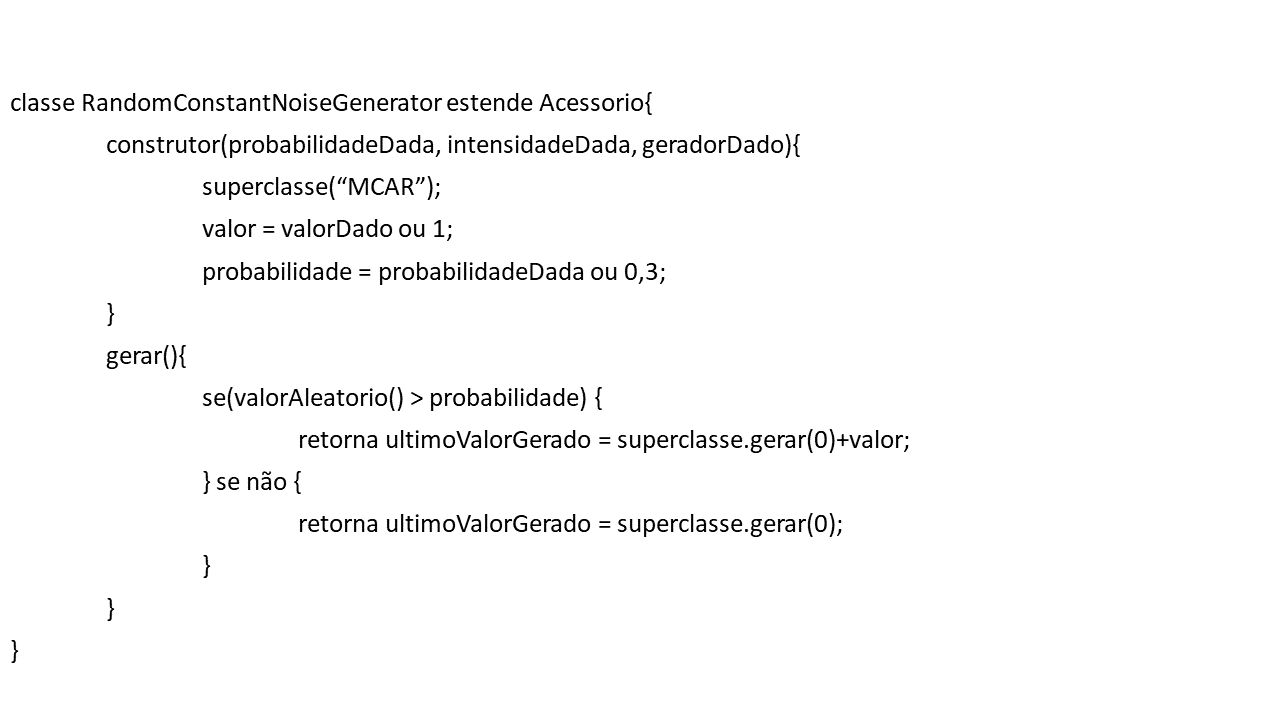
\includegraphics[width=\linewidth]{./figures/prototipo/ConstantNoise.png}
			\label{fig:classeConstantNoise}
			\footnotesize Fonte: O autor do trabalho.
		\end{figure}
% ---
\chapter{Sistema Blocks}
% ---
	Neste capítulo o sistema Blocks será apresentado em detalhes, como seu fluxo de funcionamento, funcionalidades, detalhes sobre a interface do usuário entre outros.
	De modo geral, o sistema é chamado de Blocks e visa ser um gerador de dados sintéticos baseado na combinação de modelos de dados.
	Assim, o usuário pode manipular um ou mais modelos e cada modelo pode conter N dimensões, que por sua vez podem conter M geradores de dados encadeados.
	\par
	Os geradores podem gerar dados numéricos, categóricos, temporais, entre outros. 
	O resultado de um gerador pode servir de entrada para outro através de operadores.
	Os operadores podem ou não aplicar uma operação matemática (soma, subtração, divisão ou multiplicação) ao resultado do gerador anterior - a leitura de anterior e posterior é da esquerda para a direita, respectivamente.
	Junto com os operadores, também há outras propriedades que variam de acordo com o gerador.
	\par
	Também é disponibilizado um pré-visualizador de dados com o gráfico coordenadas paralelas, o qual é colorido e interativo, sendo seu volume de dados independente do volume a ser gerado.
	Além do \emph{preview}, há uma integralização com um visualizador de dados mais elaborado e com mais opções de visualização, o \emph{VisApplication}.
	\par
	O Blocks permite gerar os dados em arquivos JSON, CSV, TSV ou por de requisições HTTP do tipo GET (\emph{Web Service}).
	Vale ressaltar que é possível configurar a quantidade de dados gerados, pré-visualizados, formato dos dados gerados, se contém o cabeçalho dos dados no arquivo final e as propriedades do \emph{Web Service}.
	\begin{figure}[h]
		\centering
		\caption{Fluxograma de utilização do Blocks.}
		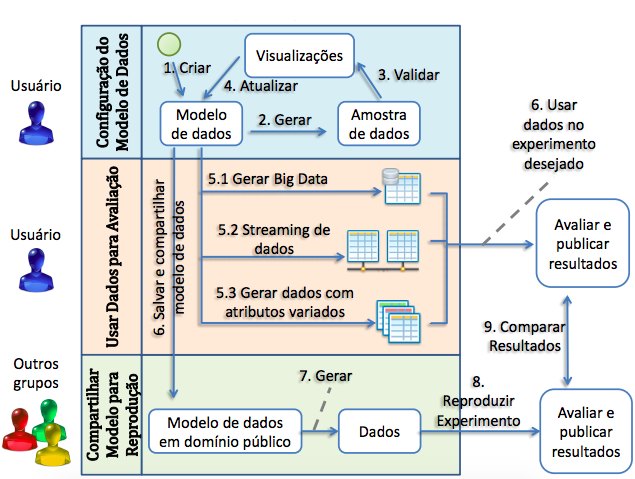
\includegraphics[width=\linewidth]{./figures/prototipo/fluxogramaUtilizacaoBlocks.png}
		\label{fig:fluxograma}
		\footnotesize Fonte: adaptado de (Brito Y., 2019).
	\end{figure}
	\par
	Na figura \ref{fig:fluxograma} é possível visualizar como foi pensada a utilização da aplicação.
	Na aba "Configuração do Modelo de Dados" encontra-se como o usuário pode configurar o modelo.
	O usuário define as dimensões e os seus geradores, assim como o comportamento dos dados pode ser validado pelo \emph{preview}. 
	Caso seja necessário, o modelo pode ser atualizado a qualquer momento.
	\par
	Na aba "Usar Dados para Avaliação" são demonstrados os caminhos para geração de dados.
	É possível a geração de dados por \emph{Big Data}, isto é, um grande conjunto de dados multidimensionais, apenas por meio de arquivos.
	Também é possível a geração de dados por \emph{Streaming}, a qual proporciona mais controle ao usuário sobre o processo de geração e também é disponibilizado o \emph{Web Service}.
	O caminho 5.3, visto na figura \ref{fig:fluxograma} demonstra uma forma iterativa de geração de arquivos de dados, com mudanças programadas de atributos.
	Esses dados podem ser usados em experimentos, testes e afins, cujos resultados podem ser publicados.
	\par
	E na aba "Compartilhar Modelo para Reprodução" é apresentado que os processos anteriores podem ser replicados a partir do mesmo modelo de dados e o resultado pode ser comparado, facilitando o consumo de dados por pesquisadores.
	
	\section{Tipos de Geradores de Dados}
		
		Na tabela \ref{table: Propriedade Geradores Blocks} são apresentados todos os geradores do Blocks até o momento desde trabalho.
		São apresentados seus nomes, suas categorias, o tipo de valores retornados, os tipos de parâmetros, se possui correlação - isto é, se é baseado no valor de outra dimensão - se são dependentes - ou seja, se precisa de um gerador encadeado para funcionar corretamente.
		
		\begin{table}[h]
			\centering
			\caption{Propriedade dos geradores do Blocks. 
				N=Numéro;
				C=Categoria;
				T=Tempo.
			}
			\vspace{0.5cm}
			\label{table: Propriedade Geradores Blocks}
			\begin{tabular}{c|c|c|c|c}
			
				Nome                 & Categoria  & T. dos valores                                            & Correlação & Dependente \\ % Note a separação de col. e a quebra de linhas
				\hline % para uma linha horizontal
				Constant             & Sequencial & N                                         & Não        & Não \\
				Counter              & Sequencial & N                                         & Não        & Não \\
				Fixed Time           & Sequencial & T                                         & Não        & Não \\
				Sinusoidal Sequence  & Sequencial & N                                         & Não        & Não \\
				Custom Sequence      & Sequencial & N                                         & Não        & Não \\
				%--------------------------------------------------------------------------------------------------------------------------------------------------------------------------------------------------------------------------------------------------------------------------
				Poisson Time         & Aleatório  & T                                         & Não        & Não \\
				Uniform              & Aleatório  & N                                         & Não        & Não \\
				Gaussian             & Aleatório  & N                                         & Não        & Não \\
				Poisson              & Aleatório  & N                                         & Não        & Não \\
				Bernoulli            & Aleatório  & N                                         & Não        & Não \\
				Cauchy               & Aleatório  & N                                         & Não        & Não \\
				Weighted Categorical & Aleatório  & C                                         & Não        & Não \\
				Categorical          & Aleatório  & C                                         & Não        & Não \\
				Categorical Quantity & Aleatório  & C                                         & Não        & Não \\
				%--------------------------------------------------------------------------------------------------------------------------------------------------------------------------------------------------------------------------------------------------------------------------
				Linear               & Função     & N                                         & Sim        & Não \\
				Quadratic            & Função     & N                                         & Sim        & Não \\
				Polynomial           & Função     & N                                         & Sim        & Não \\
				Exponential          & Função     & N                                         & Sim        & Não \\
				Logarithm            & Função     & N                                         & Sim        & Não \\
				Sinusoidal           & Função     & N                                         & Sim        & Não \\
				Categorical          & Função     & C                                         & Sim        & Não \\
				Piecewise            & Função     & N                                         & Sim        & Não \\
				TimeLaps             & Função     & T                                         & Sim        & Não \\
				%--------------------------------------------------------------------------------------------------------------------------------------------------------------------------------------------------------------------------------------------------------------------------
				MCAR                 & Acessório  & N, C ou T & Não        & Sim \\
				MNAR                 & Acessório  & N, C ou T & Não        & Sim \\
				Noise                & Acessório  & N, C ou T & Não        & Sim \\
				Constant Noise       & Acessório  & N, C ou T & Não        & Sim \\
				Range Filter         & Acessório  & N, C ou T & Não        & Sim \\
				Linear Scale         & Acessório  & N, C ou T & Não        & Sim \\
				No Repeat            & Acessório  & N, C ou T & Não        & Sim \\
				MinMax               & Acessório  & N, C ou T & Não        & Sim \\
				Low-Pass Filter      & Acessório  & N, C ou T & Não        & Sim \\
				Get Extra Value      & Acessório  & N, C ou T & Não        & Sim \\
				%--------------------------------------------------------------------------------------------------------------------------------------------------------------------------------------------------------------------------------------------------------------------------
				CubicBezier          & Geométrico & N                                         & Não        & Não \\
				Path2D Stroke        & Geométrico & N                                         & Não        & Não \\
				Path2D Fill          & Geométrico & N                                         & Não        & Não \\
			\end{tabular}
			\bigskip
			\\
			\footnotesize Fonte: O autor do trabalho.
		\end{table}

		

		% Na tabela \ref{table: Resumo Geradores Blocks} é apresentado um breve resumo para um entendimento abrangente do comportamento de cada gerador.

		% \begin{table}[h!]
		% 	\centering
		% 	\caption{Resumo dos geradores do Blocks}
		% 	% \vspace{0.5cm}
		% 	\label{table: Resumo Geradores Blocks}
		% 	\begin{tabular}{l|p{13.3cm}}
			
		% 		Nome                 & Resumo \\ % Note a separação de col. e a quebra de linhas
		% 		\hline % para uma linha horizontal
		% 		Constant             & Sequência de \textbf{números} com sempre o mesmo número.\\
		% 		Counter              & Sequência de \textbf{números} que é incrementada ou decrementada.\\
		% 		Fixed Time           & Sequência de \textbf{tempo} que é incrementada ou decrementada.\\
		% 		Sinusoidal Sequence  & Sequência de \textbf{números} de acordo com uma função senoidal.\\
		% 		Custom Sequence      & Sequência de \textbf{números} cujo comportamento é dado pelo usuário.\\
		% 		%--------------------------------------------------------------------------------------------------------------------------------------------------------------------------------------------------------------------------------------------------------------------------
		% 		Poisson Time         & Valores aleatórios \textbf{temporais} em uma distribuição de de Poisson.\\
		% 		Uniform              & Valores aleatórios \textbf{númericos} em uma distribuição uniforme.\\
		% 		Gaussian             & Valores aleatórios \textbf{númericos} em uma distribuição Normal.\\
		% 		Poisson              & Valores aleatórios \textbf{númericos} em uma distribuição de de Poisson.\\
		% 		Bernoulli            & Valores aleatórios \textbf{númericos} em uma distribuição de de Bernoulli.\\
		% 		Cauchy               & Valores aleatórios \textbf{númericos} em uma distribuição de de Cauchy.\\
		% 		Weighted Categorical & Valores aleatórios \textbf{categóricos} dadas as categorias com probabilidade ponderada.\\
		% 		Categorical          & Valores aleatórios \textbf{categóricos} dadas as categorias.\\
		% 		Categorical Quantity & Valores aleatórios \textbf{categóricos} dadas as categorias definindo a quantidade de aparição de categorias. \\
		% 		%--------------------------------------------------------------------------------------------------------------------------------------------------------------------------------------------------------------------------------------------------------------------------
		% 		Linear               & Valores a partir de uma dimensão \textbf{númerica} em uma função linear.\\
		% 		Quadratic            & Valores a partir de uma dimensão \textbf{númerica} em uma função quadrática.\\
		% 		Polynomial           & Valores a partir de uma dimensão \textbf{númerica} em uma função polinomial.\\
		% 		Exponential          & Valores a partir de uma dimensão \textbf{númerica} em uma função exponencial.\\
		% 		Logarithm            & Valores a partir de uma dimensão \textbf{númerica} em uma função logarítmica.\\
		% 		Sinusoidal           & Valores a partir de uma dimensão \textbf{númerica} em uma função senoidal.\\
		% 		Categorical          & Valores a partir de uma dimensão \textbf{categórica}.\\
		% 		Piecewise            & Valores a partir de uma dimensão \textbf{númerica} com limiar para 2 encadeamentos. \\
		% 		TimeLaps             & Valores a partir de uma dimensão \textbf{temporal} que gera dados ao atingir um tempo.  \\
		% 		%--------------------------------------------------------------------------------------------------------------------------------------------------------------------------------------------------------------------------------------------------------------------------
		% 		MCAR                 & Valores faltantes aleatoriamente um ou mais geradores dada uma probabilidade. \\
		% 		MNAR                 & Valores faltantes aleatoriamente um ou mais geradores dada uma lógica. \\
		% 		Noise                & Valores ruidosos um mais geradores dada uma probabilidade e intensidade. \\
		% 		Constant Noise       & Dados ruidosos com valor constante um mais geradores dada uma probabilidade. \\
		% 		Range Filter         & Dado um ou mais geradores, os dados que estão no intervalo não são gerados.\\
		% 		Linear Scale         & Dado um ou mais geradores, os dados são escalados de acordo com os parâmetros definidos. \\
		% 		No Repeat            & Dado um ou mais geradores, são retirados os dados repetidos. \\
		% 		MinMax               & Permite escolher qual será o valor máximo e o mínimo gerados. \\
		% 		Low-Pass Filter      & Dado um ou mais geradores, este simula o resultado de um filtro passa-baixa.\\
		% 		Get Extra Value      & Recebe o valor de dados multidimensionais. \\
		% 		%--------------------------------------------------------------------------------------------------------------------------------------------------------------------------------------------------------------------------------------------------------------------------
		% 		CubicBezier          & Dados para desenhar uma curva Bezier cúbica. \\
		% 		Path2D Stroke        & Dados para desenhar a borda de um polígono. \\
		% 		Path2D Fill          & Dados para preencher um polígono. \\
		% 	\end{tabular}
		% 	\bigskip
		% 	\\
		% 	\footnotesize Fonte: O autor do trabalho.
		% \end{table}

		\subsection{Sequencial}
			Os geradores da categoria Sequencial geram valores encadeados dado um padrão.
			É possível gerar o próprio padrão a partir do gerador \emph{Custom Sequence}, o qual você determina um valor Inicial (\emph{Begin}) e o valor Intervalar (\emph{Step}), isto é, o qual vai ser incrementado ou decrementado dado uma Sentença (\emph{sentence}) customizada.
			\par
			Contudo, já são predefinidos alguns geradores como 
				o \emph{Constant}, o qual define um valor único de geração;
				o \emph{Counter}, funciona como um contador, no qual é definido o valor Inicial e o Intervalar;
				o \emph{Fixed Time Generator} gera um intevalo de tempo, no qual pode ser definido o valor inicial (\emph{init}), Intervalar e a máscara (\emph{mask}), isto é, como o tempo deve ser formatado;
				o \emph{Sinusoidal Sequence} gera de acordo com a função senoidal, que, além do valor Inicial e Intervalar, há o 'a' de Amplitude, 'b' de frequência ângular e 'c' para representar a fase da onda.

		\subsection{Aleatório}
			A categoria aleatória de dados contém um grande número de geradores, pois existe uma diversidade de distribuições de probabilidade comparada às outras categorias.
			\par
			Esta categoria conta com geradores uniformes, isto é, a distribuição dos dados é equalizada;
				Também há um gerador de dados de tempo, parecido com o \emph{Fixed Time Generator} com a diferença que o comportamento é definido pela fórmula de \emph{Poisson} e que há mais duas configurações: unidade de tempo - a qual pode ser desde milissegundos a anos - e o lambda, advindo da fórmula.
				Há uma distribuição de \emph{poisson} também, apenas com o lambda;
				É disponibilizado geradores de fórmulas clássicas com a normal (\emph{Gaussian}), \emph{Bernoulli}, e \emph{Cauchy} com seus devidos parâmetros.
			\par
			Além de números, também é possível gerar dados categóricos (\emph{Categorical}), dadas as palavras - também chamado de categorias - inicialmente.
				Similarmente há o \emph{Weighted Categorical} que possui valores de probabilidade para cada palavra, e 
				já o \emph{Categorical Quantity}, em vez de probabilidade, define quantas vezes cada palavra deve aparecer.
		\subsection{Função}
			A categoria funções (\emph{Function}) serve para gerar dados de acordo com outra dimensão chamado de \emph{input}, isto é, facilita a correlação entre dimensões.
			Para dados numéricos, disponibiliza-se as 
				função de primeiro grau (\emph{Linear Function}), 
				segundo grau (\emph{Quadratic Function}), 
				exponencial (\emph{Exponential Function}), 
				logarítmica (\emph{Logarithm Function}) e
				a \emph{Piecewise Function}, cuja função é definida por subfunções, e no caso, é possível definir o gerador desejado até um determinado valor chamado de \emph{Intervals} e depois pode-se escolher outro gerador.
			\par
			Para dados categóricos, há a função categórica (\emph{Categorical Function}) e 
			a \emph{TimeLaps Function} a qual funciona de forma semelhante ao gerador \emph{Piecewise Function}, só que utiliza uma quantidade de tempo como limiar - imagine uma corrida de fórmula 1 e cada vez que os carros passam pela linha de chegada eles completam uma volta. 
			Esta volta é o limiar também chamado de \emph{Laps} - e para o \emph{input}, somente geradores de tempo.
		\subsection{Acessório}
			Os geradores da categoria Acessórios (\emph{Acessory}) foram pensados especialmente para serem concatenados com outros geradores, com o fim de incrementá-los.
			Entre os geradores acessórios, pode-se citar o \emph{Missing Value}, o qual foi subdivido em 2 geradores: o \emph{MCAR} e \emph{MNAR}.
			\par
			O MCAR usa a probabilidade para definir se um dado será faltante;
			O MNAR trabalha de forma diferente para cada tipo de dado.
			Os tipos de dado são os Numéricos, os Categóricos e os Temporais.
			\par
			O MAR é gerado a partir do encadeamento de geradores.
			Isto é, por conta do MAR levar em consideração a correlação a uma dimensão,
			este pode utilizar um gerador da categoria função em conjunto do MCAR ou MNAR.
			\par
			Para os Numéricos e os Temporais, é definido um intervalo no qual os dados vão ser faltantes.
			Para os dados Categóricos, é definida uma lista de categorias na qual todas essas categorias faltarão na geração de dados.
			\par
			 Os geradores MNAR e o MCAR foram desenvolvidos ou modificados no sistema ao longo deste trabalho.
			 Entretanto a implementação foi baseada nos artigos \cite{twala2009empirical} \cite{xia2017adjusted} para implementação do MNAR,
			 os trabalhos de \cite{rieger2010random} \cite{xia2017adjusted} são semelhantes ao gerador MCAR, pois utilizam uma probabilidade para definir aleatoriamente um dado faltante.
			 Os artigos de implementação também podem ser encontrados no artigo \cite{santos2019generating} e segundo o mesmo, as implementações são consideradas univariadas, isto é, apenas uma dimensão é afetada.
			  
			\par
				O \emph{Noise Generator} que adiciona dados fora do padrão, conhecido como ruído, com uma determinada probabilidade, intensidade - o que ajuda a criar o nível de discrepância - e a partir de três distribuições: uniforme, normal e de Poisson.
				O \emph{Constant Noise Generator} também adiciona ruídos, mas só que é um valor específico com determinada probabilidade de ser adicionado;
				o \emph{Ranger Filter} permite retirar do conjunto de dados os valores que estão entre os valores de início (\emph{Begin}) e fim (\emph{End});
				o \emph{Linear Scale} permite que os determinados (selecionados através do \emph{MinIn} e \emph{MaxIn}) dados sejam escalados através do \emph{minOut} e \emph{MaxOut}.
			\par
			O \emph{No Repeat} retira dados repetidos do conjunto;
				o \emph{MinMax} define quais valores serão os maiores e menores de acordo com os parâmetros dados;
				o \emph{Low-Pass Filter} realiza um filtro passa-baixa nos dados. Ou seja, o valor sucessor é uma media ponderada (valor recebido pelo parâmetro \emph{Smooth}) do valor anterior com o valor gerado;
				o \emph{Get Extra Value} pega os retornos extras dos geradores que retornam mais que um valor.
		\subsection{Geométrico}
			Os geradores Geométricos (\emph{Geometric}) permitem que seja gerado dados a partir de formas geométricas.
			Para isso são disponibilizados três geradores.
			O primeiro deles (\emph{Path2D Stroke}) gera dados bidimensionais presentes nas arestas de um polígono inserido pelo usuário.
			O segundo (\emph{Path2D Fill}) gera os dados pertencentes do polígono inserido pelo usuário.
			Quanto ao terceiro (\emph{CubicBezier}), este gera dados para desenho de uma curva bezier cúbica a partir de seus pontos.
		\subsection{Baseado em dados reais}
			Para esta categoria, existe um gerador, chamado como \emph{Real Data Wrapper}.
			Ele é criado automaticamente quando o usuário importa um conjunto de dados reais através de um CSV.
			Este gerador recebe tantos valores categóricos como numéricos e essa informação pode ser decidida automaticamente pelo gerador ou ser forçada pelo usuário.
			É possível gerar uma quantidade superior de dados em relação ao conjunto de dados real, para isso é feito um tratamento de inputação de dados.
			Esse tratamento é feito por meio de funções de geração, chamadas de \emph{GenType}.
			\par
			Essas funções podem ser do tipo \emph{Standart}, que utiliza os dados do início ao fim de forma cíclica até chegar ao número desejado de registros.
			Também pode ser do tipo \emph{Reverse} que ao contrário do \emph{Standart}, utiliza os dados do final ao início.
			É disponibilizado o modo aleatório (\emph{Random}) e outras variações.
			\par
			A primeira variação do modo aleatório é o \emph{QuartileRandom}, que divide o conjunto de dados em três marcos e a probabilidade de se pegar um dado daquele quartil é proporcional ao tamanho do marco.
			A leitura dos Marcos pode ser visualizada na figura \ref{fig:leituraMarco}. Então, se o valor do espaço entre 0 e quartil 1 for 100, todos os dados gerados serão do primeiro 1/4 do conjunto de dados.
			A segunda variação é o \emph{AverageRandom} que utiliza o valor da média e da variancia - [Média - Variancia, Média + Variancia] de um conjunto de dados númerico ou utiliza os N valores categóricos mais frequentes com distribuição uniforme.
			\begin{figure}[h]
				\centering
				\caption{Ilustrando a leitura dos marcos dos quartis. O tamanho do espaço entre os quartis ou entre 0 ou o 100 é o valor da probabilidade de um número ser desse espaço.}
				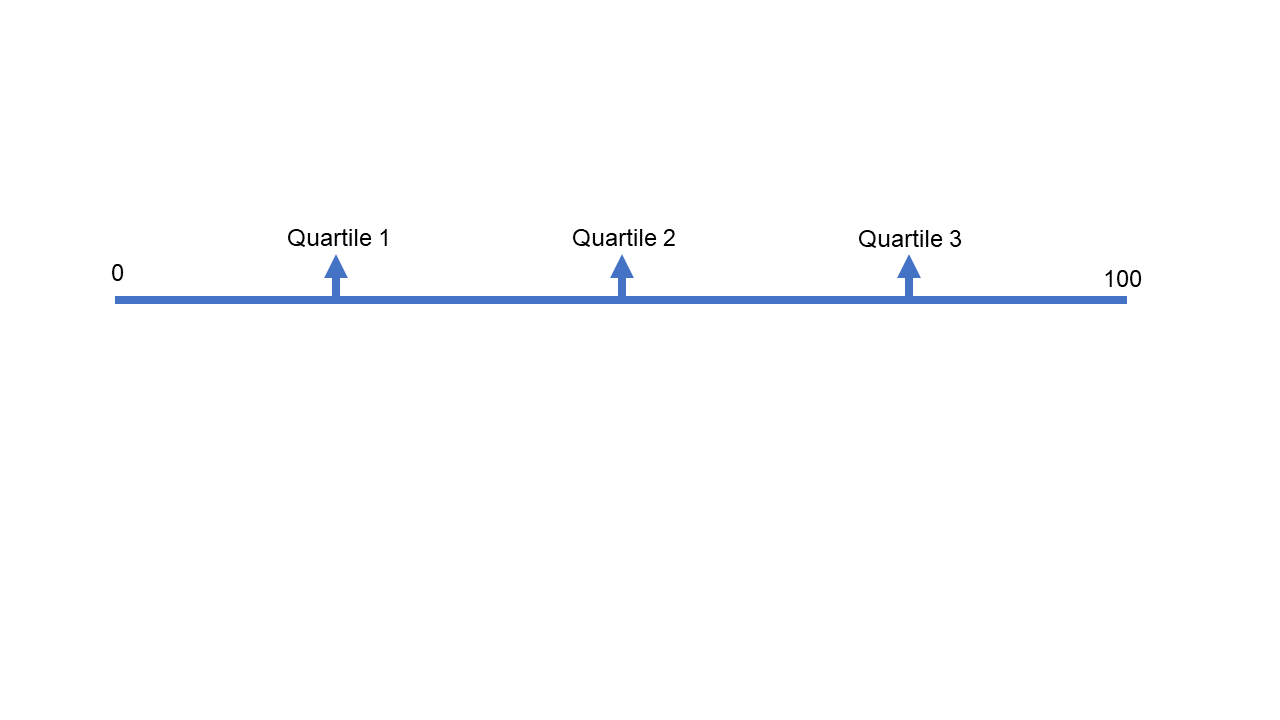
\includegraphics[width=\linewidth]{./figures/prototipo/quartil.png}
				\label{fig:leituraMarco}
				\footnotesize Fonte: O autor do trabalho.
			\end{figure}
	\section{Modos de Geração de Dados}
		Nessa seção é demonstrado como é feita a concretização do comportamento dos geradores, isto é, os dados propriamente ditos.
		Gerar os dados é tão importante quanto gerar o modelo, visto que os dados gerados podem ser utilizados para testes de aplicações, por exemplo.
		\par
		Os dados são gerados por \emph{Web Service} e em dois tipos de memória: a primária e a secundária.
		A memória primária serve de base para escrever na memória secundária e também alimenta as visualizações de dados.
		\subsection{\emph{Streaming Data}}
			Para otimizar a geração de grande volumes de dados, foi utilizado o conceito de \emph{Streaming Data}, isto é, gerar o volume de dados aos poucos - em blocos - para que não haja estouro de memória primária.
			Também foi utilizado esse processo assincronamente, para que a interface de usuário não seja bloqueada durante o processo e permitir que o progresso da geração seja acompanhado.
			\par
			O usuário escolhe a quantidade de dados a ser gerada e a aplicação define automaticamente a quantidade de blocos.
			Cada bloco é fixado em até 10.000 instâncias.
			Esse valor foi definido de forma aleatória.
			Mais testes serão feitos com o intuito otimizar o número de instâncias de cada bloco.
			O bloco é processado e armazenado temporariamente na memória primária até que ele esteja completo.
			Então, o bloco é escrito na memória secundária.
		\subsection{Web Service}
			Quanto ao \emph{Web Service}, este foi pensado para facilitar o teste de aplicação.
			Cada modelo é independente, isto é, podem ser habilitados somente os modelos desejados para distribuição.
			E além da configuração por dentro do \emph{software}, também é possível criar configurações temporárias para cada requisição, sem alterar as configurações do modelo.
			\par
			Os parâmetros disponíveis para configuração temporária pela URI são: o nome do modelo, o formato dos dados e a quantidade de registro.
			É disponibilizado um ícone de aviso ao usuário quando um modelo está distribuindo dados via \emph{Web Service} na aba do modelo.
			Um exemplo de URI para fazer requisição HTTP do tipo GET é: (\url{http://localhost:8000/?modelid=MODEL_r6w2ffk3.mva&nsample=100&format=csv}), nos quais "modelid" é o \emph{ID} do modelo, "nsample" é a quantidade de instâncias desejada e "format" é o formato do arquivo desejado.
	 
	\section{Modos para Visualização de Dados}
		O sistema permite modelar os dados, gerá-los e também visualizá-los.
		Nessa seção são mostradas as duas formas de visualizar dados no Blocks.
		A primeira fica acessível na tela inicial do gerador chamado de \emph{Preview}.
		A outra é um programa a parte que é integrado ao Blocks, isto é, há o compartilhamento do modelo de dados.

		\subsection{Preview}
			O pré-visualizador de dados foi criado pensando em oferecer uma visualização rápida e abrangente do modelo de dados.
			Para isso, foi escolhido o gráfico Coordenadas Paralelas, por conta de sua característica de visualização prática de dados multidimensionais.
			Também foram adicionadas algumas características extras como diferenciação por cores (mapa de calor para dados numéricos e cor única para dados categóricos); 
				filtro de dimensão, para que fosse visualizado apenas o que for necessário;
				escolha de dimensão como referencial, isto é, a partir da dimensão escolhida, verificar como os dados se comportam nas outras dimensões. Isso pode ser ativado tanto clicando sobre o nome da dimensão, quanto através do \emph{ComboBox} acima do \emph{preview};
				também é possível recarregá-lo e desativá-lo, para travamentos quando for trabalhar com \emph{Big Data}, por exemplo.

		\subsection{Módulo de Visualização Externo e Integrado}
			O módulo chamado VisApplication é um conjunto de técnicas de visualização reutilizáveis.
			Ela pode chamada por dentro do Blocks e já pode utilizar os dados do modelo atual.
			Dentre as visualizações disponíveis pode-se citar as Coordenadas Paralelas, \emph{Scatter Plot}, \emph{Treemap}, \emph{Sunburst}, \emph{Bar Chart} entre outros.
			Como diferencial, algumas funcionalidades são adicionadas como detalhe sob demanda, \emph{zoom}, marcação de dados (\emph{Highlight}), múltiplas visualizações simultâneas, entre outras.
	
	\section{Estrutura da Interface Gráfica do Blocks}
		O sistema possui uma interface gráfica para \emph{Desktop} e segue um modelo de estrutura que possui uma janela principal, mais algumas janelas auxiliares.
		Isso significa que há uma tela com as principais informações (ver figura \ref{fig:telaPrincipal}), e outras informações mais específicas são visualizadas através de \emph{tabs}, \emph{modals}, \emph{alerts} e correlacionados.
		\begin{figure}[h]
			\centering
			\caption{Conhecendo os elementos da tela principal do Blocks, na sua versão para Windows.}
			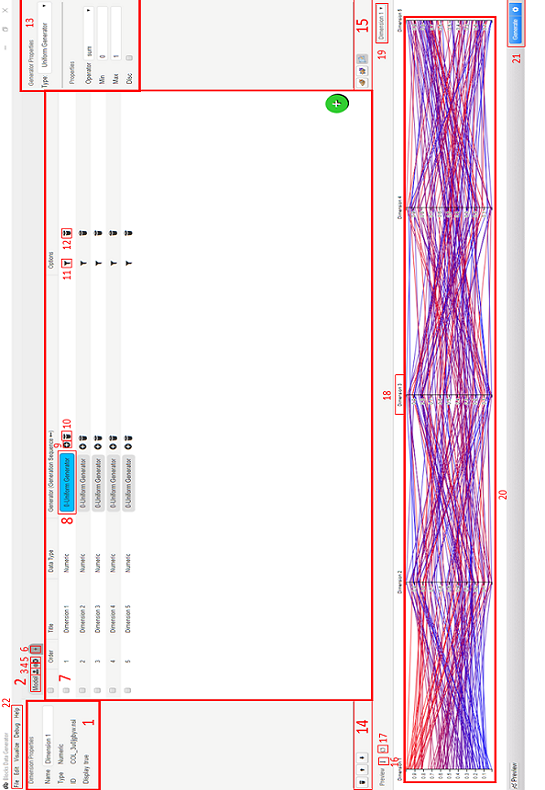
\includegraphics[width=\linewidth]{./figures/prototipo/telaprincipalmarcada.png}
			\label{fig:telaPrincipal}
			\footnotesize Fonte: O autor do trabalho.
		\end{figure}
		\begin{figure}[h]
			\centering
			\caption{Conhecendo os elementos da tela de configurações para geração de dados.}
			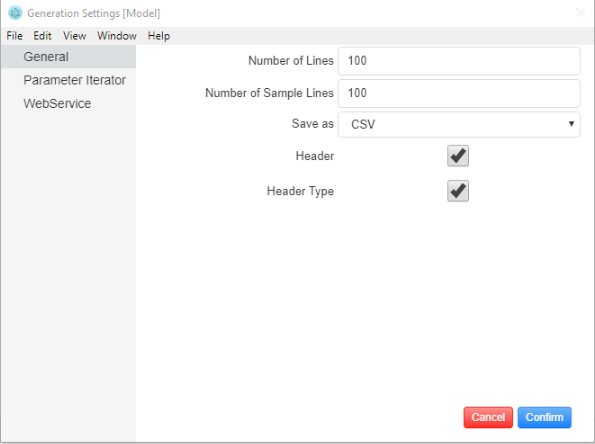
\includegraphics[width=\linewidth]{./figures/prototipo/generationSettings.png}
			\label{fig:generationSettings}
			\footnotesize Fonte: O autor do trabalho.
		\end{figure}
		\par
		Na figura \ref{fig:telaPrincipal} pode-se encontrar os principais elementos para utilizar o Blocks.
		Nesta digura são encontradas 22 marcações e serão descritas na lista a seguir.
		\begin{enumerate}
			\item São definidas as propriedades da dimensão, é possível visualizar informações e alterar o título;
			\item Nome atual do modelo;
			\item Ícone para mostrar que este modelo está servindo dados via (\emph{Web Service});
			\item Ícone para mostrar alterações não salvas no modelo;
			\item Botão para fechar o modelo;
			\item Espaço para as dimensões do modelo;
			\item Botão para criar um novo modelo;
			\item Gerador;
			\item Botão responsável por criar e aumentar o encadeamento de geradores;
			\item Botão para excluir um gerador da cadeia;
			\item filtro de dimensões - quando este ícone estiver com uma reta na diagonal sobre o filtro, significa que a dimensão não será incluída na geração e nem visualização dos dados;
			\item Botão para excluir a dimensão selecionada;
			\item Configurações atuais do gerador - tipo de gerador, que apresenta uma lista de categorias que, por sua vez, cada uma apresenta uma lista de geradores e também as propriedades do gerador selecionado;
			\item Botões para excluir ou alterar o posicionamento da dimensão selecionada;
			\item Botões para copiar geradores;
			\item Botão para esconder o pré-visualizador de dados;
			\item Botão para recarregar o pré-visualizador de dados;
			\item Ao clicar no título, a dimensão é selecionada como origem para as cores;
			\item \emph{ComboBox} para selecionar dimensão para dar origem às cores - útil para saber como os dados da dimensão selecionada se comporta nas outras dimensões.
			\item Pré-visualizador de dados utilizando o Coordenadas Paralelas;
			\item Botões para gerar os dados a partir do modelo atual e para manipular as algumas configurações do modelo atual;
			\item Agrupa botões para abrir, criar, ou salvar um modelo; desfazer ou refazer uma alteração ou abrir o \emph{VisApplication}.
		\end{enumerate}
		\par
		Ao clicar com o botão direito do \emph{mouse} no título do modelo (M2) aparece um menu, como visto na figura \ref{fig:contextMenu}.
		Esse \emph{context menu} permite renomear ou deletar o modelo, exportá-lo como arquivo .DOT e também manipular algumas informações para o Web Service Como
			copiar para a área de transferência o ID do modelo, uma URI padrão (\emph{localhost}); ativar ou desativar o modelo pra \emph{Web Service}, bem como abrir a URI em um software padrão do usuário.
		\begin{figure}[h]
			\centering
			\caption{Conhecendo os elementos da \emph{context menu} na aba do modelo.}
			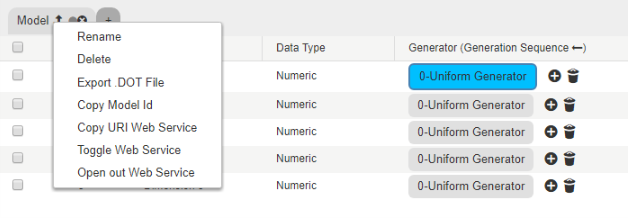
\includegraphics[width=\linewidth]{./figures/prototipo/contextMenu.png}
			\label{fig:contextMenu}
			\footnotesize Fonte: O autor do trabalho.
		\end{figure}
		\par
		Ao lado do botão (\emph{Generate}) para iniciar a geração é encontrado outro botão com o ícone de engrenagem (M21).
		Na figura \ref{fig:generationSettings}, no lado esquerdo, encontra-se 3 seções.
		A primeira é dedicada para configurações gerais do modelo, como quantidade de dados para ser gerados, mostrado no \emph{preview} ou formato dos dados.
		A segunda seção (\emph{Parameter Iterator}) foi desenvolvida para quem precisar criar mais de um arquivo variando apenas alguns parâmetros, de forma iterativa.
		A terceira seção é especial para o \emph{Web Service} no qual, liga ou desliga o servidor ou troca a porta padrão para servir os dados.
		
		\subsection{Mensagens para o usuário}
			O sistema precisa avisar o usuário de falhas, perguntar sobre preferências e afins.
			Para isso, o Blocks utiliza-se de \emph{Dialogs} para receber um caminho para salvar ou abrir um arquivo.
			Há um espaço dedicado na tela principal para mensagens advindas de um processo de geração de dados.
			Mensagem para preparação, progresso, finalização ou falha na geração de dados pode ser acompanhado pelo \emph{Footer Display}. (ver figura \ref{fig:SDvisor}).
			Para outros avisos mais genéricos como erros ou tarefas bem sucedidas, bem como avisos mais detalhados há o \emph{Modal}.
			Também há Atalhos do Teclado da aplicação Blocks para demonstrar os atalhos do teclado, para melhorar a eficiência de usuários que preferem esse recurso.
			\begin{figure}[h]
				\centering
				\caption{Conhecendo o \emph{Footer Display} na tela Inicial do Blocks.}
				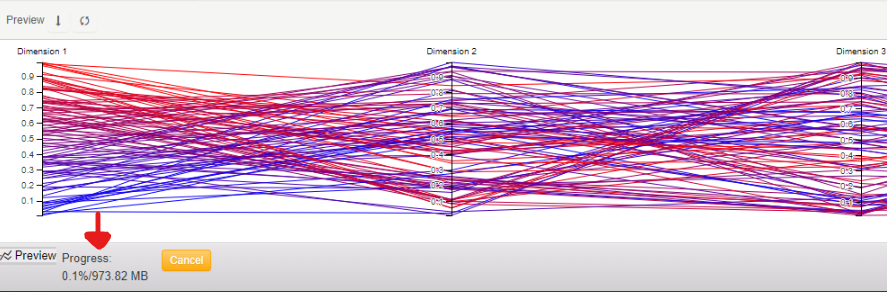
\includegraphics[width=\linewidth]{./figures/prototipo/SDvisor.png}
				\label{fig:SDvisor}
				\footnotesize Fonte: O autor do trabalho.
			\end{figure}

% ---
\chapter{Validação Visual}
	Este capítulo é dedicado a apresentar como podem ser modelados os dados discrepantes e faltantes no Blocks.
	Também, serão apresentados os dados gerados e técnicas de visualização a partir das possibilidades do sistema.
	\par
	
	\section{Modelagem dos Dados}

		Foram criadas cinco bases de dados de contextos genéricos, simulando abstratamente contextos reais.
		Para criação dessas bases com 500 instâncias foram utilizados os geradores
		 \emph{Noise Generator} e o \emph{Constant Noise Generator} para gerar dados discrepantes.
		E para criação de dados faltantes foram utilizados os geradores
		 \emph{MCAR}, \emph{MAR} e \emph{MNAR}.
		Também foram utilizados outros geradores para auxiliar no comportamento das dimensões como os
		 \emph{Linear Funcion}, \emph{Linear Scale}, \emph{MinMax} e 
		 \emph{Piecewise Function}.
		\par

		A primeira base é sobre uma avaliação de carros, onde há os seguintes atributos: 
		categoria do carro,
		ano,
		marca,
		preço,
		notas dos críticos e do público.
		Como pode ser visto na figura \ref{fig:CarrosModelo}, Categoria e Marca são um conjunto de palavras genéricas e uniformente distribuídas, assim como o Ano do carro, mas com números inteiros.
		\par
		O preço já tem um tratamento de discrepância - os carros podem ficar 30\% mais caros ou mais baratos - e uma correlação com o ano - pois carros mais velhos tendem a ficar mais baratos.
		A nota dos críticos é gerada de forma uniforme e imparcial, para ser um referencial técnico.
		\par
		Contudo, houve uma configuração de MNAR na modelagem, na qual as notas abaixo de 2 estão faltando, propositalmente.
		A nota do público tem dados faltantes com relação ao simples fato de uma pessoa preferir não opinar sobre o assunto e correlação com o preço - inversamente proporcional - e nota dos críticos - diretamente proporcional.
		Quando a nota dos críticos é faltante, o público leva em consideração apenas o preço.
		\par
		\begin{figure}[h!]
			\centering
			\caption{Base sintética de avaliação de Carros.}
			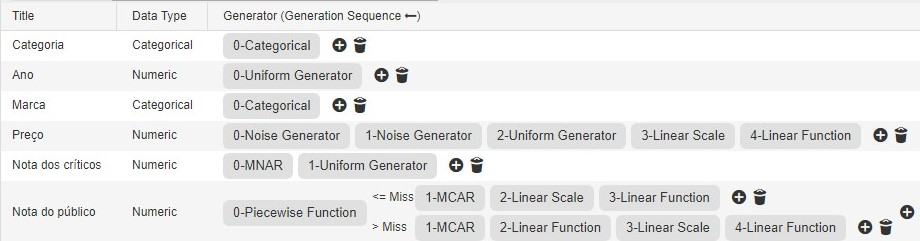
\includegraphics[width=\linewidth]{./figures/Resultados/CarrosModelo.jpg}
			\label{fig:CarrosModelo}
			\footnotesize Fonte: O autor do trabalho.
		\end{figure}

		A segunda base (ver figura \ref{fig:RSmodelo}) diz respeito a uma avaliação de Redes Sociais.
		As dimensões presentes são
		 o nome que é uma categoria genérica;
		 idade que varia de 18 a 65 anos - mas possui dados faltantes acima de quarenta anos;
		 postagens que possui uma discrepância fraca - um ruído - para valores altos, visando simular pessoas que postam vários vídeos diariamente.
		 Também há uma discrepância para valores baixos, simulando aquelas pessoas que postam esporadicamente;
		 as dimensões Postagens, Seguidores e Curtidas possuem um limite de valores, para manter os dados aproximados da realidade.
		\par
		\begin{figure}[h!]
			\centering
			\caption{Base sintética de avaliação de Redes Sociais.}
			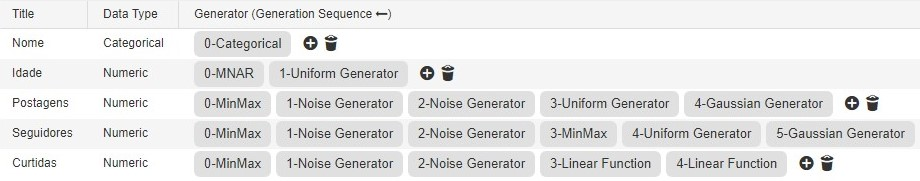
\includegraphics[width=\linewidth]{./figures/Resultados/RSmodelo.jpg}
			\label{fig:RSmodelo}
			\footnotesize Fonte: O autor do trabalho.
		\end{figure}

		Mais duas dimensões são disponibilizadas e também complexas.
		Entre elas estão a dimensão Seguidores que possui uma forte discrepância, para simular grandes famosos, mas são muito raros.
		E ainda a dimensão Curtidas, que possui correlação de Seguidores - cerca de 60\% das curtidas são de seguidores - e postagens - quanto mais postagens, mais curtidas acumuladas.
		Além da correlação, possui a discrepância fraca e muito forte, para simular boas postagens e postagens virais.
		\par

		% Por conseguinte a terceira base, vista na figura \ref{fig:BEmodelo}, diz respeito a um Boletim Escolar que possui
		%  um nome de aluno (categoria genérica);
		%  dimensão de Frequência, a qual possui uma média em 75\%, podendo variar para cima ou para baixo e com discrepâncias como frequência máxima e sem frequência;
		%  Matérias que é distribuída uniformemente;
		%  E CRG (Coeficiente de Rendimento Geral) que possui uma origem de valor com média 5, 
		%   possui correlação inversamente proporcional com matérias, 
		%   diretamente proporcional com frequência,
		%   E uma pequena porcentagem de alunos que tiram nota alta sem essa correlação são exemplos de dados discrepantes.
		% \par
		% \begin{figure}[h!]
		% 	\centering
		% 	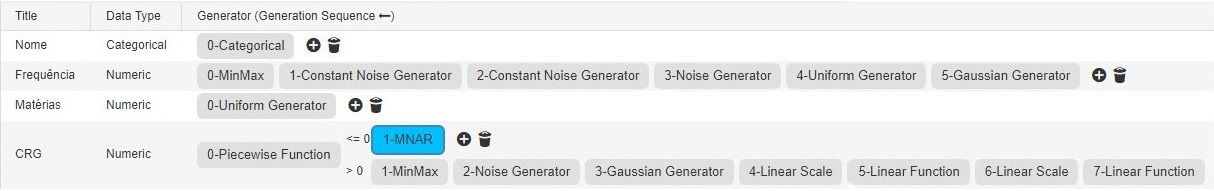
\includegraphics[width=\linewidth]{./figures/Resultados/BEmodelo.jpg}
		% 	\caption{Base sintética de avaliação de Boletim Escolar.}
		% 	\label{fig:BEmodelo}
		% \end{figure}

		% A base de Atletismo (ver figura \ref{fig:AtletaModelo}) foi criada para simular um cenário de dados em relação ao tempo.
		% Para isso tem um atleta, um valor categórico qualquer;
		% Uma modalidade que é o quanto um atleta corre em uma competição (100 a 400 metros);
		% Marcação é o valor temporal do instante em que foi marcado;
		% Distância é, dado o instante, o quanto o atleta percorreu, o qual é baseado na sua modalidade;
		% E a última dimensão diz respeito à frequência cardíaca no instante.
		% A base de Atletismo foi levemente alterada para introdução do gerador MAR em vez de uma função Linear, como visto na figura \ref{fig:AtletaModeloMAR}
		\par
		% \begin{figure}[h!]
		% 	\centering
		% 	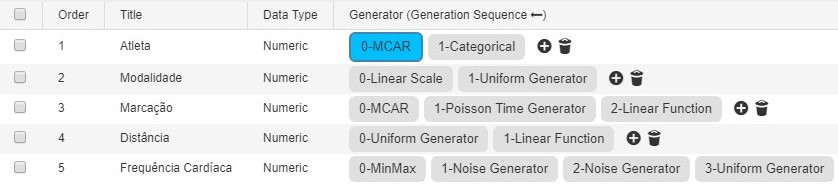
\includegraphics[width=\linewidth]{./figures/Resultados/AtletaModelo.jpg}
		% 	\caption{Base sintética de avaliação de atletas.}
		% 	\label{fig:AtletaModelo}
		% \end{figure}
		% \begin{figure}[h!]
		% 	\centering
		% 	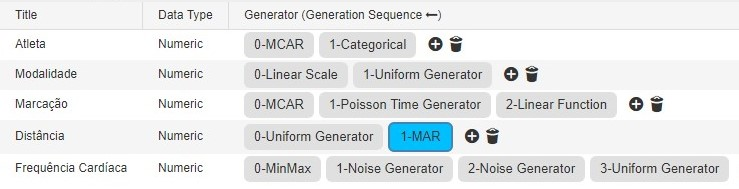
\includegraphics[width=\linewidth]{./figures/Resultados/AtletismoModeloMAR.jpg}
		% 	\caption{Base sintética de avaliação de atletas com MAR.}
		% 	\label{fig:AtletaModeloMAR}
		% \end{figure}

		
		A terceira base como pode ser visto na figura \ref{fig:CMModelo} mostra um esquema de convênios médicos.
		Primeiramente há o profissional e sua especialidade - ambos dados categóricos uniformes;
		Quanto ao Plano de saúde - é referente aos que atende - e esta dimensão possui um peso, devido à popularidade e/ou acessibilidade dos planos;
		E o Preço da Consulta varia de acordo com o plano de saúde.
		Para essa variação foram escolhidos vários geradores da categoria aleatória com parâmetros diferentes, com o intuito de gerar dados discrepantes sem utilizar o gerador \emph{Noise Generator}.
		\par
		\begin{figure}[h!]
			\centering
			\caption{Base sintética de avaliação de Convênios Médicos.}
			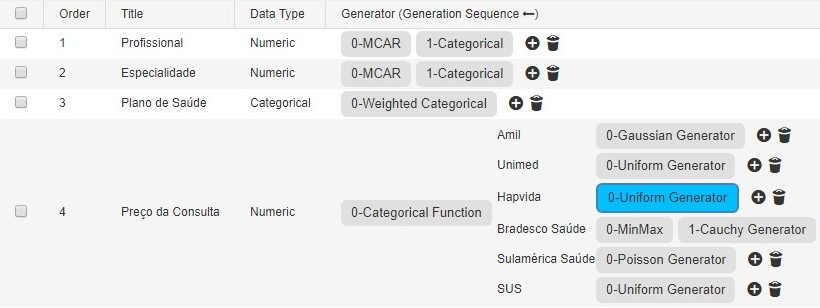
\includegraphics[width=\linewidth]{./figures/Resultados/CMModelo.jpg}
			\label{fig:CMModelo}
			\footnotesize Fonte: O autor do trabalho.
		\end{figure}

		A base que simula uma estrutura de conta bancária (ver figura \ref{fig:BancoModelo}) foi feita com a intenção de mostrar dados hierárquicos.
		A identificação de uma conta bancária é composta três campos sendo eles: 
		 um banco composto por 3 dígitos,
		 uma agência de 4 dígitos e 
		 uma conta composta por 8 dígitos.
		Foram acrescentados umas opções de dados faltantes do tipo MCAR e MNAR.

		\begin{figure}[h!]
			\centering
			\caption{Base sintética de avaliação de Estrutura de Conta Bancária.}
			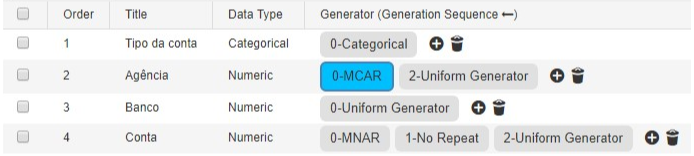
\includegraphics[width=\linewidth]{./figures/Resultados/BancoModelo.png}
			\label{fig:BancoModelo}
			\footnotesize Fonte: O autor do trabalho.
		\end{figure}

		Há também uma base genérica como vista na figura \ref{fig:BaseGenerica} com o intuito de mostrar os dados faltantes de uma forma mais simples.
		A primeira dimensão é chamada de dimensão observada, que é a dimensão utilizada para predizer dados faltantes no mecanismo MAR.
		A segunda dimensão possui dados faltantes a partir do mecanismo MAR.
		A terceira dimensão possui dados faltantes a partir do mecanismo MCAR. 
		E a quarta dimensão possui dados faltantes a partir do mecanismo MNAR.

		\begin{figure}[h!]
			\centering
			\caption{Base sintética genérica para geração de dados faltantes numéricos.}
			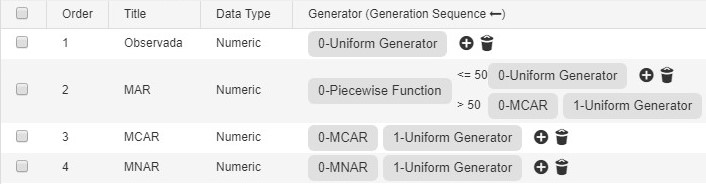
\includegraphics[width=\linewidth]{./figures/Resultados/BaseGenericaModelo.jpg}
			\label{fig:BaseGenerica}
			\footnotesize Fonte: O autor do trabalho.
		\end{figure}

		% Em suma, na tabela \ref{table:resumo caracteristica dimensao bases de validacao} é possível encontrar um pequeno resumo das características peculiares das dimensões de cada base sintética gerada.
		% O objetivo dessa tabela é facilitar a visualização e comparação do pretendido e dos resultados obtidos que serão mostrados na sessão de validação.
		% \begin{table}[htb]
		% 	\center
		% 	\caption{Tabela de Resumo das características das dimensões das bases de validação.
		% 	}
		% 	\label{table:resumo caracteristica dimensao bases de validacao}
		% 	\begin{tabular}{l|l|l|l}
		% 		Base            & Dimensão          & Característica(s)                                         & Grau Esperado\\
		% 		\hline
		% 		Carros          & Categoria         & U\footnotemark[1]                                         & Normal\\
		% 		Carros          & Ano               & U\footnotemark[1]                                         & Normal\\
		% 		Carros          & Marca             & U\footnotemark[1]                                         & Normal\\
		% 		Carros          & Preço             & Di\footnotemark[2] e C\footnotemark[3]                    & Leve\\
		% 		Carros          & Nota dos Críticos & U\footnotemark[1] e F\footnotemark[4]                     & Leve\\
		% 		Carros          & Nota do público   & De\footnotemark[5], F\footnotemark[4] e C\footnotemark[3] & Mediano\\
		% 		Redes Sociais   & Nome              & U\footnotemark[1]                                         & Normal\\
		% 		Redes Sociais   & Idade             & U\footnotemark[1] e F\footnotemark[4]                     & Mediano\\
		% 		Redes Sociais   & Postagens         & G\footnotemark[6], Di\footnotemark[2]                     & Alto\\
		% 		Redes Sociais   & Seguidores        & G\footnotemark[6], Di\footnotemark[2]                     & Extremo\\
		% 		Redes Sociais   & Curtidas          & Di\footnotemark[2] e C\footnotemark[3]                    & Extremo\\
		% 		Boletim Escolar & Nome              & U\footnotemark[1]                                         & Normal\\
		% 		Boletim Escolar & Frequência        & G\footnotemark[6], Di\footnotemark[2]                     & Leve\\
		% 		Boletim Escolar & Matérias          & U\footnotemark[1]                                         & Normal\\
		% 		Boletim Escolar & CRG               & De\footnotemark[5], F\footnotemark[4] e C\footnotemark[3] & Mediano\\
		% 	\end{tabular}
		% \end{table}

		% \footnotetext[1]{Uniforme}
		% \footnotetext[2]{Discrepante}
		% \footnotetext[3]{Correlacional}
		% \footnotetext[4]{Faltante}
		% \footnotetext[5]{Decisional}
		% \footnotetext[6]{Gaussiano}
		
	\section{Apresentação das Visualizações}
	Uma vez que o modelo está pronto é preciso visualizar os dados e analisar os seus resultados.
	O Blocks possui um sistema de visualização integrado (\emph{VisApplication}) e suas visualizações são utilizadas como exemplos.
	Entretanto, outras aplicações foram utilizadas para visualização de dados como o RAWGraphs \cite{rawGraphs} e o Excel \cite{excel}.
	\par

	Para a base de Carros foram utilizadas duas técnicas de visualizações de dados, Coordenadas Paralelas e Scatterplot.
	Na figura \ref{fig:PCCarros}, a qual possui três gráficos de coordenadas paralelas agrupadas.
	Os gráficos se diferenciam na origem da coloração dos dados.
	O gráfico mais em cima tem como origem a dimensão Preço, o do meio tem Nota dos críticos e o mais embaixo tem a Nota do público.
	\par
	Nessa visualização é possível perceber a grande quantidade de carros baratos, por conta da predominância de linhas azuis (marcação alaranjada) no primeiro gráfico e há uma forte correlação com o ano (marcação cinza) e possuem, em geral, uma alta nota dos críticos e do público (Marcação rosa).
	Pode-se perceber um vácuo nas notas 1 e 2 (marcação verde) na dimensão das Notas dos críticos, o que é resultado do gerador MNAR.
	Também é observável a correlação (marcação rosa) entre as notas do críticos e nota do público.
	\par
	Na figura \ref{fig:ScatterPlotC} mais detalhes podem ser percebidos por conta da dispersão.
	Primeiramente, os valores abaixo de 0 (marcação verde) são os dados faltantes.
	Esse padrão é adotado não só nesse modelo de dados.
	\par
	Ainda na figura \ref{fig:ScatterPlotC}, encontra-se a correlação entre Nota do público e dos Críticos (Marcação vermelha).
	No preço, há um vácuo na faixa de 80.000 (marcação cinza), apesar de não ter sido intencional, caracteriza-se um MNAR, pois a resposta não está na base de dados.
	Sobre a correlação, é possível perceber com mais clareza a correlação diretamente proporcional entre nota dos críticos e do público (marcação vermelha), e uma leve correlação inversamente proporcional entre preço e nota do público (marcação alaranjada) e também entre preço e ano (marcação em roxo).
	\par

	\begin{figure}[h!]
		\centering
		\caption{Visualização Coordenadas Paralelas da base de carros.}
		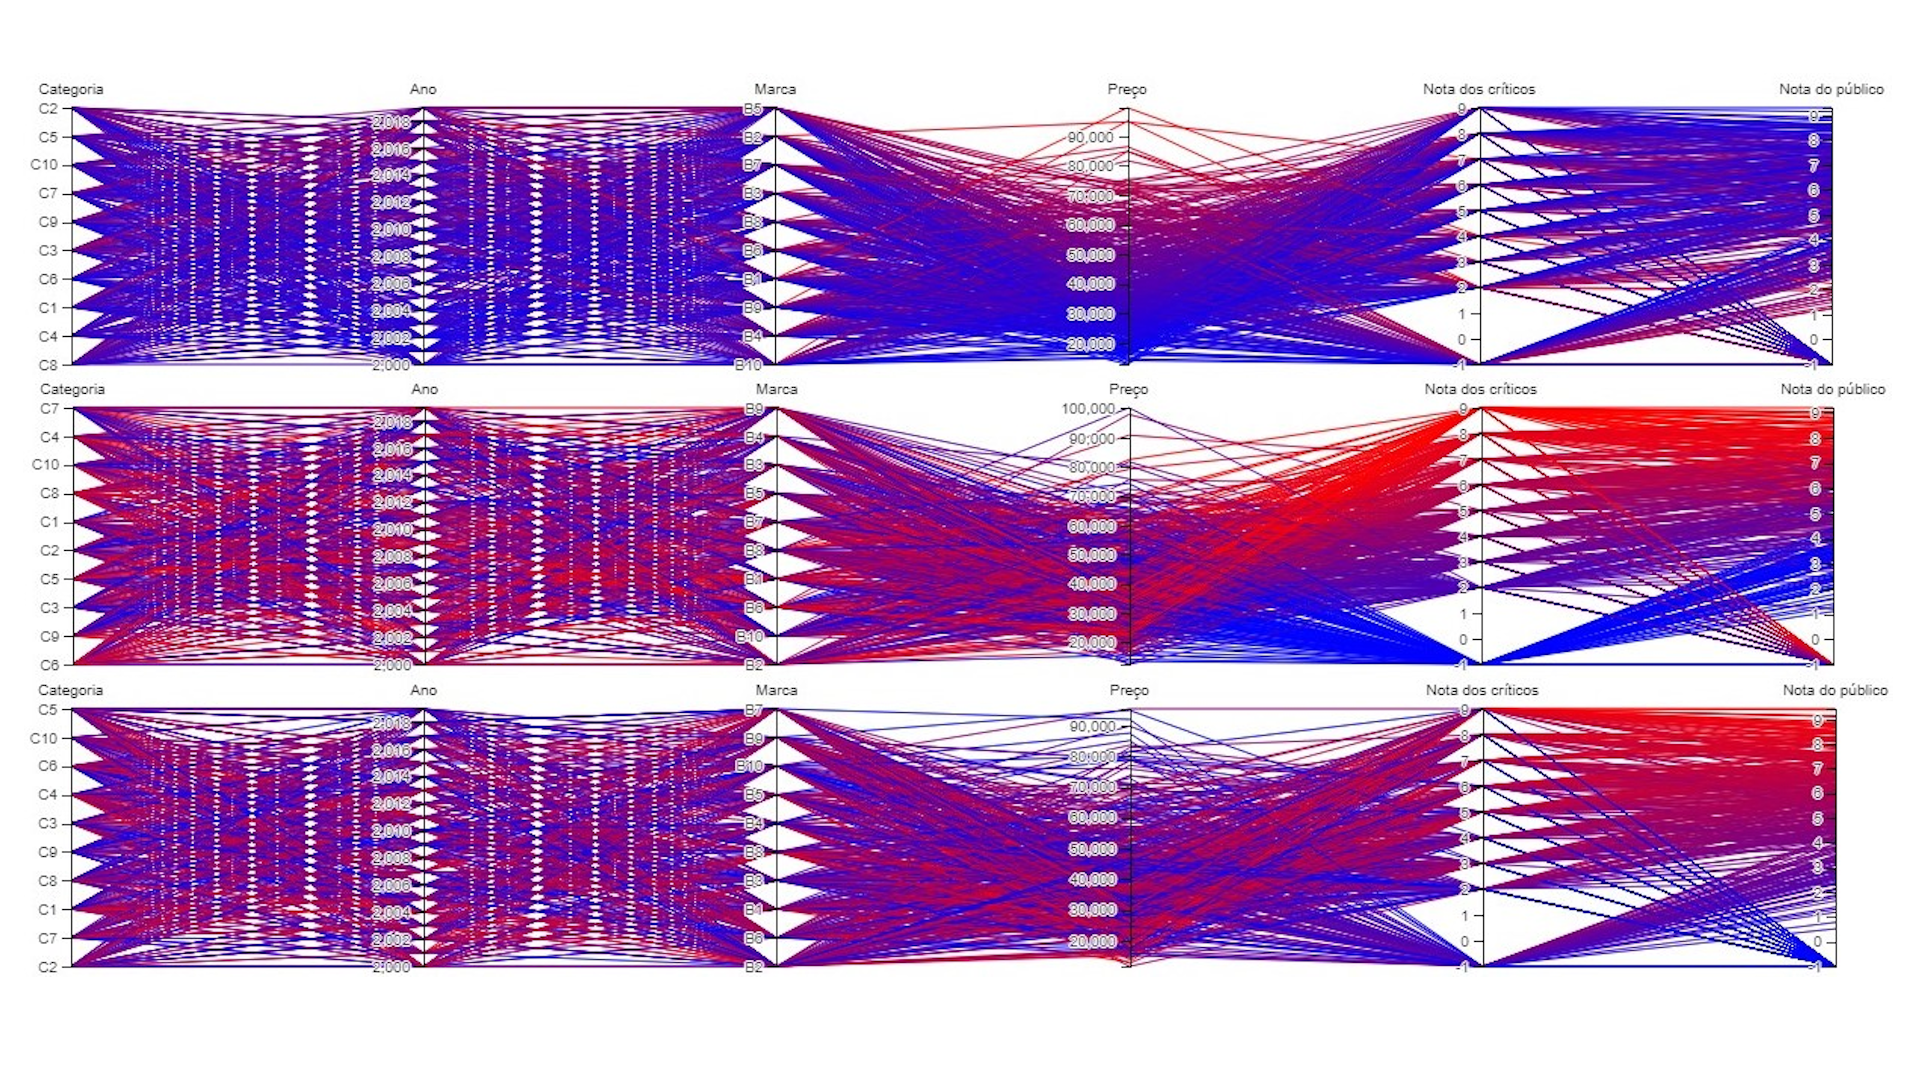
\includegraphics[width=\linewidth]{./figures/Resultados/PCCarros.png}
		\label{fig:PCCarros}
		\footnotesize Fonte: O autor do trabalho.
	\end{figure}

	\begin{figure}[h!]
		\centering
		\caption{Visualização Scatterplot da base de carros.}
		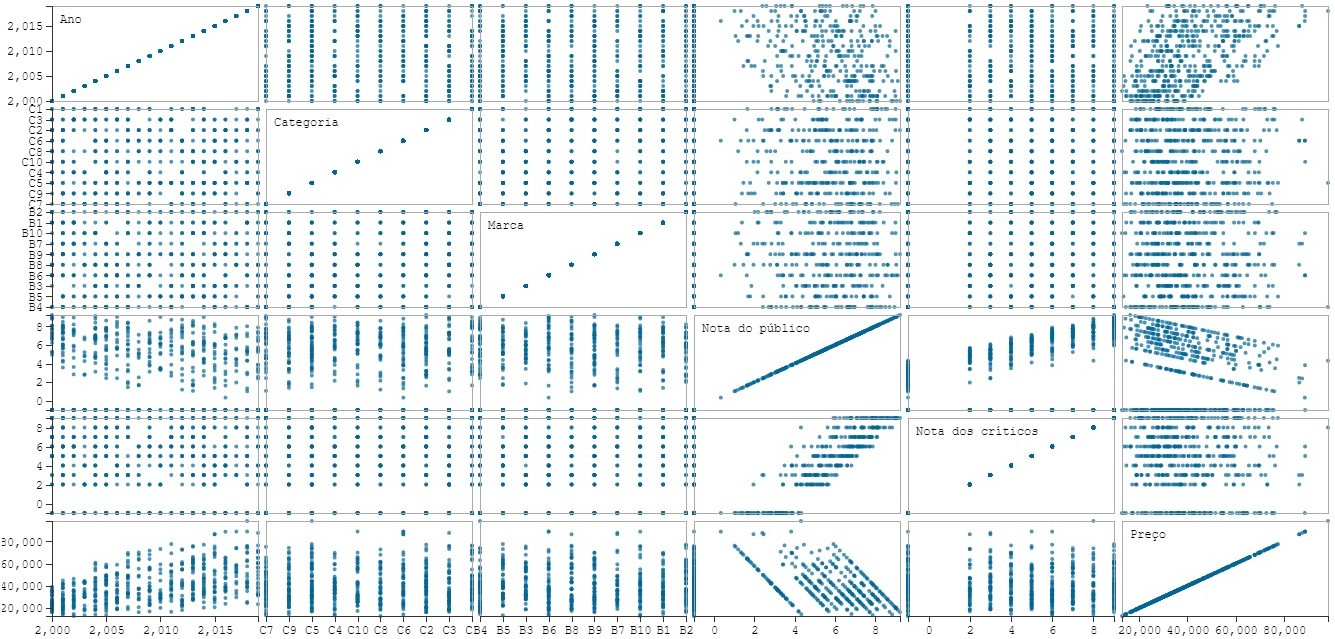
\includegraphics[width=\linewidth]{./figures/Resultados/ScatterPlotC.jpg}
		\label{fig:ScatterPlotC}
		\footnotesize Fonte: O autor do trabalho.
	\end{figure}

	A figura \ref{fig:PCRS} apresenta as principais características do modelo de dados sobre Redes Sociais.
	Na dimensão Idade é possível encontrar dados faltantes a partir dos 40 anos (marcação alaranjada), logo, caracteriza-se um MNAR, pois não está na base de dados a explicação.
	E os dados discrepantes nas dimensões de seguidores, curtidas e postagens.
	É possível identificar exemplos de dados discrepantes ruidosos (marcação verde) e anômalos (marcação vermelha)
	O padrão encontrado é que as pessoas possuam uma faixa de duas mil postagens, menos de cinco milhões de seguidores e menos de quinhetas mil curtidas no total.
	E por conta dos dados discrepantes, a própria escala é prejudicada.
	\par

	No histograma (ver figura \ref{fig:HistogramaRS}) é possível visualizar a questão da escala dos dados.
	A frequência dos dados numa mesma coluna e muito pouco ou nada nas outras ratifica o problema do alto grau de discrepância da base.
	Este problema pode ser visto nas dimensões de Curtida, Postagens e Seguidores (marcação alaranjada).
	Em Idade, pode ser visto uma alta frequência de dados faltantes, mas uma frequência melhor distribuída (marcação em verde).
	\par

	\begin{figure}[h!]
		\centering
		\caption{Visualização Coordenadas Paralelas da base de Redes Sociais.}
		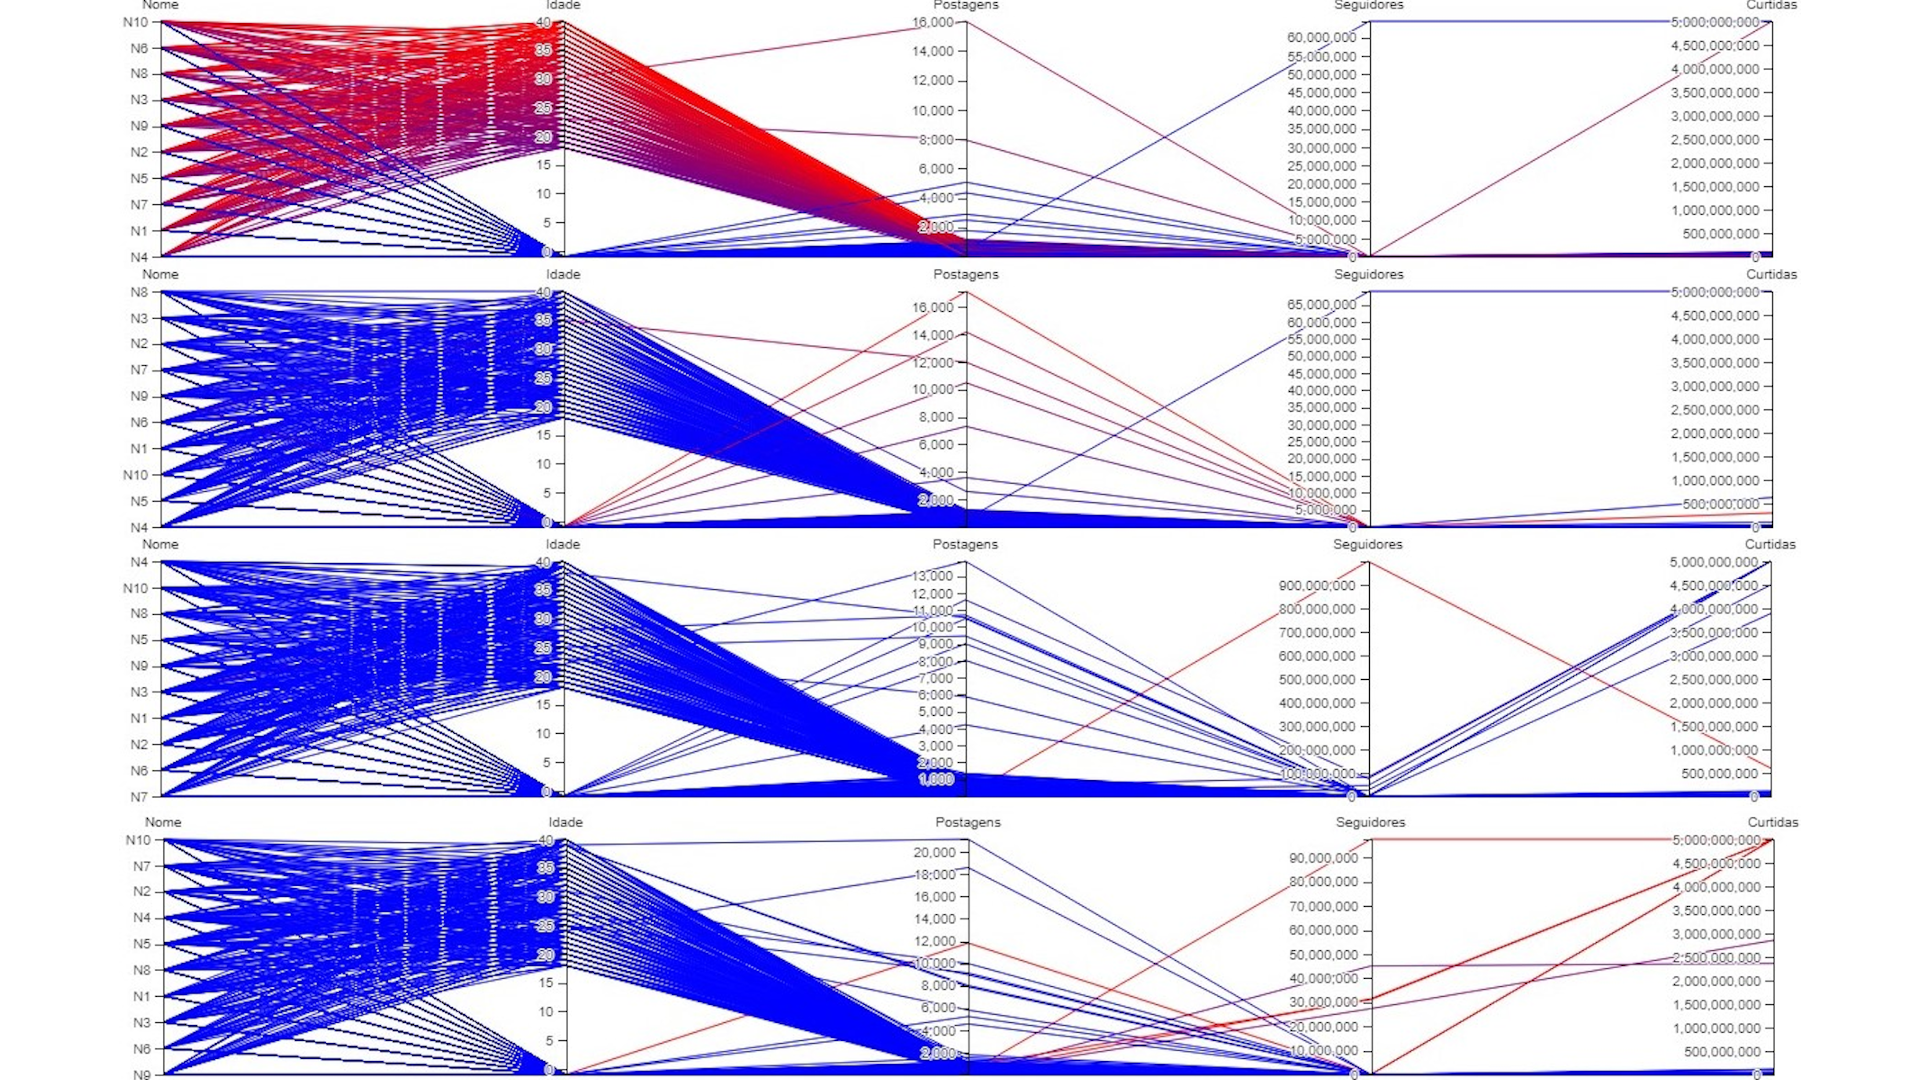
\includegraphics[width=\linewidth]{./figures/Resultados/PCRS.png}
		\label{fig:PCRS}
		\footnotesize Fonte: O autor do trabalho.
	\end{figure}

	\begin{figure}[h!]
		\centering
		\caption{Visualização Histograma da base de Redes Sociais. A unidade de Curtida é bilhões; Seguidores está em milhões e Postagens está em milhares.}
		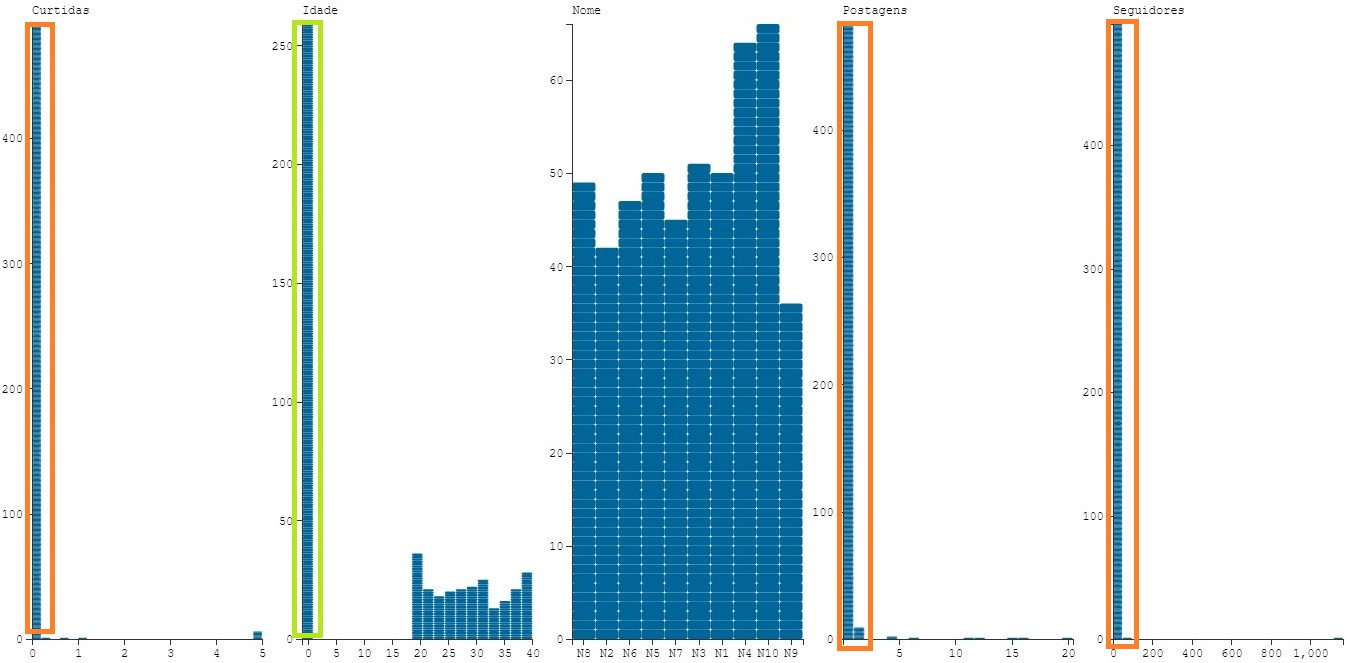
\includegraphics[width=\linewidth]{./figures/Resultados/HistogramaRS.jpg}
		\label{fig:HistogramaRS}
		\footnotesize Fonte: O autor do trabalho.
	\end{figure}

	% A figura tal mostra a visualização coordenadas paralelas referente ao modelo Boletim Escolar.
	% Sem muito esforço, é possível perceber a correlação entre CRG e frequência.
	% Há um vácuo não intencional na frequência e pode ser caracterizado um MCAR.


	% \begin{figure}[h!]
	% 	\centering
	% 	\includegraphics[width=\linewidth]{./figures/Resultados/PCBE.png}
	% 	\caption{Visualização Coordenadas Paralelas da base de Boletim Escolar.}
	% 	\label{fig:PCBE}
	% \end{figure}

	% \begin{figure}[h!]
	% 	\centering
	% 	\includegraphics[width=\linewidth]{./figures/Resultados/ScatterPlotBE.jpg}
	% 	\caption{Visualização Scatterplot da base de Boletim Escolar.}
	% 	\label{fig:ScatterPlotBE}
	% \end{figure}

	As visualizações das bases anteriores foram geradas pelo \emph{VisApplication} e o \emph{Preview} do Blocks.
	As visualizações do modelo de base genérica foram geradas no Excel, utilizando os gráficos de linha, pontos e colunas agrupadas.
	\par
	% Na figura \ref{fig:Atletismo-Marcacao-Distancia} mostra a relação marcação-distância.
	% Percebe-se que há muitos dados nas extremidades e muitos dados abaixo da faixa de 150 de distância.
	% Contudo, ao se comparar com a marcação-distância (ver figura \ref{fig:Atletismo-Frequencia-Distancia}) não há uma correlação - por exemplo, uma alta distância percorrida em menos tempo tente a aumentar a frequência cardíaca.
	% Isso acontece porque não há um gerador para correlacionar dados temporais e dados numéricos na aplicação Blocks.
	% Por isso, são dados discrepantes ainda que não intencionais.
	% E para melhorar a visualização dos faltantes foi utilizado o Matrix Plot (ver figura \ref{fig:Atletismo-Matrix-Plot}), contudo, foi diminuida para 50 instâncias a quantidade de dados, para não haver sobreposição dos dados.
	\par

	% \begin{figure}[h!]
	% 	\centering
	% 	\includegraphics[width=\linewidth]{./figures/Resultados/Atletismo-Marcacao-Distancia.png}
	% 	\caption{Visualização Gráfico de linha da base de atletas.}
	% 	\label{fig:Atletismo-Marcacao-Distancia}
	% \end{figure}

	% \begin{figure}[h!]
	% 	\centering
	% 	\includegraphics[width=\linewidth]{./figures/Resultados/Atletismo-Frequencia-Distancia.png}
	% 	\caption{Visualização de Gráfico de Ponto da base de atletas.}
	% 	\label{fig:Atletismo-Frequencia-Distancia}
	% \end{figure}

	% \begin{figure}[h!]
	% 	\centering
	% 	\includegraphics[width=\linewidth]{./figures/Resultados/AtletismoMatrixPlot.jpg}
	% 	\caption{Visualização Matrix Plot da base de atletas.}
	% 	\label{fig:Atletismo-Matrix-Plot}
	% \end{figure}

	O modelo de dados sobre estruturas de conta bancária possui uma arquitetura hierárquica e pode ser vista por meio do uso de um Dendrograma (ver figura \ref{fig:BancoDendrograma}).
	A priori, para esta visualização foi necessário reduzir a 10\% - 50 instâncias - o volume de dados, para que as propriedades hierárquicas possam ser percebidas.
	Na visualização é possível identificar dados faltantes do tipo MCAR, visto que, foram perdidas de forma aleatória, mas não foi imaginada uma forma de gerar dados discrepantes.
	Também percebe-se que os valores faltantes foram repetidos para que não fosse afetada a propriedade dos dados hierárquicos.
	% E também na figura \ref{fig:BancoMatrixPlot} é possível encontrar os dados faltantes através do gráfico de matriz.
	\par
	\begin{figure}[h!]
		\centering
		\caption{Visualização Dendrograma da base sobre estrutura de conta bancária.}
		\includegraphics[width=\linewidth]{./figures/Resultados/BancoDendrograma.png}
		\label{fig:BancoDendrograma}
		\footnotesize Fonte: O autor do trabalho.
	\end{figure}

	% \begin{figure}[h!]
	% 	\centering
	% 	\includegraphics[width=\linewidth]{./figures/Resultados/BancoMatrixPlot.jpg}
	% 	\caption{Visualização Matrix Plot da base sobre os dados faltantes de conta bancária.}
	% 	\label{fig:BancoMatrixPlot}
	% \end{figure}

	Na figura \ref{fig:BCCM} é possível ver um gráfico de barras subagrupado por especialidades médicas.
	Neste gráfico pode-se comparar os valores de cada especialidade por plano de saúde.
	Primeiramente, o SYS1 possui uma discrepância anômala, pois os dados são próximos de 0 - fora adicionados valores ínfimos para que não seja confundido com um dado faltante.
	Os dados faltantes são representados por uma barra sem tamanho.
	É possível identificar que há discrepância nos dados, mas não foi utilizado um gerador específico, apenas uma função categórica e diferentes geradores de dados, os quais foram escolhidos com o intuito de gerar um comportamento discrepante.

	\begin{figure}[h!]
		\centering
		\caption{Visualização Gráfico de Colunas da base Convênios Médicos. Eixo X: Planos de Saúde, Eixo Y: Especialidades, Barra: Preço por Consulta}
		\includegraphics[width=\linewidth]{./figures/Resultados/BCCM.png}
		\label{fig:BCCM}
		\footnotesize Fonte: O autor do trabalho.
	\end{figure}

	Também foi gerada uma base genérica para visualização dos mecanismo de dados faltantes e essas podem ser vistas na figura \ref{fig:MVMatrixPlot}.
	As duas dimensões à esquerda foram ordenadas juntas, as outras foram dissociadas para que fossem mantidas as propriedades dos dados faltantes.
	Na figura percebe-se que os valores da dimensão MAR podem ser previstos a partir da dimensão Observada.
	A dimensão MCAR possui dados faltantes espalhados, ilustrando um comportamento completamentamente aleatório.
	E a coluna MNAR possui somente seus valores mais baixos como dados faltantes, o que pode te0r uma explicação fora da base de dados.
	
	\begin{figure}[h!]
		\centering
		\caption{Visualização Gráfico de Colunas da base genérica para visualização de dados faltantes.}
		\includegraphics[width=\linewidth]{./figures/Resultados/MVMatrixPlot.png}
		\label{fig:MVMatrixPlot}
		\footnotesize Fonte: O autor do trabalho.
	\end{figure}
	

% ---
% Conclusão
% ---
\chapter{Considerações Finais e Trabalhos Futuros}
% ---

O desenvolvimento do presente trabalho proporcionou a análise da geração de dados sintéticos discrepantes e faltantes na aplicação Blocks.
O sistema é \emph{Open Source} e permite a geração e visualização de dados sintéticos e implementação de novos recursos ao sistema.
\par
Os dados sintéticos são importantes para mais variadas aplicações, por conta da seu desvínculo com a confidencialidade dos dados.
O fato de geração basear-se em modelos permite que o compartilhamento dos dados seja mais leve, mas exigindo do processamento em contrapeso.
A utilização (modelagem, geração ou visualização) gratuita de dados sintéticos permite que a pesquisa e teste de aplicações seja fomentado e democratizado, pois é acessível para todos.
\par
O Blocks é um sistema competente no que diz respeito à modelagem e geração de dados sintéticos.
Sua geração de dados é baseada em modelos, os quais por sua vez possuem blocos de geradores que podem ser encadeados.
Esse encadeamento permite que o comportamento dos dados sejam mais complexos, o que distancia de dados mais previsíveis e comuns.
Além do encadeamento, o sistema possui uma vasta gama de geradores, desde sequenciais, aleatórios, funcionais, acessórios e geométricos, os quais permitem que o usuário crie variados cenários e níveis de abstração.
\par
O Blocks também permite que esses dados sejam distribuídos via \emph{Web Service};
 salvos em arquivos - CSV, JSON, TSV;
 O sistema permite visualizar os modelos de dados de forma rápida e prática ou de forma mais detalhada e diversa com a integração com o \emph{VisApplication}.
\par
Nos resultados apresentados na seção Validação Visual, os dados faltantes do mecanismo MCAR apresentaram a característica aleatória dada uma taxa de ausência. 
No MAR, os dados também foram faltantes, mas foi possível enxergar correlação entre as dimensões que possui a ausência e a dimensão observada. 
O gerador do mecanismo MNAR permite que os dados faltem dada uma lógica - para simular um motivo fora da base de dados.
Portanto, de forma geral, a aplicação permitiu que as características - dados faltantes e discrepantes - fossem percebidas no conjunto de dados de forma satisfatória, como vista na seção de Validação Visual, pois além da discrepância e falta de dados, também foi possível fazer correlações.
\par
Os mecanismos de dados faltantes são utilizados para entender porquê aquele dado está faltando.
São três mecanismos: \emph{Missing Completely At Random} (MCAR), \emph{Missing At Random} (MAR) e \emph{Missing Not At Random} (MNAR).
O mecanismo MCAR é utilizado quando o motivo do dado está faltando não pode ser previsto pela base de dados nem por fatores externos, por isso é dito como completamente aleatório.
O MAR é utilizado quando o dado está faltando por um motivo qualquer, mas seu valor pode ser previsto por meio de alguma dimensão dentro da base dados.
Quanto ao MNAR, este mecanismo é utilizado quando o dado está faltando por algum fator externo à base de dados.
\par
Quanto aos dados discrepantes, os quais podem ser subclassificados em ruidosos e anômalos, tem como principal característica um limiar entre eles.
Isso porque dados discrepantes podem existir por um valor muito distante dos outros, ou por um caractere alfabético em uma dimensão numérica, ou uma palavra embaralhada, entre outros.
Ou seja, o que determina um dado ser ruidoso ou anômalo é o seu impacto na análise dos dados, como a referência distorcida de escala dos dados em gráficos, média dos valores da base de dados muito mais alta ou baixa do que sem os dados discrepantes etc.
\par
Para propor trabalhos futuros para os problemas vistos, é interessante que o Blocks possua mais geradores categóricos, como gerar a partir de uma expressão regular, a partir de um arquivo, geração de anagramas datas as letras ou uma categoria, permitir embaralhar categorias etc.
Um gerador temporal sazonal, que possui a estrutura de encadeamento similar ao \emph{TimeLaps Function}.
Alguns acessórios também são interessantes como formatar números de diferentes geradores - como ter números discretos ou com casas decimais fixas.
Também testes de exaustão com o objetivo de otimizar o número de instâncias de cada bloco para geração de dados. 
\par

% ----------------------------------------------------------
% ELEMENTOS PÓS-TEXTUAIS
% ----------------------------------------------------------
\postextual
% ----------------------------------------------------------

% ----------------------------------------------------------
% Referências bibliográficas
% ----------------------------------------------------------
\bibliography{abntex2-modelo-references}


% \appendix
% \addcontentsline{page}{chapter}{APÊNDICES}

\part*{Apêndices} % se quiser uma página antes dos apêndices
\chapter*{Apêndice A -- Atalhos do Teclado da aplicação Blocks}
\addcontentsline{toc}{chapter}{Apêndice A -- Atalhos do Teclado da aplicação Blocks}
			Modelar um conjunto de dados pode ser exaustivo, portanto, alguns atalhos podem facilitar na prevenção e correção de erros, eficiência e economia de esforço e afins.
			Visando dar praticidade ao usuário, o Block Data Generator possui atalhos de teclados que podem ser vistos na tabela \ref{table: comandos do teclado}.
				\begin{table}[h]
					\centering
					\caption{Tabela de atalhos do teclado do Blocks.}
					\vspace{0.5cm}
					\label{table: comandos do teclado}
					\begin{tabular}{r|lll}
					
						Nome                 & Comando          & Descrição                           \\ % Note a separação de col. e a quebra de linhas
						\hline                                  % para uma linha horizontal
						\emph{New Model}     & Ctrl/Cmd+M       & Cria novo modelo.                   \\
						\emph{Delete Model}  & Ctrl/Cmd+W       & Deleta modelo atual.                \\
						\emph{New Dimension} & Ctrl/Cmd+D       & Cria nova dimensão.                 \\
						\emph{Open Model}    & Ctrl/Cmd+O       & Insere um modelo no sistema.        \\
						\emph{Save Model}    & Ctrl/Cmd+S       & Salva as alterações do modelo atual.\\
						\emph{Undo}          & Ctrl/Cmd+Z       & Desfaz uma alteração.               \\
						\emph{Redo}          & Ctrl/Cmd+Shift+Z & Refaz uma alteração.                \\
			
					\end{tabular}
					\bigskip
					\\
					\footnotesize Fonte: O autor do trabalho.
				\end{table}
			\par
			
			Além de acesso pelo teclado, os atalhos podem ser acessados pela barra superior da tela inicial (ver figura \ref{fig:telaPrincipal}) (22).
			É válido ressaltar sobre a questão de edição da modelagem, que o Blocks salva as mudanças no automaticamente em arquivo separado, o qual pode ser recuperado se não forem salvas/descartadas adequadamente.

\end{document}
 